%\documentclass[aps,prb,onecolumn,nofootinbib]{revtex4}  
\documentclass[12pt,a4paper]{article}
\usepackage[margin=1in]{geometry}  % set the margins to 1in on all sides
%\usepackage{jheppub}
\usepackage{amsmath,amsfonts,amssymb,latexsym,dsfont}
\usepackage{hhline}
\usepackage{graphicx}
%\usepackage[arrow,matrix]{xy}
\usepackage[all]{xy}
\usepackage{tikz}
\usepackage{tikz-cd}
\definecolor{hanpurple}{rgb}{0.32, 0.09, 0.98}

\usepackage{tabu}

\usepackage[numbers]{natbib}
\usepackage[colorlinks]{hyperref}
\hypersetup{linkcolor={hanpurple}}




\usetikzlibrary{positioning,arrows}
\usetikzlibrary{decorations.pathmorphing}
\usetikzlibrary{decorations.markings}

\usetikzlibrary{decorations.pathreplacing,calc}

\newcommand{\tikzmark}[2][-3pt]{\tikz[remember picture, overlay, baseline=-0.5ex]\node[#1](#2){};}

\tikzset{brace/.style={decorate, decoration={brace}},
 brace mirrored/.style={decorate, decoration={brace,mirror}},
}

\newcounter{brace}
\setcounter{brace}{0}
\newcommand{\drawbrace}[3][brace]{%
 \refstepcounter{brace}
 \tikz[remember picture, overlay]\draw[#1] (#2.center)--(#3.center)node[pos=0.5, name=brace-\thebrace]{};
}

\newcounter{arrow}
\setcounter{arrow}{0}
\newcommand{\drawcurvedarrow}[3][]{%
 \refstepcounter{arrow}
 \tikz[remember picture, overlay]\draw (#2.center)edge[#1]node[coordinate,pos=0.5, name=arrow-\thearrow]{}(#3.center);
}

% #1 options, #2 position, #3 text 
\newcommand{\annote}[3][]{%
 \tikz[remember picture, overlay]\node[#1] at (#2) {#3};
}

\newcommand{\tp}{\otimes}
\newcommand{\tpc}{\tilde{\otimes}}
\newcommand{\ra}{\rightarrow}
\newcommand{\unit}{\mathds{1}}
\newcommand{\zz}{\mathbb{Z}}
\newcommand{\mce}{\mathcal{E}}
\newcommand{\cc}{\mathbb{C}}
\newcommand{\rr}{\mathbb{R}}
\newcommand{\mcr}{\mathcal{R}}
\newcommand{\mcz}{\mathcal{Z}}
\newcommand{\mca}{\mathcal{A}}
\newcommand{\mcd}{\mathcal{D}}
\newcommand{\mcg}{\mathcal{G}}
\newcommand{\mct}{\mathcal{T}}
\newcommand{\mcs}{\mathcal{S}}
\newcommand{\ul}{\underline}
\newcommand{\Mod}{\text{Mod}}
\newcommand{\Aut}{\text{Aut}}
\newcommand{\ulmcc}{\underline{\mathcal{C}}}
\newcommand{\zt}{\mathbb{Z}_2}
\newcommand{\oeo}{\text{others = 1}}
\newcommand\be            {\begin{equation}}
\newcommand\ee            {\end{equation}}
\newcommand\ba            {\begin{aligned}}
\newcommand\ea            {\end{aligned}}
\newcommand{\mcf}{\mathcal{F}}
\newcommand{\spinz}{\text{\sffamily{Z}}}
\newcommand{\spinx}{\text{\sffamily{X}}}
\newcommand{\mcl}{\mathcal{L}}
\newcommand{\mcc}{\mathcal{C}}
\newcommand{\mco}{\mathcal{O}}
\newcommand{\mcm}{\mathcal{M}}
\newcommand{\zc}{\mathcal{Z}(\mathcal{C})}
\newcommand{\id}{\text{id}}
\newcommand{\Hom}{\text{Hom}}
\newcommand{\End}{\text{End}}
\newcommand{\Tor}{\text{Tor}}
\newcommand{\Ext}{\text{Ext}}
\newcommand{\p}{\partial}
\newcommand{\wt}{\widetilde}
\usepackage{verbatim}
\newcommand{\cl}{\mathbb{C}\ell}
\newcommand{\vect}{\text{Vec}}
\newcommand{\svect}{\text{sVec}}
\newcommand{\spin}{\text{Spin}}
\newcommand{\pin}{\text{Pin}}
\newcommand{\fube}{\textbf{Tube}}
\newcommand{\tube}{\textbf{Tube}}
\newcommand{\fld}{\mathcal{F}} %fld was for field config

\newcommand{\bra}[1]{\ensuremath{\left\langle#1\right|}}
\newcommand{\ket}[1]{\ensuremath{\left|#1\right\rangle}}

\definecolor{ao(english)}{rgb}{0.0, 0.5, 0.0}
\definecolor{americanrose}{rgb}{1.0, 0.01, 0.24}
\definecolor{amber(sae/ece)}{rgb}{1.0, 0.49, 0.0}

\newcommand{\dave}[1]{{\color{ao(english)}\footnotesize{(DA) #1}}}
\newcommand{\remove}[1]{{\color{amber(sae/ece)}\footnotesize{(RM?) #1}}}

%a purple that looks different from red. EL: nice! I like the name
\definecolor{amethyst}{rgb}{0.6, 0.4, 0.8}
\newcommand{\ethan}[1]{{\color{amethyst}\footnotesize{(EL) #1}}}

\definecolor{kwcolor}{rgb}{0.2, 0.5, 0.85}
\newcommand{\kw}[1]{{\color{kwcolor}\footnotesize{(KW) #1}}}
\newcommand{\kwsep}{\bigskip\hrule\medskip\hrule\medskip\hrule\bigskip}

\newcommand{\abullet}{{\color{amethyst} \bullet}}

\newcommand{\CapDotLeft}{\mathord{\vcenter{\hbox{
\includegraphics[scale=1]{CapDotLeft.pdf}}}}}
\newcommand{\CapDotRight}{\mathord{\vcenter{\hbox{
\includegraphics[scale=1]{CapDotRight.pdf}}}}}
\newcommand{\CupDotLeft}{\mathord{\vcenter{\hbox{
\includegraphics[scale=1,angle=180,origin=c]{CapDotRight.pdf}}}}}
\newcommand{\CupDotRight}{\mathord{\vcenter{\hbox{
\includegraphics[scale=1,angle=180,origin=c]{CapDotLeft.pdf}}}}}

\newcommand{\CupCapPsi}{\mathord{\vcenter{\hbox{
\includegraphics[scale=1]{cupcappsi.pdf}}}}}

\newcommand{\Qcap}{\mathord{\vcenter{\hbox{
\includegraphics[scale=1]{Qcap.pdf}}}}}
\newcommand{\Qcup}{\mathord{\vcenter{\hbox{
\includegraphics[scale=1,angle=180,origin=c]{Qcap.pdf}}}}}
\newcommand{\Qdotdot}{\mathord{\vcenter{\hbox{
\includegraphics[scale=1]{Qdotdot.pdf}}}}}
\newcommand{\QIdentity}{\mathord{\vcenter{\hbox{
\includegraphics[scale=1]{QIdentity.pdf}}}}}

\newcommand{\CupCap}{\mathord{\vcenter{\hbox{
\includegraphics[scale=1]{CupCap.pdf}}}}}
\newcommand{\CupCapDots}{\mathord{\vcenter{\hbox{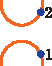
\includegraphics[scale=1]{CupCapDots.pdf}}}}}

\newcommand{\SigmaDotDot}{\mathord{\vcenter{\hbox{
\includegraphics[scale=1]{SigmaDotDot.pdf}}}}}
\newcommand{\SigmaDotDotExchange}{\mathord{\vcenter{\hbox{
\includegraphics[scale=1]{SigmaDotDotExchange.pdf}}}}}
\newcommand{\TwoLine}{\mathord{\vcenter{\hbox{
\includegraphics[scale=1]{TwoLine.pdf}}}}}
\newcommand{\TwoLineDots}{\mathord{\vcenter{\hbox{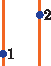
\includegraphics[scale=1]{TwoLineDots.pdf}}}}}

\newcommand{\RDotTwo}{\mathord{\vcenter{\hbox{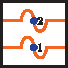
\includegraphics[scale=1]{RDotTwo.pdf}}}}}
\newcommand{\RDotTwoa}{\mathord{\vcenter{\hbox{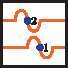
\includegraphics[scale=1]{RDotTwoa.pdf}}}}}
\newcommand{\RDotTwob}{\mathord{\vcenter{\hbox{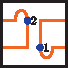
\includegraphics[scale=1]{RDotTwob.pdf}}}}}
\newcommand{\RDotTwoc}{\mathord{\vcenter{\hbox{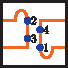
\includegraphics[scale=1]{RDotTwoc.pdf}}}}}

\newcommand{\FubeXXX}{\mathord{\vcenter{\hbox{
\includegraphics[scale=1]{EmptyTube.pdf}}}}}
\newcommand{\FubeXss}{\mathord{\vcenter{\hbox{
\includegraphics[scale=1]{OneLine.pdf}}}}}
\newcommand{\FubeXsds}{\mathord{\vcenter{\hbox{
\includegraphics[scale=1]{OneLineDot.pdf}}}}}

\newcommand{\AnnularTube}{\mathord{\vcenter{\hbox{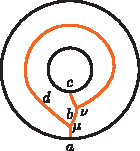
\includegraphics[scale=1]{AnnularTube.pdf}}}}}
\newcommand{\AnnularTubeNoIndex}{\mathord{\vcenter{\hbox{
\includegraphics[scale=1]{AnnularTubeNoIndex.pdf}}}}}

%\newcommand{\AnnulsLabel}[5]{\mathord{ \raisebox{.2ex}{$\scriptstyle{#2}$}\mkern2mu\overset{#3}{\underset{#4}{#1}}\mkern2mu\raisebox{0.2ex}{$\scriptstyle{#5}$} }}

\newcommand{\Annulusxprime}[2]{\mathord{\ooalign{
 \vphantom{\raisebox{1.3ex}{$\Big|^2$}}\cr\hidewidth
 \ensuremath{\scriptstyle{#2}}
 \hidewidth\cr 
 $\vcenter{\hbox{$#1$ }}$
 \cr\vphantom{ \raisebox{-1.3ex}{$\Big|_q$}} }}}

\newcommand{\AnnulsLabel}[5]{\mathord{ 
\mkern2mu\overset{#3}{{\Annulusxprime{#1}{#2}}}\mkern2mu\raisebox{0ex}{$\scriptstyle{#4}$} }}

%\newcommand{\AnnulsLabel}[5]{\mathord{ 
%\raisebox{.2ex}{$\scriptstyle{#2}$}\mkern2mu\overset{#3}{{#1}}\mkern2mu\raisebox{0.2ex}{$\scriptstyle{#5}$} }}

%\newcommand{\AnnulsLabel}[5]{\mathord{ 
%\raisebox{.2ex}{$\scriptstyle{#2}$}\mkern2mu\overset{#3}{{#1}}\mkern2mu\raisebox{0.2ex}{$\scriptstyle{#5}$} }}

%\newcommand{\Annulsx}[1]{{\mathord{\ooalign{ \vphantom{$\Big|^2$}\cr\hidewidth \ensuremath{#1}\hidewidth\cr$\vcenter{\hbox{
\includegraphics[scale=1]{AnnularTubeNoIndex.pdf}}}$\cr\vphantom{$\Big|_q$} }}}}		% Annulus with a spin structure label inside.
%
%\newcommand{\Annulsx}[1]{{\mathord{\ooalign{ \cr \hidewidth 
%{{\raisebox{1.2ex}{\hspace{1cm}$\scriptstyle{#1}$}}}
%\hidewidth\cr$\vcenter{\hbox{
\includegraphics[scale=1]{AnnularTubeNoIndex.pdf}}}$ }}}}		% Annulus with a spin structure label inside.

\newcommand{\Annulusx}[1]{{\mathord{\ooalign{ \vphantom{$\Big|^{\Big|^2}_{\Big|^2}$}\cr\hidewidth\ensuremath{#1}\hidewidth\cr$\vcenter{\hbox{
\includegraphics[scale=1]{AnnularTubeNoIndex.pdf}}}$\cr\vphantom{$\Big|_q$} }}}}		% BWbare with a symbol inside


%\newcommand{\Annulusx}[1]{{\mathord{\ooalign{ \vphantom{$\Big|^{\Big|}$} \cr \hidewidth 
%\raisebox{1ex}{$\scriptstyle{#1}$}
%\hidewidth\cr$\vcenter{\hbox{
\includegraphics[scale=1]{AnnularTubeNoIndex.pdf}}}$ }}}}		% Annulus with a spin structure label inside.


\newcommand{\AnTorusx}[2]{{\mathord{\ooalign{\vphantom{$\Big|^2$} \cr \hidewidth 
{\raisebox{-.5ex}{\hspace{1.8cm}$\scriptstyle{#2}$}}
\hidewidth\cr $\Annulusx{#1}$ }}}}		% Annulus with a spin structure label inside.

%\newcommand{\Vx}[1]{%
%  \ooalign{\Large $#1$\cr\hss\raisebox{1.4ex}{\scriptsize $x$}\hss}}
  
%\newcommand*{\Vx}{{ \AnnularTubeNoIndex }\kern0.2em\raisebox{1.4ex}{\tiny x}}


%\newcommand*{\Vx}{{ \AnnularTubeNoIndex }
%\kern-1.0em\raisebox{1.4ex}{ $\scriptstyle{x}$} \kern1.0em}
\newcommand*{\Annulus}[2]{{ #1 }
\kern-3.5em\raisebox{0ex}{ $\scriptstyle{#2}$} \kern3.5em} %Could change 0 to 1.2 to raise the B.

\newcommand*{\AnnulusP}[3]{{ \Annulus{#1}{#2} }
\kern-1.3em\raisebox{3.5ex}{ $\scriptstyle{#3}$} \kern1.3em} %Could change 0 to 1.2 to raise the B.


\newcommand{\FubesXs}{\mathord{\vcenter{\hbox{
\includegraphics[scale=1,angle=90,origin=c]{OneLine.pdf}}}}}
\newcommand{\FubesdXs}{\mathord{\vcenter{\hbox{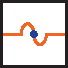
\includegraphics[scale=1]{FubesdXs.pdf}}}}}

\newcommand{\FubessX}{\mathord{\vcenter{\hbox{
\includegraphics[scale=1]{FubessX.pdf}}}}}
\newcommand{\FubessdX}{\mathord{\vcenter{\hbox{
\includegraphics[scale=1]{FubessdX.pdf}}}}}

\newcommand{\FubesXsa}{\mathord{\vcenter{\hbox{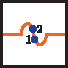
\includegraphics[scale=1]{FubesXsa.pdf}}}}}
\newcommand{\FubesXsb}{\mathord{\vcenter{\hbox{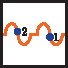
\includegraphics[scale=1]{FubesXsb.pdf}}}}}
\newcommand{\FubesXsc}{\mathord{\vcenter{\hbox{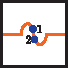
\includegraphics[scale=1]{FubesXsc.pdf}}}}}


\newcommand{\qqo}{\mathord{\vcenter{\hbox{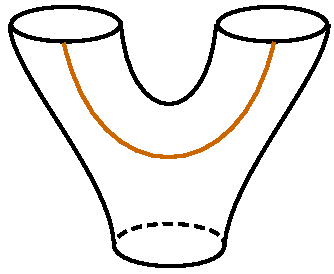
\includegraphics[scale=.4]{qq1.pdf}}}}}
\newcommand{\qtqo}{\mathord{\vcenter{\hbox{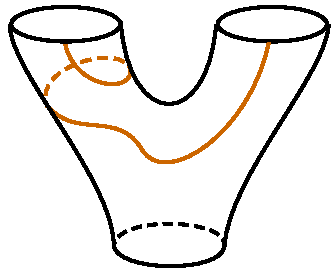
\includegraphics[scale=.4]{qtq1.pdf}}}}}
\newcommand{\qqto}{\mathord{\vcenter{\hbox{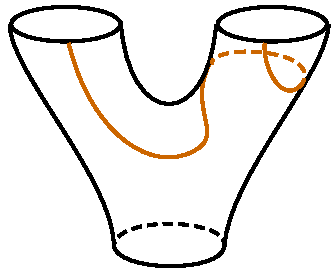
\includegraphics[scale=.4]{qqt1.pdf}}}}}
\newcommand{\qtqto}{\mathord{\vcenter{\hbox{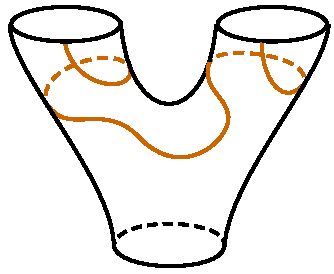
\includegraphics[scale=.4]{qtqt1.pdf}}}}}
\newcommand{\qqm}{\mathord{\vcenter{\hbox{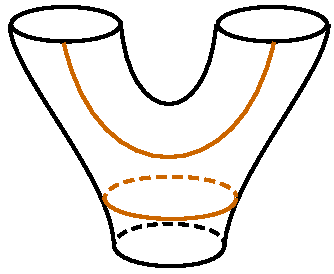
\includegraphics[scale=.4]{qqm.pdf}}}}}
\newcommand{\qtqm}{\mathord{\vcenter{\hbox{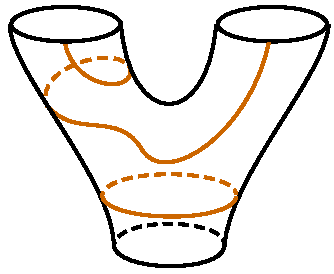
\includegraphics[scale=.4]{qtqm.pdf}}}}}
\newcommand{\qqtm}{\mathord{\vcenter{\hbox{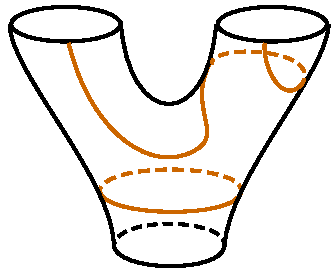
\includegraphics[scale=.4]{qqtm.pdf}}}}}
\newcommand{\qtqtm}{\mathord{\vcenter{\hbox{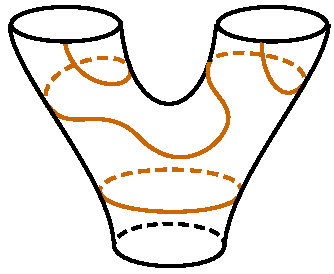
\includegraphics[scale=.4]{qtqtm.pdf}}}}}

\newcommand{\PantsPAP}{\mathord{\vcenter{\hbox{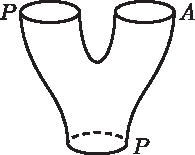
\includegraphics[scale=0.7]{PantsPAP.pdf}}}}}
\newcommand{\PantsPAsP}{\mathord{\vcenter{\hbox{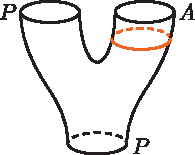
\includegraphics[scale=0.7]{PantsPAsP.pdf}}}}}

\newcommand{\PantsPsdAP}{\mathord{\vcenter{\hbox{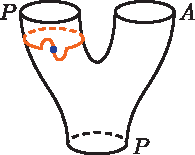
\includegraphics[scale=0.7]{PantsPsdAP.pdf}}}}}
\newcommand{\PantsPsdAsP}{\mathord{\vcenter{\hbox{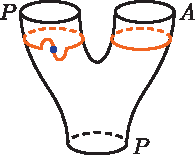
\includegraphics[scale=0.7]{PantsPsdAsP.pdf}}}}}



\newcommand{\PantsPPA}{\mathord{\vcenter{\hbox{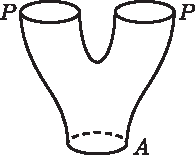
\includegraphics[scale=0.7]{PantsPPA.pdf}}}}}
\newcommand{\PantsPPAs}{\mathord{\vcenter{\hbox{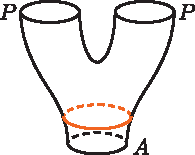
\includegraphics[scale=0.7]{PantsPPAs.pdf}}}}}

\newcommand{\PantsAsAshAsvt}{\mathord{\vcenter{\hbox{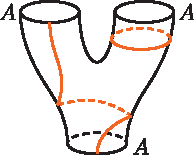
\includegraphics[scale=0.7]{PantsAsAshAsvt.pdf}}}}}
\newcommand{\PantsAstAAs}{\mathord{\vcenter{\hbox{\includegraphics[scale=0.7]{PantsAstAAs.pdf}}}}}

\newcommand{\PantsAstAshAs}{\mathord{\vcenter{\hbox{\includegraphics[scale=0.7]{PantsAstAshAs.pdf}}}}}
\newcommand{\PantsAsAshAs}{\mathord{\vcenter{\hbox{\includegraphics[scale=0.7]{PantsAsAshAs.pdf}}}}}
\newcommand{\PantsAsAAs}{\mathord{\vcenter{\hbox{\includegraphics[scale=0.7]{PantsAsAAs.pdf}}}}}

\newcommand{\Pantssvtsvtsh}{\mathord{\vcenter{\hbox{\includegraphics[scale=.7,origin=c]{Pantssvtsvtsh.pdf}}}}}
\newcommand{\Pantssvtsvsh}{\mathord{\vcenter{\hbox{\includegraphics[scale=.7,angle=0,origin=c]{Pantssvtsvsh.pdf}}}}}
\newcommand{\Pantssvsvtsh}{\mathord{\vcenter{\hbox{\includegraphics[scale=.7,angle=0,origin=c]{Pantssvsvtsh.pdf}}}}}
\newcommand{\Pantssvsvsh}{\mathord{\vcenter{\hbox{\includegraphics[scale=.7,angle=0,origin=c]{Pantssvsvsh.pdf}}}}}
\newcommand{\PantssvtsvtX}{\mathord{\vcenter{\hbox{\includegraphics[scale=.7,angle=0,origin=c]{PantssvtsvtX.pdf}}}}}
\newcommand{\PantssvtsvX}{\mathord{\vcenter{\hbox{\includegraphics[scale=.7,angle=0,origin=c]{PantssvtsvX.pdf}}}}}
%\newcommand{\PantssvtsvX}{\mathord{\vcenter{\hbox{\includegraphics[scale=.7,angle=0,origin=c]{PantssvtsvX.pdf}}}}}
\newcommand{\PantssvsvtX}{\mathord{\vcenter{\hbox{\includegraphics[scale=.7,angle=0,origin=c]{PantssvsvtX.pdf}}}}}
\newcommand{\PantssvsvX}{\mathord{\vcenter{\hbox{\includegraphics[scale=.7,angle=0,origin=c]{PantssvsvX.pdf}}}}}

\newcommand{\PantssvtXsvd}{\mathord{\vcenter{\hbox{\includegraphics[scale=.7,angle=0,origin=c]{PantssvtXsvd.pdf}}}}}
\newcommand{\Pantssvtshsvd}{\mathord{\vcenter{\hbox{\includegraphics[scale=.7,angle=0,origin=c]{Pantssvtshsvd.pdf}}}}}
\newcommand{\Pantssvshsvd}{\mathord{\vcenter{\hbox{\includegraphics[scale=.7,angle=0,origin=c]{Pantssvshsvd.pdf}}}}}
\newcommand{\PantssvXsvd}{\mathord{\vcenter{\hbox{\includegraphics[scale=.7,angle=0,origin=c]{PantssvXsvd.pdf}}}}}

\newcommand{\PantssvtXsvt}{\mathord{\vcenter{\hbox{\includegraphics[scale=.7,angle=0,origin=c]{PantssvtXsvt.pdf}}}}}
\newcommand{\PantssvXsvt}{\mathord{\vcenter{\hbox{\includegraphics[scale=.7,angle=0,origin=c]{PantssvXsvt.pdf}}}}}

\newcommand{\PantssvtXsv}{\mathord{\vcenter{\hbox{\includegraphics[scale=.7,angle=0,origin=c]{PantssvtXsv.pdf}}}}}

\newcommand{\PantssvXsv}{\mathord{\vcenter{\hbox{\includegraphics[scale=1,angle=0,origin=c]{PantssvXsv.pdf}}}}}

\newcommand{\TwoLinedotdot}{\mathord{\vcenter{\hbox{\includegraphics[scale=1.5,angle=0,origin=c]{TwoLinedotdot.pdf}}}}}

\newcommand{\Id}{\mathord{\vcenter{\hbox{\includegraphics[scale=1.5,angle=0,origin=c]{Id.pdf}}}}}

\newcommand{\CupSigmadot}{\mathord{\vcenter{\hbox{\includegraphics[scale=1.5,angle=0,origin=c]{Cupdot.pdf}}}}}

\newcommand{\CupSigma}{\mathord{\vcenter{\hbox{\includegraphics[scale=1.5,angle=0,origin=c]{Cup.pdf}}}}}

\newcommand{\StaggaredGSOdd}{\mathord{\vcenter{\hbox{\includegraphics[scale=1.5,angle=0,origin=c]{StaggaredGSOdd.pdf}}}}}
\newcommand{\StaggaredGSEven}{\mathord{\vcenter{\hbox{\includegraphics[scale=1.5,angle=0,origin=c]{StaggeredGSEven.pdf}}}}}

\newcommand{\StaggaredGSEvenR}{\mathord{\vcenter{\hbox{\reflectbox{\includegraphics[scale=1.5,angle=0,origin=c]{StaggeredGSEven.pdf}}}}}}





\newcommand{\VxsdsY}{\mathord{\vcenter{\hbox{\includegraphics[scale=0.3,angle=0,origin=c]{Vxsds.pdf}}}}}
\newcommand{\VsdxsY}{\mathord{\vcenter{\hbox{\includegraphics[scale=0.3,angle=0,origin=c]{Vsdxs.pdf}}}}}
\newcommand{\VtssdxY}{\mathord{\vcenter{\hbox{\includegraphics[scale=0.3,angle=0,origin=c]{Vtssdx.pdf}}}}}

\newcommand{\Vssdx}{\mathord{\vcenter{\hbox{\includegraphics[scale=0.3,angle=0,origin=c]{Vssdx.pdf}}}}}
\newcommand{\Vxsds}{\mathord{\vcenter{\hbox{\reflectbox{\includegraphics[scale=0.3,angle=0,origin=c]{Vssdx.pdf}}}}}}

\newcommand{\Vssx}{\mathord{\vcenter{\hbox{\includegraphics[scale=0.3,angle=0,origin=c]{Vssx.pdf}}}}}
\newcommand{\Vxss}{\mathord{\vcenter{\hbox{\reflectbox{\includegraphics[scale=0.3,angle=0,origin=c]{Vssx.pdf}}}}}}

\newcommand{\Vsxs}{\mathord{\vcenter{\hbox{\includegraphics[scale=0.3,angle=0,origin=c]{Vsxs.pdf}}}}}
\newcommand{\Vsxsd}{\mathord{\vcenter{\hbox{\includegraphics[scale=0.3,angle=0,origin=c]{Vsxsd.pdf}}}}}

\newcommand{\VsxsY}{\mathord{\vcenter{\hbox{\includegraphics[scale=0.3,angle=180,origin=c]{Vsxs.pdf}}}}}
\newcommand{\VssxY}{\mathord{\vcenter{\hbox{\includegraphics[scale=0.3,angle=180,origin=c]{Vssx.pdf}}}}}
\newcommand{\VxssY}{\mathord{\vcenter{\hbox{\reflectbox{\includegraphics[scale=0.3,angle=180,origin=c]{Vssx.pdf}}}}}}

\newcommand{\PsiFermion}{\mathord{\vcenter{\hbox{\includegraphics[scale=1.5]{PsiFermion.pdf}}}}}
\newcommand{\PsiFermionTwist}{\mathord{\vcenter{\hbox{\includegraphics[scale=1.5]{PsiFermionTwist.pdf}}}}}

\newcommand{\TwoFermion}{\mathord{\vcenter{\hbox{\includegraphics[scale=1.5]{TwoFermion.pdf}}}}}
\newcommand{\TwoFermionExchange}{\mathord{\vcenter{\hbox{\includegraphics[scale=1.5]{TwoFermionExchange.pdf}}}}}


\newcommand{\Spin}{\mathord{\vcenter{\hbox{\includegraphics[scale=1.5]{Spin.pdf}}}}}
\newcommand{\PsiIdentity}{\mathord{\vcenter{\hbox{\includegraphics[scale=1.5]{PsiIdentity.pdf}}}}}

\newcommand{\TwoPsiExchange}{\mathord{\vcenter{\hbox{\includegraphics[scale=1.5]{TwoPsiExchange.pdf}}}}}
\newcommand{\TwoPsiIdentity}{\mathord{\vcenter{\hbox{\includegraphics[scale=1.5]{TwoPsiIdentity.pdf}}}}}


\newcommand{\PsiEnd}{\mathord{\vcenter{\hbox{\includegraphics[scale=1.5]{PsiEnd.pdf}}}}}
\newcommand{\PsiEndExchange}{\mathord{\vcenter{\hbox{\includegraphics[scale=1.5]{PsiEndExchange.pdf}}}}}

\newcommand{\DotSlidea}{\mathord{\vcenter{\hbox{\includegraphics[scale=1]{DotSlidea.pdf}}}}}
\newcommand{\DotSlideb}{\mathord{\vcenter{\hbox{\includegraphics[scale=1]{DotSlideb.pdf}}}}}
\newcommand{\DotSlidec}{\mathord{\vcenter{\hbox{\includegraphics[scale=1]{DotSlidec.pdf}}}}}
\newcommand{\DotSlided}{\mathord{\vcenter{\hbox{\includegraphics[scale=1]{DotSlided.pdf}}}}}

\newcommand{\QCapDotL}{\mathord{\vcenter{\hbox{\includegraphics[scale=1]{QDotslide.pdf}}}}}
\newcommand{\QCupDotR}{\mathord{\vcenter{\hbox{\includegraphics[scale=1,angle=180,origin=c]{QDotslide.pdf}}}}}
\newcommand{\QCapDotR}{\mathord{\vcenter{\hbox{\reflectbox{\includegraphics[scale=1]{QDotslide.pdf}}}}}}
\newcommand{\QCupDotL}{\mathord{\vcenter{\hbox{\reflectbox{\includegraphics[scale=1,angle=180,origin=c]{QDotslide.pdf}}}}}}

\newcommand{\TwodotCap}{\mathord{\vcenter{\hbox{\includegraphics[scale=1]{TwodotCap.pdf}}}}}
\newcommand{\TwodotCup}{\mathord{\vcenter{\hbox{\includegraphics[scale=1]{TwodotCup.pdf}}}}}


\newcommand{\Bpa}{\mathord{\vcenter{\hbox{\includegraphics[scale=1]{Bpa.pdf}}}}}
\newcommand{\Bpb}{\mathord{\vcenter{\hbox{\includegraphics[scale=1]{Bpb.pdf}}}}}
\newcommand{\Bpc}{\mathord{\vcenter{\hbox{\includegraphics[scale=1]{Bpc.pdf}}}}}
\newcommand{\Bpd}{\mathord{\vcenter{\hbox{\includegraphics[scale=1]{Bpd.pdf}}}}}
\newcommand{\Bpe}{\mathord{\vcenter{\hbox{\includegraphics[scale=1]{Bpe.pdf}}}}}
\newcommand{\Bpf}{\mathord{\vcenter{\hbox{\includegraphics[scale=1]{Bpf.pdf}}}}}
\newcommand{\Bpg}{\mathord{\vcenter{\hbox{\includegraphics[scale=1]{Bpg.pdf}}}}}
\newcommand{\Bph}{\mathord{\vcenter{\hbox{\includegraphics[scale=1]{Bph.pdf}}}}}
\newcommand{\Bpi}{\mathord{\vcenter{\hbox{\includegraphics[scale=1]{Bpi.pdf}}}}}

\newcommand{\LocalRelationLeft}{\mathord{\vcenter{\hbox{\includegraphics[scale=1]{LocalRelationLeft.pdf}}}}}
\newcommand{\LocalRelationRight}{\mathord{\vcenter{\hbox{\includegraphics[scale=1]{LocalRelationRight.pdf}}}}}
\newcommand{\LocalRelationUp}{\mathord{\vcenter{\hbox{\includegraphics[scale=1]{LocalRelationUp.pdf}}}}}
\newcommand{\LocalRelationDown}{\mathord{\vcenter{\hbox{\includegraphics[scale=1]{LocalRelationDown.pdf}}}}}

\newcommand{\PlaquettePrime}{\mathord{\vcenter{\hbox{\includegraphics[scale=1]{PlaquettePrime.pdf}}}}}

\newcommand{\ycenter}{\mathord{\vcenter{\hbox{\includegraphics[scale=1.3]{ycenter.pdf}}}}}
\newcommand{\ex}{\mathord{\vcenter{\hbox{\includegraphics[scale=1.3]{ex.pdf}}}}}
\newcommand{\ey}{\mathord{\vcenter{\hbox{\includegraphics[scale=1.3]{ey.pdf}}}}}
\newcommand{\eone}{\mathord{\vcenter{\hbox{\includegraphics[scale=1.3]{eone.pdf}}}}}

\newcommand{\TubeXb}{\mathord{\vcenter{\hbox{\includegraphics[scale=1]{TubeXb.pdf}}}}}
\newcommand{\TubeXa}{\mathord{\vcenter{\hbox{\includegraphics[scale=1]{TubeXa.pdf}}}}}
\newcommand{\TubeXtwist}{\mathord{\vcenter{\hbox{\includegraphics[scale=1]{TubeXtwist.pdf}}}}}
\newcommand{\Tubeidx}{\mathord{\vcenter{\hbox{\includegraphics[scale=1]{Tubeidx.pdf}}}}}
\newcommand{\Tubexloop}{\mathord{\vcenter{\hbox{\includegraphics[scale=1]{Tubexloop.pdf}}}}}
\newcommand{\TubeEmpty}{\mathord{\vcenter{\hbox{\includegraphics[scale=1]{TubeEmpty.pdf}}}}}

\newcommand{\xOdd}{\mathord{\vcenter{\hbox{\includegraphics[scale=1]{xOdd.pdf}}}}}
\newcommand{\tOdd}{\mathord{\vcenter{\hbox{\includegraphics[scale=1]{tOdd.pdf}}}}}
\newcommand{\vOdd}{\mathord{\vcenter{\hbox{\includegraphics[scale=1]{vOdd.pdf}}}}}
\newcommand{\hOdd}{\mathord{\vcenter{\hbox{\includegraphics[scale=1]{hOdd.pdf}}}}}

\newcommand{\TorusBasisa}{\mathord{\vcenter{\hbox{\includegraphics[scale=1]{TorusBasisa.pdf}}}}}
\newcommand{\TorusBasisb}{\mathord{\vcenter{\hbox{\includegraphics[scale=1]{TorusBasisb.pdf}}}}}
\newcommand{\STorusBasisa}{\mathord{\vcenter{\hbox{\includegraphics[scale=1]{STorusBasisa.pdf}}}}}

\newcommand{\scale}{}

\newcommand{\TubeXbv}{\mathord{\vcenter{\hbox{\includegraphics[scale=1]{TubeXbv.pdf}}}}}
\newcommand{\TubeXav}{\mathord{\vcenter{\hbox{\includegraphics[scale=1]{TubeXav.pdf}}}}}
\newcommand{\TubeXtwistv}{\mathord{\vcenter{\hbox{\includegraphics[scale=1]{TubeXtwistv.pdf}}}}}
\newcommand{\Tubeidxv}{\mathord{\vcenter{\hbox{\includegraphics[scale=1]{Tubeidxv.pdf}}}}}
\newcommand{\TubeEmptyv}{\mathord{\vcenter{\hbox{\includegraphics[scale=1]{TubeEmptyv.pdf}}}}}



\newcommand{\TorusQQQa}{\mathord{\vcenter{\hbox{\includegraphics[scale=1]{TorusQQQa.pdf}}}}}
\newcommand{\TorusQQQb}{\mathord{\vcenter{\hbox{\includegraphics[scale=1]{TorusQQQb.pdf}}}}}
\newcommand{\TorusQQQc}{\mathord{\vcenter{\hbox{\includegraphics[scale=1]{TorusQQQc.pdf}}}}}
\newcommand{\TorusQQQd}{\mathord{\vcenter{\hbox{\includegraphics[scale=1]{TorusQQQd.pdf}}}}}

\newcommand{\VSa}{\mathord{\vcenter{\hbox{\includegraphics[scale=1.3]{VSa.pdf}}}}}
\newcommand{\VSb}{\mathord{\vcenter{\hbox{\includegraphics[scale=1.3]{VSb.pdf}}}}}
\newcommand{\VSc}{\mathord{\vcenter{\hbox{\includegraphics[scale=1.3]{VSc.pdf}}}}}
\newcommand{\VSd}{\mathord{\vcenter{\hbox{\includegraphics[scale=1.3]{VSd.pdf}}}}}


\newcommand{\Vxyxxa}{\mathord{\vcenter{\hbox{\includegraphics[scale=1.3]{Vxyxxa.pdf}}}}}
\newcommand{\Vxyxxb}{\mathord{\vcenter{\hbox{\includegraphics[scale=1.3]{Vxyxxb.pdf}}}}}
\newcommand{\Vyxxxa}{\mathord{\vcenter{\hbox{\includegraphics[scale=1.3]{Vyxxxa.pdf}}}}}
\newcommand{\Vyxxxb}{\mathord{\vcenter{\hbox{\includegraphics[scale=1.3]{Vyxxxb.pdf}}}}}
\newcommand{\Vxxyxa}{\mathord{\vcenter{\hbox{\includegraphics[scale=1.3]{Vxxyxa.pdf}}}}}
\newcommand{\Vxxyxb}{\mathord{\vcenter{\hbox{\includegraphics[scale=1.3]{Vxxyxb.pdf}}}}}

\newcommand{\Vxxxa}{\mathord{\vcenter{\hbox{\includegraphics[scale=1.3]{Vxxxa.pdf}}}}}


\newcommand{\Vxxxya}{\mathord{\vcenter{\hbox{\includegraphics[scale=1.3]{Vxxxya.pdf}}}}}
\newcommand{\Vxxxyb}{\mathord{\vcenter{\hbox{\includegraphics[scale=1.3]{Vxxxyb.pdf}}}}}

\newcommand{\Vxxxva}{\mathord{\vcenter{\hbox{\includegraphics[scale=1.3]{Vxxxva.pdf}}}}}
\newcommand{\Vxxxvb}{\mathord{\vcenter{\hbox{\includegraphics[scale=1.3]{Vxxxvb.pdf}}}}}

\newcommand{\VSeven}{\mathord{\vcenter{\hbox{\includegraphics[scale=1.3]{VSeven.pdf}}}}}

\newcommand{\Vrhorhorhoodd}{\mathord{\vcenter{\hbox{\includegraphics[scale=1.3]{Vrhorhorhoodd.pdf}}}}}
\newcommand{\Vrhorhorho}{\mathord{\vcenter{\hbox{\includegraphics[scale=1.3]{Vrhorhorho.pdf}}}}}
\newcommand{\PivotEsixOdd}{\mathord{\vcenter{\hbox{\includegraphics[scale=1.3]{PivotE6Odd.pdf}}}}}
\newcommand{\PivotEsixEven}{\mathord{\vcenter{\hbox{\includegraphics[scale=1.3]{PivotE6even.pdf}}}}}
 
 \newcommand{\EsixDynkin}{\mathord{\vcenter{\hbox{\includegraphics[scale=1]{EsixDynkin.pdf}}}}}
 \newcommand{\EsixCondensePsi}{\mathord{\vcenter{\hbox{\includegraphics[scale=1]{EsixCondensePsi.pdf}}}}}
 
 \newcommand{\halfesix}{\frac{1}{2}\text{E}_6}
 \newcommand{\SphereTube}{\mathord{\vcenter{\hbox{\includegraphics[scale=1.5]{SphereTube.pdf}}}}}
  \newcommand{\SphereTubeTube}{\mathord{\vcenter{\hbox{\includegraphics[scale=1.5]{SphereTubeTube.pdf}}}}}
    \newcommand{\TubeMultiplyTopCoefficent}{\mathord{\vcenter{\hbox{\includegraphics[scale=1.5]{TubeMultiplyTopCoefficent.pdf}}}}}
        \newcommand{\TubeMultiplyBottomCoefficient}{\mathord{\vcenter{\hbox{\includegraphics[scale=1.5]{TubeMultiplyBottomCoefficient.pdf}}}}}
  
 \newcommand{\TTorus}{\mathord{\vcenter{\hbox{\includegraphics[scale=1]{TTorus.pdf}}}}}
 

\newcommand{\Idx}{\mathord{\vcenter{\hbox{\includegraphics[scale=1.3]{Idx.pdf}}}}}
\newcommand{\Idy}{\mathord{\vcenter{\hbox{\includegraphics[scale=1.3]{Idy.pdf}}}}}
\newcommand{\Kappay}{\mathord{\vcenter{\hbox{\includegraphics[scale=1.3]{Kappay.pdf}}}}}
\newcommand{\Kappax}{\mathord{\vcenter{\hbox{\includegraphics[scale=1.3]{Kappax.pdf}}}}}

\newcommand{\Vxxy}{\mathord{\vcenter{\hbox{\includegraphics[scale=1.3]{Vxxy.pdf}}}}}
\newcommand{\Vxxydual}{\mathord{\vcenter{\hbox{\includegraphics[scale=1.3]{Vxxydual.pdf}}}}}

\newcommand{\xxypivota}{\mathord{\vcenter{\hbox{\includegraphics[scale=1.3]{xxypivota.pdf}}}}}
\newcommand{\xxypivotb}{\mathord{\vcenter{\hbox{\includegraphics[scale=1.3]{xxypivotb.pdf}}}}}
\newcommand{\xxypivotadual}{\mathord{\vcenter{\hbox{\includegraphics[scale=1.3]{xxypivotadual.pdf}}}}}
\newcommand{\xxypivotbdual}{\mathord{\vcenter{\hbox{\includegraphics[scale=1.3]{xxypivotbdual.pdf}}}}}


\newcommand{\Vyxxdual}{\mathord{\vcenter{\hbox{\includegraphics[scale=1.3]{Vyxxdual.pdf}}}}}
\newcommand{\yxxpivotbdual}{\mathord{\vcenter{\hbox{\includegraphics[scale=1.3]{yxxpivotbdual.pdf}}}}}
\newcommand{\yxxpivotadual}{\mathord{\vcenter{\hbox{\includegraphics[scale=1.3]{yxxpivotadual.pdf}}}}}
\newcommand{\Vxyxdual}{\mathord{\vcenter{\hbox{\includegraphics[scale=1.3]{Vxyxdual.pdf}}}}}
\newcommand{\xyxpivotbdual}{\mathord{\vcenter{\hbox{\includegraphics[scale=1.3]{xyxpivotbdual.pdf}}}}}
\newcommand{\xyxpivotadual}{\mathord{\vcenter{\hbox{\includegraphics[scale=1.3]{xyxpivotadual.pdf}}}}}
\newcommand{\Vyxx}{\mathord{\vcenter{\hbox{\includegraphics[scale=1.3]{Vyxx.pdf}}}}}
\newcommand{\yxxpivotb}{\mathord{\vcenter{\hbox{\includegraphics[scale=1.3]{yxxpivotb.pdf}}}}}
\newcommand{\yxxpivota}{\mathord{\vcenter{\hbox{\includegraphics[scale=1.3]{yxxpivota.pdf}}}}}
\newcommand{\Vxyx}{\mathord{\vcenter{\hbox{\includegraphics[scale=1.3]{Vxyx.pdf}}}}}
\newcommand{\xyxpivotb}{\mathord{\vcenter{\hbox{\includegraphics[scale=1.3]{xyxpivotb.pdf}}}}}
\newcommand{\xyxpivota}{\mathord{\vcenter{\hbox{\includegraphics[scale=1.3]{xyxpivota.pdf}}}}}







%%% if we want to leave a secret message
%\usepackage[pdftex, bookmarks={false}, pdftitle={Super lattice models}]{hyperref}
%%%

\begin{document}


\title{Fermion condensation and super lattices models}
\author{David Aasen, Ethan Lake, Kevin Walker, and Zhenghan Wang}
%\affiliation{Department of Physics and Astronomy, University of Utah, Salt Lake City, UT 84112, USA}
%\emailAdd{lake@physics.utah.edu}

\date{\today}

\maketitle

%\tableofcontents
\begin{abstract}
- fermion condensation/ Ising example

- modular transformations

- super-pivotal category

- exactly solvable Hamiltonian
\end{abstract}

\tableofcontents




\section{Introduction}

\begin{itemize}
\item fermion condensation as a method to generate super-pivotal categories
\item explain relations to previous work. 
\item emphasize tensoring over endo-morphisms
\item mention string nets from tubes/excitations
\end{itemize}




\section{Fermion condensation in the Ising TQFT}

Before discussing super pivotal categories in the abstract and general techniques for constructing examples thereof,
we will give a detailed account of one of the simplest examples:
the $C_2$ super pivotal category.
This theory 
\kw{I can't decide whether to call these ``categories" or ``TQFTs" or ``theories"; maybe use all three terms.}
is obtained from the Ising TQFT by condensing the emergent fermion $\psi$, as described below.
\kw{need to revisit this, since there will be at least some general discussion of condensation in this section}

\kwsep

Older outline:

\begin{itemize}
\item Here we explain how to quotient by the fermion in the Ising TQFT. 
\item condense fermions
\item explain inconsistencies that necessitate spin structure, give physical interpretation of $p+ip$ SC.
\item define spin structure and show why it's a phase of fermions. Mention that condensing $\psi$ couples the fermions and the Ising theory together 
\item graphical calculus of condensed theory --- the constraint on $A^4$, how boxes work, moving dots around is $A^4$ from unitarity, etc
\item give explicit example of why it's important to tensor over endomorphisms (e.g. getting endo space right)
\item Drinfeld center of condensed theory: can briefly mention physical picture for why tubing (fubing?) works, talk about how this gets enlarged with spin stuff. Work through the identifications of each sector with the Clifford algebras 
\item oddly isomorphic particles
\item Fusion of quasi-particles --- include some (one or two?) examples of fusion spaces and how we do the calculation. 
\item braiding of quasi-particles 
\item modular transformations/relation to braiding data, filling in $S^3$, getting S matrix for all spin structures, philosophy about well-definedness of $S$ and $T$. 
\item state sum???
\end{itemize}



\subsection{Ising TQFT} \ethan{will be easy to finish later}
Here we introduce the Ising TQFT via Kauffamann and Lins\cite{Lins1994}. 
We choose $A = e^{\frac{2 \pi i}{16}}$, a primitive 16th root of unity. 
\kw{This contradicts $A = \pm ie^{\pm i\pi/8}$ below; perhaps just leave $A$ as an undetermined
primitive 16th root of 1.}
We label the identity particle $1$, Ising anyon $\sigma$ and the fermion $\psi$.
The quantum dimensions are
\be
d_1 = 1 \quad d_\sigma = -A^2 - A^{-2} \quad d_\psi =1 
\ee
The four different choices $A = \pm ie^{\pm i\pi/8}$ all give us positive quantum dimensions $d = \sqrt{2}$. 
\dave{will come back to this.}

\medskip

\kw{draw attention to the facts that (1) $\phi$ is not transparent, (2) $\psi$ has twist $-1$, 
and (3) $\psi$ has fermionic statistics}






\newcommand{\braid}{\mathord{\vcenter{\hbox{\includegraphics[scale=1.5]{braid.pdf}}}}}
\newcommand{\TLIdentity}{\mathord{\vcenter{\hbox{\includegraphics[scale=1.5]{TLIdentity.pdf}}}}}
\newcommand{\TemperleyLieb}{\mathord{\vcenter{\hbox{\includegraphics[scale=1.5]{TemperleyLieb.pdf}}}}}
  
\begin{align}
\braid = A\;  \TemperleyLieb \; +\;  A^{-1}\;  \TLIdentity
\end{align}

\begin{figure}
\includegraphics{folding_A3.pdf}
\caption{Performing the condensation from the Ising theory to the $C_2$ theory. The Dynkin diagram for $A_3$ folds about the node labeled by $\sigma$, producing the Dynkin diagram 
for $C_2$. The first node in the $C_2$ Dynkin diagram is the (fermionic) vacuum, and the second node is $\beta$, the image of $\sigma$ under condensation.
\kw{Scott and I use the convention that q-type particles in the principal graph get a double circle, and lines connecting
m-type and q-type particles are doubled, with arrow pointing to the m-type particle.}
\kw{let's put this figure later in this section}
} 
\end{figure}



\subsection{Condensation in general}

Let $\mcc$ be a ribbon category and let $\alpha$ be a particle (simple object) of $\mcc$ which we hope to condense.
In category theoretic terms, we want to add morphisms to $\mcc$ so that $\alpha$ becomes
isomorphic to the trivial particle $\unit$ (or, more generally, to a direct sum of several copies of $\unit$). 
We can think of this as a categorical quotient, with result denoted $\mcc/\langle \alpha \cong \unit \rangle$ or
more simply $\mcc/\alpha$.

In our graphical calculus, condensing $\alpha$ means that $\alpha$ worldlines are allowed to have endpoints at locations where they are ``absorbed'' into the condensate. 
We will mark the locations where $\alpha$ particles are absorbed into the condensate with boxes:
\begin{align}
\label{box_def}
\alpha\; \PsiFermion\; , 
\end{align}
where the horizontal blue line is an $\alpha$ worldline. 
For simplicity, we will assume that $\alpha\otimes\alpha\cong \unit$ (which will be true in the examples considered in this paper), 
although most of the following discussion works more generally.

In order for this condensation procedure to not cause unintended collapse in $\mcc$,
$\alpha$ must satisfy three conditions:

\begin{itemize}

\item First, $\alpha$ must have the spin of a boson: that is, the twist of $\alpha$ must be 1.
This is because
\be 
\label{twist_inconsistency} \PsiFermion = \PsiFermionTwist = \theta_\alpha \ \PsiFermion\;,
\ee
and so if $\theta_\alpha \neq 1$, diagrams in which $\alpha$ worldlines are absorbed into the condensate are identically zero, and condensation is impossible. 

\item Secondly, $\alpha$ must be statistically bosonic, i.e. it must braid trivially with itself.  
To see this, we make the following manipulations:
\be \label{statistics_inconsistency}
\mathord{\vcenter{\hbox{\includegraphics[scale=1.5]{TwoFermion_nolabels.pdf}}}} = \ \mathord{\vcenter{\hbox{\includegraphics[scale=1.5]{TwoFermionExchange_nolabels.pdf}}}} = \theta_{\alpha,\alpha} \mathord{\vcenter{\hbox{\includegraphics[scale=1.5]{TwoFermion_nolabels.pdf}}}},\ee
where $\theta_{\alpha,\alpha}$ is the self-statistics of $\alpha$. 
By the spin-statistics relation this condition is not independent of the previous one, but it will be useful to regard them as separate constraints for the purpose of the fermion condensation procedure described in the next section\footnote{If we drop positivity requirements, we can violate the spin-statistics theorem and have particles which are fermionic in spin but not statistics or vice-versa; see [Scott and Kevin's paper] for a discussion of this.}. 

\item Finally, 
$\alpha$ must braid trivially with every particle in $\mcc$. In category-theoretic language, this means that $\alpha$ must lie in the transparent subcategory of $\mcc$.
If a particle $\beta$ braids non-trivially with $\alpha$ (i.e.\ if the left and right braidings are not equal),
then any string diagram which includes a $\beta$ particle must be zero: (we assume the quantum dimension of alpha is one for convenience)
\be\label{transparency_inconsistency} 
\mathord{\vcenter{\hbox{\includegraphics[scale=1]{alphabox_beta_braiding.pdf}}}},
\ee
where the orange line is a $\beta$ worldline and $\theta_{\alpha,\beta}$ is the mutual statistics of $\alpha$ and $\beta$. 
The first two equalities follow from the fact that the location of a particle being absorbed into the condensate is not physically significant: no operator can distinguish between states that differ only by the location of an $\alpha$ endpoint. 
Therefore, if $\theta_{\alpha,\beta}\neq1$, condensing $\alpha$ causes unintended collapse in $\mcc$, since it confines $\beta$. 
\end{itemize}

To summarize, in order to condense $\alpha$, $\alpha$ must have a twist of 1, bosonic self-statistics, and must braid trivially with every other particle in the theory. 
If any of these conditions are violated, we
will have to work harder to construct $\mcc/\alpha$.



%%%%%%%%%%%%%%%%%%%%%%%%%%%%%%%
\subsection{Condensing $\psi$ in Ising \ethan{in progress}} \label{condensing_psi}
%%%%%%%%%%%%%%%%%%%%%%%%%%%%%%%

In this subsection we describe our procedure for condensing $\psi$ in the Ising theory. 
We would like to ``condense" the $\psi$ particle by constructing the quotient theory $\mcc / \psi$. We will denote the condensed theory by $C_2$, for reasons that we will elaborate on later, and we will denote the image of $\sigma$ under the condensation process as $\beta$.

First, we note that $\psi$ is fermionic in both spin and statistics,
\begin{align} \label{psi_a_fermion}
\Spin = (-1) \times  \PsiIdentity
\qquad \qquad \TwoPsiExchange =  (-1) \times\TwoPsiIdentity.
\end{align}
Additionally, $\psi$ has nontrivial braiding with $\beta$, and as such $\psi$ is not transparent. This means that If we perform unrestricted condensation on $\psi$, $\beta$ worldlines are confined, since
\be \label{box_beta_nowall_braiding}
\mathord{\vcenter{\hbox{\includegraphics[scale=1]{box_beta_nowall_braiding.pdf}}}}.\ee
Thus, $\psi$ violates all three of the conditions that particles in a condensate must satisfy! 
To condense $\psi$, we will clearly need some additional help. 

We will first examine how to address the non-transparency of $\psi$. As we saw above in \eqref{box_beta_nowall_braiding}, we can't allow world lines of $\psi$ to disappear anywhere
in the 3-dimensional space-time.
However, if we restrict the $\psi$ worldline endpoints to a 2-dimensional subset of the boundary of 3-dimensional spacetime,
we {\it can} obtain a consistent graphical calculus.
In this paper, we will adopt the convention that $\psi$ world lines are allowed to terminate on a codimension-1 ``back wall", located on a spatial boundary of the system that is located ``behind'' all other world lines drawn in our graphical calculus. 

Figure \ref{backwall} (a) demonstrates this graphically, with the light blue back section of the box denoting the back wall, on which the $\psi$ worldlines can be absorbed. 
String-net graphs in our (2+1)D spacetime can be reduced to string-net graphs in (1+1)D spacetime by introducing a shorthand notation for $\psi$-lines terminating on the back wall. This notation is shown in Figure \ref{backwall} (b), where we use boxes to denote places where $\psi$ worldlines head straight back into the back wall and terminate.

The ``back wall'' condensation process ``transparentizes'' $\psi$, and allows us to condense $\psi$ without confining $\beta$. Indeed, we have 
\be \label{box_beta_braiding}
\mathord{\vcenter{\hbox{\includegraphics[scale=1]{box_beta_braiding.pdf}}}},\ee
where we have performed an $F$-move to obtain the second equality. 
\ethan{I guess I still don't understand why this means the theory isn't braided: we can move endpoints over $\beta$ lines if we want.}

An important consequence of the existence of the back wall this is that the quotient category $C_2$ is not braided, as it maps onto a (1+1)D theory. In category theoretic terms, the condensation process takes a 3-category (braided category) to a 2-category (tensor category)\footnote{The condensed theory does however retain a ``front braiding" by the Ising category, so it is more than a mere tensor category.}.

A useful picture for this condensation process is to imagine the existence of a codimenion-1 ``back wall'' that plays the role of the condensate. In this picture, we interpret the boxes at the endpoints of $\psi$ lines as marking the location where $\psi$ lines meet the back wall. The back wall carries a spin structure to provide the minus signs that make equations \eqref{boxspin} and \eqref{boxbraid} hold. This point of view allows us to interpret the condensation procedure as a form of dimensional reduction. For example, when condensing the fermion in the Ising TQFT, we can think of the condensation procedure as a map from the (2+1)D Ising theory to the (1+1)D $C_2$ theory. The fact that the Ising theory looses a dimension upon condensation is roughly equivalent to the statement that the Ising theory is a {\it braided} modular tensor category, but the $C_2$ theory is not: the condensation process destroys the braided structure.\footnote{This is similar to the relationship between a (1+1)D phase described by the tensor category $\mcc$ and the (2+1)D phase described by the braided category $\mcz(\mcc)$.}
%This is because the spin structure ocurrs along on a two dimensional surface embedded in the TQFT. \ethan{I'm not sure how true this is}

\begin{figure}
  \centering
    \includegraphics{Backwall_figure.pdf}
      \caption{\label{backwall} (a) The ``back wall'' picture. The box represents a section of a (2+1)D Ising TQFT, with the codimension-1 back wall indicated by the blue back side of the box. $\psi$ worldlines to be absorbed into the back wall at marked points labelled by $1,2,3,4$. Free $\psi$ endpoints which do not terminate on the back wall are not allowed. (b) Our way of representing the picture (a) in a (1+1)D graphical calculus. We have squashed the box down to a two dimensional plane, with the blue boxes representing the points at which the $\psi$ lines ``go straight back and hit the back wall''.}
\end{figure}



The back wall construction ``transparentizes'' $\psi$, fixing the inconsistency presented by \eqref{transparency_inconsistency}. 
However, we have not yet addressed the spin and statistics inconsistencies \eqref{twist_inconsistency} and \eqref{statistics_inconsistency}.

To fix the twist inconsistency \eqref{twist_inconsistency}, we will equip the theory with a spin structure. Loosely, the idea is to couple the $\psi$ endpoints to a spin structure, which ``bosonizes'' them and allows the condensation procedure to go through. 
This amounts to adding a phase of {\it physical} (not anyonic or emergent) fermions to the theory, and attaching a single physical fermion to each $\psi$ endpoint. 
This fixes the spin inconsistency \eqref{spin_inconsistency}, since rotating the physical fermion on the $\psi$ endpoint by $2\pi$ gives an extra factor of $-1$:
\begin{align} \label{boxspin}
\PsiFermion = (-1)\ \PsiFermionTwist = (-1)^2\ \PsiFermion. 
\end{align}

To satisfy the statistical constraint \eqref{statistics_inconsistency}, we will add Kozul signs supervector spaces...Finally, the fact that $\psi$ has fermionic statistics forces our vector spaces to be super vector spaces,
which Koszul signs to keep track of signs related to the ordering of $\psi$ endpoints.

Adding fermions to the $\psi$ endpoints means that we have to keep track of their normal ordering, since permuting two $\psi$ endpoints must come at the expense of a minus sign. 
This means that the exchange of two labeled $\psi$ endpoints is bosonic, in that 
\begin{align} \label{boxbraid}
\TwoFermion =\ \TwoFermionExchange = (-1)^2\ \TwoFermion,
\end{align}
which resolves the remaining inconsistency \eqref{statistics_inconsistency}. Thus, the physical fermions attached to the $\psi$ endpoints compensate for the fermionic nature of the $\psi$ particle in the condensate, and transform the $\psi$ endpoints into bosonic objects, which we are then allowed to condense. 
Therefore, although we are indeed identifying emergent fermions with the vacuum, the term ``fermion condensation'' is a bit misleading, as what we are actually doing is closer to {\it boson} condensation of bound states of $\psi$ and a physical fermion. 
However, while $\psi$ endpoints are bosonic with respect to self-exchange and twists, they are not strictly bosonic in the usual sense, as they still couple to the background spin structure: the emergent $\psi$ fermions do not see the spin structure, but the physical fermions attached to their endpoints do. 
This difference is only important when considering manifolds with nontrivial topology, and means that when a $\psi$ endpoint is carried around a topologically non-trivial cycle, it will pick up a factor of $\pm1$ that depends on the ambient spin structure. 

Finally, we emphasize that the spin-structure-equipped back wall used in our condensation is needed because $\psi$ is both fermionic and non-transparent. If $\psi$ were non-transparent but bosonic, we would still need a back wall, but the back wall would not need a Spin structure.
Conversely, if $\psi$ were transparent but fermionic, then we would not need a back wall, but we would still need to introduce Spin
structures.

\subsubsection{How to condense $\psi$ without loosing the braiding (just for fun)}
\ethan{This subsubsection is just an extended comment on my part.} Using the back wall construction is one way to take care of the transparency issue


%\ethan{The commented-out section that follows is the back wall picture, which I relegated to section 9}
%A useful picture for this condensation process is to imagine the existence of a codimenion-1 ``back wall'' that plays the role of the condensate. In this picture, we interpret the boxes at the endpoints of $\psi$ lines as marking the location where $\psi$ lines meet the back wall. The back wall carries a spin structure to provide the minus signs that make equations \eqref{boxspin} and \eqref{boxbraid} hold. This point of view allows us to interpret the condensation procedure as a projection of the (2+1)D Ising TQFT to the (1+1)D $C_2$ theory. The fact that the Ising theory looses a dimension upon condensation is roughly equivalent to the statement that the Ising theory is a {\it braided} modular tensor category, but the $C_2$ theory is not.\footnote{This is similar to the relationship between a (1+1)D phase described by the tensor category $\mcc$ and the (2+1)D phase described by the braided category $\mcz(\mcc)$.}
%This is because the spin structure ocurrs along on a two dimensional surface embedded in the TQFT. \ethan{I'm not sure how true this is}

%\begin{figure}
%  \centering
%    \includegraphics{BackWall.pdf}
 %     \caption{The ``back wall'' picture. Starting from a (2+1)D Ising TQFT (left), we allow $\psi$ worldlines to be absorbed into the back wall of the box, which is required to possess a spin structure in order for this absorption to be consistent. In the condensed theory, we replace the points where the $\psi$ lines meet the back wall with boxes, as in the right panel. This allows us to ``squash'' the box down to a two dimensional plane, allowing us to view the condensed theory as a (1+1)D theory. \dave{need to number things.}.}
%\end{figure}

%\ethan{below is an abridged discussion of removing pairs of fermions... decided that it could be saved until sec 9}
\begin{comment}
Since $\psi$ lines can disappear into the condensate, we need to be able to annihilate pairs of boxes attached by a $\psi$ string, as these objects are part of the condensate. Annihilating a pair of connected boxes must give us a state proportional to the vacuum:
\begin{align} 
\PsiEnd  = \lambda \times \text{(vaccuum)},
\label{EvalPsiPsi}
\end{align}
where $\lambda$ is some complex number. In Sec \ref{condensing_psi}, we show that $\lambda$ must be purely imaginary. We will see later on that consistency between $F$-moves and fermion removal requires that we choose $\lambda = A^4$, placing a nontrivial constraint on the choices of $A$ that allow us to perform fermion condensation. 
\end{comment}

%%% below is the proof that $\lambda$ must be imaginary---cut it here, left it in sec 9
\begin{comment}
Hermitian conjugation involves reflecting diagrams about the framing direction (horizontal in our drawings), and so Hermitian-conjugating \eqref{EvalPsiPsi} we get 
%\footnote{The fact that spatial reflections act as complex conjugation follows from the fact that $pin^+(2)$ admits a real spinor representation.}
\begin{align}
\lambda^{*} \times \text{(vaccuum)} = \left( \PsiEnd \right) ^{\dagger}  = \PsiEndExchange = - \lambda \times \text{(vaccuum)},
\label{phase}
\end{align}
where in the last step we have swapped the normal-ordering of the boxes at the expense of a minus sign. 
This implies that $\lambda = - \lambda^*$, and so $\lambda$ must be purely imaginary. 
\end{comment}

%To summarize, we have seen that in order to condense an emergent fermion $\psi$ we must couple our theory to a spin structure, which is provided by a phase of free (physical) fermions $f$. Condensing the emergent fermions is then accomplished by coupling them to the spin structure, or equivalently by condensing $\psi f$ bound states. 
 
\subsection{Local relations in the $C_2$ theory (in progress)}
%and so we can condense the $\psi$ particle by modding out this sub-algebra, provided that we introduce the spin structures needed to make this procedure legitimate. 
Now that we have worked out how to condense $\psi$, we can determine the graphical rules that govern the condensed theory. 

We have already seen that in order for the condensation procedure to go through, the $C_2$ theory must come equipped with a spin structure. This introduces non-trivial local relations into the diagrammatic calculus that are not present in bosonic theories.  

First, we first observe that any closed $\psi$ loop or an open $\psi$ string can be absorbed into the condensate at the expense of phase factors, and so in the condensed theory the only objects remaining will be $\sigma$ lines, which may or may not have $\psi$ fermions attached to them. 
We will denote the image of $\sigma$ under the condensation procedure as $\beta$, and we will introduce a blue dot as a compact notation for a $\psi$ line that terminates on a $\beta$ line.
Diagrammatically any section of the $\beta$ line may look like
\begin{align} \label{betaendos}
\FubeXss \qquad \qquad \FubeXsds,
\end{align}
where in the right picture the blue dot indicates the termination point of a $\psi$ worldline. We reiterate that this is just a convenient notation, with the dot serving as a compact way of drawing a $\psi$ line with a box \eqref{box_defn} whose left end is attached to the $\beta$ line:
\be make figure \ee

The two diagrams in \eqref{betaendos} are the generators of the endorphism algebra of $\beta$.
Since we have one even generator and one odd generator we see that $\text{End}(\beta) \cong \mathbb{C}\ell_1$, where $\cl_1$ is the first complex Clifford algebra. It turns out that objects in the condensed theory have nontrivial $\cl_1$ endomorphism algebras if and only if they can ``absorb'' fermion dots in the sense of \eqref{betaendos}. 
Having objects whose endomorphism algebra is $\cl_1$ is impossible in bosonic theories (where any simple object $a$ always has $\End(a) \cong \cc$), and requires us to modify the type of tensor product used in fermionic theories. 

Because $\beta$ lines in the condensed theory can have fermion dots on them, there are several new diagrammatic rules involving them that need to be included in our graphical calculus. \ethan{talking about tensoring over endos---motivate with the AKLT chain example}

One of the most important local relations we will need to perform is the addition and removal of an even number of fermions on $\beta$ lines. 
We show in Sec \ref{carefully_condensing_psi} that the process of removing two fermions can be done at the cost of a phase factor: \ethan{add an extra step to show the $F$-move being done}
\begin{align}
\SigmaDotDot\; = A^4\; \FubeXss,
\end{align}
where $A^4 = \pm i$. We will see later that choosing $A^4=i$ ($A^4=-i$) implies that the physical fermions which provide the spin structure come from a $p+ip$ ($p-ip$) superconductor. 

Of course, exchanging two fermions on a $\beta$ line results in a minus sign
\begin{align}
\SigmaDotDot\;  &= - \; \SigmaDotDotExchange,
\end{align}
where the labels $1$ and $2$ denote the normal-ordering of the fermions in question. We will always work in a ``gauge'' in which pairs of fermions are only ever created or annihilated when their normal ordering {\it increases} when going from the bottom to the top of diagrams. 

Most importantly, the braiding in the parent Ising theory means that we pick up non-trivial phase factors when sliding fermion dots over and around $\beta$ caps and cups. For example, we can compute,
\begin{align}
\DotSlidea =
\DotSlideb =
-A^4\DotSlidec =
-A^4\DotSlided 
\end{align} \ethan{should add a step between third and fourth steps to show why we need braiding stuff from the parent theory, and talk about the issue of $\psi$'s transparency more.}
Hence by unitarity we also have
\begin{align} \label{dotslides}
\CapDotRight\; &= - A^4 \; \CapDotLeft & \CupDotRight\; &=  A^4 \; \CupDotLeft.
\end{align}
We stress that these phases can be derived completely from the {\it braiding data} of the Ising theory. They also must be such that taking a fermion dot around a circular $\beta$ loop gives a factor of $-1$, which enforces the constraint that $A^8 = -1$. This is both to ensure that even-parity $\beta$ loops are nonzero, and because it amounts to a $2\pi$ rotation of the fermion framing, which must be equivalent to multiplication by $-1$. The constraint that $A^8=-1$ is satisfied in all the Ising theories, but in more general examples this constraint on the braiding data significantly limits the types of theories that can have objects with $\cl_1$ endomorphism algebras.

The final local relations that will be important in what follows are the $F$-moves, which provide linear relations between different isotopy classes of diagrams.
The $F$-symbols in the condensed $C_2$ theory can be worked out using our rules for manipulating condensed $\psi$ worldlines and our knowledge of the $F$-symbols in the parent Ising theory: we begin with a diagram in the Ising theory, apply an $F$-move, and then remove all $\psi$ lines through condensation to evaluate the $F$-move in the $C_2$ theory. 
For example, in the parent Ising theory we have
\begin{align}
\TwoLine =\frac{1}{d} \left( \CupCap +  \CupCapPsi \right).
\end{align}
When we condense $\psi$, the second diagram on the left hand side becomes 
\be \quad \CupCapPsi \rightarrow A^{-4} \CupCapDots,\ee
and so in the condensed theory, 
\be \TwoLine\; = \frac{1}{d} \left( \CupCap \; + \;A^{-4} \CupCapDots \right).\ee
Likewise, we derive the other nontrivial $F$-move:
\begin{align}
\CupCap \; &= \frac{1}{d} \left(\TwoLine \; + \; \TwoLineDots \right).
\end{align}


%\ethan{commented out ``Tensor product in $\mcc/\psi$'' section, since the full detail of tensoring over endos isn't needed for anything in the $C_2$ and since we're going over it in detail later on and don't want to repeat ourselves. I elaborated a bit about modding out by endos in the previous section to compensate.}
\begin{comment}
%%%%%%%%%%%%%%%%%%
\subsection{Tensor product in $\cal{C}/\psi$}
%%%%%%%%%%%%%%%%%%

\label{IsingTensorProduct}
\ethan{I'm not sure if we should call this the $\tp$. I think we should maybe reserve $\tp$ for horizontal superposition as usual, and just call tube stacking tube algebra multiplication.}
The dots representing the points where $\psi$ lines end on $\beta$ lines can slide around on $\beta$ lines freely, provided that we keep track of the phase factors \eqref{dotslides} associated with passing them over caps and cups. 
This has non-trivial implications on the tensor products, indeed defining the tensor product of the squares above by stacking,
\begin{align}
\FubeXss \otimes \FubeXsds = \overset{\FubeXss}{\FubeXsds} \sim \overset{\FubeXsds }{\FubeXss}
\label{Exampletp}
\end{align}
To the right, we have denoted an equivalent state using isotopy. 
If we are interested in pictures modulo local relations, we should define our tensor product so that it accounts for this equivalence relation. 
For example, naively tensoring over $\mathbb{C}$ can yield the following,
\begin{align}
V^{\beta 1}_\beta \tp_\mathbb{C} V^{\beta 1}_\beta = \overset{\FubeXss}{\FubeXss} \oplus \overset{\FubeXss}{\FubeXsds} \oplus \overset{\FubeXsds}{\FubeXss} \oplus \overset{\FubeXsds_2}{\FubeXsds_1}
\end{align}
from which we naively conclude that the tensor product of the two vector spaces, each which has one even state and one odd state, results in a four dimensional vector space of two even state and two odd states. 
However, it's clear that not all the vectors appearing on the right hand side are linearly independant, indeed the middle two are related by isotopy, and so are the outer two. 
Hence we have to quotient out by isotopy. 

We will incorporate this equivalence relation into the tensor product of the super fusion category.
We are already used to modding out by a similar equivalence relation with the ordinary tensor product of a vector space of the complex numbers. 
Indeed, the analog of shuttling the dot past the junction is shuttling a complex number from one vector to another in a complex vector space we have 
\begin{align}
(\alpha \ket{x}) \tp_\mathbb{C} \ket{y} \sim \ket{x} \tp_\mathbb{C} (\alpha \ket{y}) \quad \forall \alpha \in \mathbb{C}
\end{align}
Similarly in a bosonic fusion category, our vectors are pictures, and the the tensor product glues those pictures together. 

In doing so we have to allow for arbitrary pictures  that matching the boundary conditions to be shuttled past the gluing junction. 
Shuttling a picture past the junction is just an endomorphism of the boundary condition. \dave{Include such abstract stuff? Also who to reference?}
Thus for gluing two pictures $P(Y_i)$ on surfaces $Y_i$  along a boundary $S \in \partial Y_i$ we have the natural extension to \dave{picture.}
\begin{align}
P_{(Y_1, S)} \tp_{\text{End}(S)}P_{(Y_2,S)} \equiv P_{(Y_1,S)} \tp_{\mathbb{C}} P_{(Y_2,S)} /\sim
\end{align}
where the equivalence relation $\sim$ is given by,
\begin{align}
 (P_{(Y_1,S)} \text{End}(S)) \tp_{\mathbb{C}} P_{(Y_2,S)}  \sim P_{(Y_1,S)} \tp_{\mathbb{C}} (\text{End}(S) P_{(Y_2,S)}). 
\end{align}
This formulation of tensor products looks rather abstract, but at the same time familiar from the context of guage theories. 
It is useful to think of the tensoring over endomorphisms as ``integrating" over all gauge field configurations, consistent with the boundary conditions.

In this light, we will implement the ``guage" transformations with a series of isomorphims. 
At the end of the day it is a choice on whether we represent a quantum state by choosing one vector in the equivalence relation, or if we symmetrize over all possible states. 
Indeed, when writing down the string net Hamiltonian we will implement the symmetrization over all states by simply adding those terms to the Hamiltonian. 

Lets revisit the example in (\ref{Exampletp}). 
To tensor product over the endomorphisms of the boundary, which in this case is $\text{End}(\beta)$ we have \dave{obviously we have to clean this up.},
\begin{align}
\FubeXss \otimes_{\text{End}(\beta)} \FubeXsds  = \overset{\FubeXss}{\FubeXss}  / \sim \\
\text{where} 
 \overset{\FubeXss}{\FubeXss}  \sim  \overset{ \FubeXss }{\FubeXss} 
\end{align}
as anticipated.
We are also free to choose a single representative of this equivalence class which, for example
\begin{align}
\FubeXss \otimes_{\text{End}(\beta) }\FubeXsds = \overset{\FubeXss}{\FubeXsds} =  \FubeXsds \otimes_{\text{End}(\beta)}  \FubeXss
\end{align}
At this point, it may appear like we've introduced an unnecessary complication. 
The tensor product we originally looked at in (\ref{Exampletp}) ended up giving the right result. 
However, in the general theory it will be useful to explicitly write down a basis for these endomorphisms to make the pentagon equation explicit.

By just doing the diagrammatics, we have avoided the subtlety of tensoring over the endomorphisms of $\beta$.
More formally, the F-symbol is a change of basis in the Hom space $V^{abc}_d$ \dave{explained in intro to Ising TQFT?}
\begin{align}
F^{abc}_d: \oplus_x V^{ab}_x \tp_{\text{End}(x)} V^{xc}_d \rightarrow \oplus_y V^{ay}_d \tp_{\text{End}(y)} V^{cd}_y
\end{align}
It is useful to choose an explicit basis for the splitting spaces and use $F$-symbols which are purely complex subject to some constraints, i.e., they must commute with the ``gauage transformations". 
To that end, we pick a basis for the splitting spaces, and explicitly write down the matrices which induce the ``gauage" transformations. 

Hence we will consider all pictures in the ``extended" space $V^{ab}_x \tp_\mathbb{C} V^{xc}_d$, find all solutions to $F$-symbols subject to the constraint that they commute with the endomorphisms. 
Then we will project back into the ``physical" vector space $V^{ab}_x \tp_\text{End}(x) V^{xc}_d$ by symmetrizing over all the gauge transformations.

In the cases of interest, the generators of $\text{End}(x)$ are isomorphisms, lets choose a basis $f_i$ for these isomorphisms.
We wish to solve for 
\begin{align}
V^{ab}_x \tp V^{xc}_d /\prod_i \langle V^{ab}_x f_i \tp V^{xc}_d \sim V^{ab}_x  \tp f_i V^{xc}_d  \rangle
\label{physicalspace}
\end{align}
Lets do this by introducing a set of matrices $M(f_i)$ defined via,
\begin{align}
M(f_i) V^{ab}_x \tp V^{xc}_d = (V^{ab}_x f_i )\tp (f_i^{-1} V^{xc}_d).
\end{align}
Notice that the matrices $M(f_i)$ are always even. 
Hence as a representation they are always of type M.
They are also complex linear in the $f_i$: $M(\alpha f_i + \beta f_j) = \alpha M(f_i) + \beta M(f_j) $ for all $ \alpha, \beta \in \mathbb{C}$.
Hence the $M(f_i)$ form a finite dimensional matrix algebra, and the physical space in (\ref{physicalspace}) is just an irreducible representation of this matrix algebra. 

The equivalence relation is now simply given by any two vectors related by some complex linear combination of the $M(f_i)$. 
Hence for the $F$-symbol, we require the following diagram to be commutative, 
\begin{align}
	\vcenter{\xymatrix @!0 @M=1mm @R=30mm @C=42mm{
		 \oplus_x V^{ab}_x \otimes V^{xc}_d \ar[d]^{M(f_x)}\ar[r]^{F^{abc}_d}& \oplus_y V^{ay}_d \otimes V^{bc}_y \ar[d]^{M(f_y)} \\
		\oplus_x V^{ab}_x \otimes V^{xc}_d  \ar[r]^{F^{abc}_d}  & \oplus_y V^{ay}_d \otimes V^{bc}_y	
	}} \quad \text{i.e.,} \quad F^{abc}_d M(f_x) = M(f_y) F^{abc}_d
\end{align}
for all $f_x \in \text{End}(x)$ and $f_y \in \text{End}(y)$.
We will return to this in Section??? and describe in more detail. 
\end{comment}



%%%%%%%%%%%%%%%%%%%%%%%%%%%%%%%%
\subsection{Quasiparticle excitations and the center of $C_2$} %\label{qps}
%%%%%%%%%%%%%%%%%%%%%%%%%%%%%%%%

In this section, we identify the quasiparticle excitations in the $C_2$ theory. As was first shown in the mathematical literature by Occneanu [ref] and later demonstrated in the physics community by [lan wen, nick, yuting], the quasiparticle excitations in bosonic theories derived from a category $\mcc$ are given by the elements of the Drinfeld center $\mcz(\mcc)$, which can be obtained by finding the simple modules of an algebra known as the {\it tube algebra}. With appropriate modifications accounting for spin structure issues, this same construction holds in the more general fermionic setting considered here. 

Briefly, the tube algebra is the algebra of ``scale transformations'' on topological quasiparticles, which are localized around circular punctures on the ambient manifold. These ``scale transformations'' consist of gluing in annuli with different field configurations to the punctures associated with each quasiparticle. At an operational level, the elements in the tube algebra are tubes decorated with different field configurations with multiplication given by stacking tubes on top of one another. Since the quasiparticle excitations are topological they must be invariant under these scale transformations, and thus finding the quasiparticle excitations in the theory reduces to finding the (simple) modules of the tube algebra. 
For a review and a more detailed discussion of how the tube algebra works in the fermionic setting, we refer readers to Appendix \ref{tube_alg}. 

After applying local relations, the diagrams on any tube can be reduced to linear combinations the following diagrams:\begin{align}
\FubeXXX \quad \FubesXs    \quad \FubeXss \quad \FubessX   \quad \FubesdXs \quad  \FubeXsds \quad \FubessdX
\end{align}

The above tubes form a complete basis for the tube algebra in the bosonic case. In the fermionic case however, each tube also comes equipped with a spin structure, given by an element $\eta \in H^1(C,\zt) \cong \zt$, where $C$ is the cylinder.\footnote{On manifolds $M$ like the cylinder or the torus, there is a canonical identification of spin structures with elements of $H^1(M,\zt)$; in more general cases spin structures on $M$ are merely an $H^1(M,\zt)$-torsor.} $\eta$ simply determines the nature of the boundary conditions for fermions traveling around the non-contractible cycle of the cylinder. We have to be a little careful about making this identification, though: contractible fermionic loops that twist fermion ribbons by $2\pi$ are associated with a $-1$ sign, and so the identity element in $H^1(C,\zt)$ corresponds to {\it anti-periodic} (or non-vorex) boundary conditions, with the nontrivial element corresponding to periodic (or vortex) boundary conditions.

We will denote the spin structure of a given tube with a subscript, using $A$ for anti-periodic/non-vortex spin structure and $P$ for periodic/vortex spin structures. Interestingly, not every tube is consistent with each spin structure.
For example,
\begin{align}
\FubesdXs_A\;  = - \; \FubesdXs_A \implies \FubesdXs_A = 0,
\end{align}
where we have simply pulled the fermion around the non-contractible loop on the tube. A vortex tube with a horizontal $\beta$ line is also zero, since
\begin{align}
\FubesXs_P \; = \; (A^4)^*\; \FubesXsa_P \; = (A^4)^* \; \FubesXsb_P =\;  (A^4)^* \FubesXsc_P \; = - \FubesXs_P.
\end{align}
All other tubes are nonzero for both spin structures, and so a complete basis for tubes in the non-vortex sector is given by
\begin{align} \label{atubes}
\FubeXXX_A \quad \FubesXs_A \quad \FubeXss_A \quad \FubessX_A    \quad  \FubeXsds_A \quad \FubessdX_A
\end{align}
while a basis for the periodic sector is given by
\begin{align} \label{ptubes}
\FubeXXX_P\quad \FubeXss_P \quad \FubessX_P   \quad \FubesdXs_P \quad  \FubeXsds_P \quad \FubessdX_P.
\end{align}

The multiplication law in the tube algebra is given by stacking tubes on top of one another and simplifying the resulting tube using local relations.  
For example, in the periodic sector we have
\begin{align}
\FubesdXs_P \; \times \; \FubesdXs_P \; = \; \RDotTwoa_P \; = \; \frac{1}{d} \left(\RDotTwob_P + \RDotTwoc_P \right) = 2 \; \FubeXXX_P
\end{align}

Note that when we annihilate fermions into the vacuum to derive relations like this, we have to be careful about the order in which we do it, which is why we can never create two fermions side-by-side at the same time slice. For example, if we create fermion 2 above fermion 1 in a diagram, we must annihilate them along a $\beta$ string where fermion 2 is above fermion 1.
Also, note that since the spin structures on two tubes being fused must agree on the boundary at which they are being fused, periodic tubes can only be stacked on top of periodic tubes, and similarly for anti-periodic tubes.

Relations like the ones above allow us to find the primitive central idempotents of the tube algebra, which carry the same information as the simple modules of the tube algebra, which in turn correspond to the irreducible vector spaces left invariant under the action of tube stacking. The simple modules are identified with quasiparticles, and so to find the quasiparticle spectrum of the theory, we simply need to find the irreducible spaces left invariant under action of the tube algebra. 
Since the tube algebra splits into a direct sum of tubes with different spin structures, its simple modules will split in a similar way. First, we turn to an analysis of tubes with non-vortex spin structure. 

\subsubsection{Non-vortex spin structure}

Let us first examine the subalgebra of tubes with no charge: that is, cylinders with empty boundary conditions on both their top and bottom. Writing this subalgebra as $\tube_0^A$, we see that it has two even generators:
\be \tube_0^A = \left\langle\; \FubeXXX_A,\; \FubesXs_A\;\right\rangle.\ee
Since $\tube_0^A$ has two even generators, as an algebra it must be isomorphic to $\cc^{2|0}$. The idempotents associated with this sector are easy to compute: $\cc^{2|0} = \cc \oplus \cc$ has two simple modules and hence we obtain a pair of zero-charge quasiparticles, which we label by $m_\unit$ and $m_\psi$. Explicitly, they are 
\be m_\unit = \frac{1}{2}\left( \FubeXXX_A +\;\; \frac{1}{d}\FubesXs_A\right),\qquad m_\psi = \frac{1}{2} \left( \FubeXXX_A -\;\; \frac{1}{d} \FubesXs_A\right).\ee
One can check that the action of the full tube algebra on both $m_\unit$ and $m_\psi$ is simply scalar multiplication. 

Now we turn to the subalgebra $\tube^A_\beta$ of charged tubes: those whose top and bottom boundary conditions consist of a single marked $\beta$ point. There are two non-zero even tubes and two non-zero odd tubes,
\be \tube^A_\beta = \left\langle\; \FubeXss_A,\;\FubeXsds_A,\; \FubessX_A,\; \FubessdX_A\right\rangle,\ee
meaning that $\tube^A_\beta \cong \cc^{2|2}$. This means that as an algebra $\tube^A_\beta$ is either $\cl_2$ or $\cl_1\oplus \cl_1$, and so we know that this sector will contribute either one (if $\cl_2$, since $\cl_2$ is Morita equivalent to $\cc$ which has one simple module) or two (if $\cl_1 \oplus \cl_1$) quasiparticle excitations. 

To identify the simple modules of this subalgebra, we begin by writing down the multiplication rules. By using the local relations in the $C_2$ theory we can work out the multiplication table, which is presented in the following table. In the table, $A\times B$ means ``stack $A$ on top of $B$''. For multiplications involving odd tubes, we always take fermions in the $A$ tube to have a higher normal order than fermions in the $B$ tube. 

\be
\renewcommand{\arraystretch}{3}
\centering
\begin{tabular}{c | c c c c r}
$\times$ in $\tube^A_{\beta} $          & $\FubeXss $ & $\FubeXsds $ & $\FubessX $&$ \FubessdX$  \\
\hline
$\FubeXss$ & $\FubeXss$ & $\ \FubeXsds$  & $\FubessX$ & $\FubessdX$  \\

$\FubeXsds$           & $\FubeXsds $& $A^{4}\ \FubeXss$ & $\FubessdX $& $A^{4}\ \FubessX  $\\

$\FubessX$          & $\FubessX $&$ -\ \FubessdX  $&$A^{6}\ \FubeXss $&$ -A^{6}\ \FubeXsds $\\

$\FubessdX    $&$ \FubessdX $&$ -A^{4}\ \FubessX $&$ A^{6}\ \FubeXsds $&$ -A^{-6}\ \FubeXss$   \\
\end{tabular}
%\caption{ \label{aptube_multtable} The multiplication table for the subalgebra $\tube_\beta^A$. \ethan{need to come back and write $A$s explicitly}}
\ee

Since the multiplication table for $\tube_\beta^A$ is non-abelian, as an algebra it must be $\cl_2$, as the other possibility (namely $\cl_1\oplus\cl_1$) is abelian. 
In order to show that the previous table is indeed the multiplication table of $\cl_2$, we perform the following re-scaling:
\be \FubeXsds \mapsto A^6\ \FubeXsds,
\qquad \FubessX \mapsto A\ \FubessX,\qquad \FubessdX \mapsto A^{-9}\ \FubessdX.\ee
With this, the re-scaled multiplication table becomes 
\be
\renewcommand{\arraystretch}{3}
\begin{tabular}{c | c c c c r}
$\times$ in $\tube^A_{\beta} $          & $\FubeXss $ & $\FubeXsds $ & $\FubessX $&$ \FubessdX$  \\
\hline
$\FubeXss$ & $\FubeXss$ & $\FubeXsds$  & $\FubessX$ & $\FubessdX$  \\
$\FubeXsds$           & $\FubeXsds $& $\FubeXss$ & $\FubessdX $& $\FubessX  $\\
$\FubessX$          & $\FubessX $&$ -\FubessdX  $&$ -\FubeXss $&$ \FubeXsds $\\
$\FubessdX    $&$ \FubessdX $&$ -\FubessX $&$ -\FubeXsds $&$ \FubeXss$   \\
\end{tabular}
\ee
which is precisely the multiplication table of $\cl_2$. Indeed, recall that $\cl_2$ has two anticommuting odd generators $\gamma_1$ and $\gamma_2$ with $\gamma_1^2 = \gamma_2^2 = 1$, and two even generators, namely $1$ and $\gamma_1\gamma_2$. Therefore, we are led to make the identifications
\be 1 =\FubeXss,\quad \gamma_1 =  \FubeXsds,\quad \gamma_2 = \FubessdX,\quad i\gamma_1\gamma_2 =  \FubessX.\ee
We have the required anticommutation relations $\{\gamma_i,\gamma_j\} = 2\delta_{ij}$ and so indeed, $\tube^A_\beta \cong \cl_2$. We also note that the chirality operator in this setting is $\bar\gamma=i\gamma_1\gamma_2$, which is just the two-dimensional analogue of the familiar four-dimensional chirality operator $\gamma_5=i\gamma_0\gamma_1\gamma_2\gamma_3$. Such an identification for $\bar\gamma$ makes perfect sense from the TQFT standpoint, since the operator $\bar\gamma=i\gamma_1\gamma_2$ implements the topological twist.  

We now turn to the task of identifying the quasiparticles (simple modules) of this subalgebra. 
At a high level, we can appeal to the Morita equivalence between $\cl_2$ and $\cc$ which states that $\cl_2$ and $\cc$ must have the same simple modules, implying that the subalgebra $\tube^A_\beta$ must correspond to only one type of quasiparticle\footnote{More generally, if $n$ is odd $\cl_n$ has a single irreducible representation (giving a single quasiparticle), while if $n$ is even $\cl_n$ always has a pair of oddly isomorphic irreducible representations differing by the sign of the representation of the chirality operator (also giving a single quasiparticle). }.

To see this more directly, we note that since $\cl_2 \cong \End(\cc^{1|1})$, its simple modules (quasiparticles) can each be identified with the space $\cc^{1|1}$. It's easy to check that there are two different simple modules corresponding to this space, which we will write as $m^{\pm}_\sigma$ for reasons that will become clear later. These simple modules correspond to the representations $\rho^\pm : \cl_2 \ra \Aut(\cc^{1|1})$ given by $\rho^\pm(1) = \sigma^0,\rho^\pm(\gamma_1) = \sigma^y,$ and $\rho^\pm(\gamma_2) = \pm \sigma^x$, where the $\gamma_i$ maintain their earlier identifications. We see that the difference between these two representations is the sign of the representation of the chirality operator $\bar\gamma = \pm \sigma^z $, and as such these representations form a left- and right-handed opposite-chirality pair. 
Since simple modules are associated with quasiparticles, this naively produces a pair of quasiparticles. Since the two representations differ in the sign of the representation matrix of the chirality operator $\bar\gamma$, we may write them explicitly as 
\be \label{msig_defn} m_\sigma^\pm = \frac{1}{2} \left(\FubeXss_A \pm A^{-3}\ \FubessX_A\right).\ee
%Note that we're letting each fube in the above expression represent its isomorphism class, which is why we haven't added any fubes in $\fld(C)^1$ with odd fermion parity to the expression for $m_\sigma^\pm$ (as they are isomorphic to the even-parity fubes in the expression for $m^\pm$) . 

This looks to give us two quasiparticles, which seems to be in contradiction to our argument involving Morita equivalence. 
The resolution to this apparent contradiction is that the two simple modules $m^\pm_\sigma$ are actually {\it oddly isomorphic} to one another, by virtue of the anti-periodic spin structures they possess. 
Indeed, creating a fermion on the top of the $\gamma_2$ tube (which corresponds to the isomorphism given by left multiplication by $\gamma_1$), dragging it around the $\gamma_2$ tube to the bottom, and then annihilating it (through the isomorphism given by right multiplication by $\gamma_1$) acts on the matrix representations as $\rho^\pm(\gamma_2) \mapsto \rho^\mp(\gamma_2)$, and thus establishes an isomorphism $m^+_\sigma\cong m^-_\sigma$.%\footnote{This odd isomorphism follows from the exact sequence $0\ra \spin(n) \ra \pin^\pm(n) \ra \zt \ra 0$, which gives an automorphism on $\spin(n)$ that sends $v \mapsto \gamma_i v \gamma_i$ for $\gamma_i \in \pin^\pm(n)$.}. 
As an equation, this reads 
\be \gamma_1 m_\sigma^\pm \gamma_1 = m_\sigma^\mp.\ee

Since only isomorphism classes of quasiparticles are physical, we can therefore identify the two modules $m_\sigma^\pm$ with a single quasiparticle. 
When doing calculations it is often helpful to fix a particular representative of the $m_\sigma^\pm$ isomorphism class, which we will choose to be $m_\sigma^+$. 

We will examine the fusion rules and braiding properties of the three quasiparticles identified so far later in Sections \ref{fusion} and \ref{braiding}. 
For now, we repeat our quasiparticle identification procedure for quasiparticles in the vortex sector, which possess spin structures with periodic boundary conditions around the cylinder. 

\begin{comment}
\ethan{I'm a bit confused about why $[m^+_\sigma]$ (the equivalence class of $m^+_\sigma$ and $m_\sigma^-$) is an m-type particle. 
It seems to me that there are three different generators of $\End([m^+_\sigma])$: two are the idempotents $\Pi_\pm$, which project onto $m^\pm_\sigma$, and one is the odd isomorphism $s$ which exchanges $m^\pm_\sigma$ with $m^\mp_\sigma$. 
This would seem to give some sort of matrix endomorphism algebra of the form $\begin{pmatrix} \Pi_+ & s \\ s & \Pi_- \end{pmatrix}$. 
If $[m^+_\sigma]$ is m-type this can't be right. 
I think that the error here is that I am wrong in thinking of $m^+_\sigma$ and $m^-_\sigma$ as different subspaces of a single ``composite'' two-dimensional (in the tube algebra sense) particle. 

On a related note, I am trying to compute the endomorphism algebras of quasiparticles whose tube algebra representation has a dimension greater than one: examples are $\tau\bar\tau$ in Fib, $\sigma\bar\sigma$ in Ising, and a few of the particles in half $E_6$. 
The easy example is $\tau\bar\tau = A\oplus B$ in Fib, where $A$ is a pair of tubes with no charge and $B$ is a linear combination of the three charged tubes. 
It seems to me like the endomorphism algebra of $\tau\bar\tau$ has four generators: two are $\Pi_A$ and $\Pi_B$, which are the (non-central) idempotents which project onto $A$ and $B$. 
The other two are $T_u,T_d$ which are the tadpole tubes that allow us to map $A$ to $B$ and vice versa. 
I would think that this would give $\End(\tau\bar\tau) = \cc^{2\times2}$, with the matrices looking something like $\begin{pmatrix} \Pi_A & T_u \\ T_d & \Pi_B \end{pmatrix}$ (a consistency check is that the identity is $\Pi_A \oplus \Pi_B$, which is the diagonal part of the matrix algebra). 
This implies that $\tau\bar\tau$ is semisimple (which it is, in a sense). Is this true? 
Similar arguments like this go through for the $Q_1,M_3$, and $M_6$ particles in the half $E_6$ theory.}
\end{comment}

\subsubsection{Vortex spin structure} 

As in the last section, we first examine the subalgebra $\tube^P_0$, consisting of tubes with no charge and with periodic boundary conditions.
 This algebra is two dimensional, generated by a single even vector and a single odd vector: 
\be \tube^P_0 = \left\langle \FubeXXX_P,\; \FubesdXs_P\right\rangle.\ee
As an algebra then, it must be isomorphic to $\cl_1$. 
$\cl_1 = \langle 1,\gamma\rangle$ has only one simple module, namely $\cc^{1|1}$ with the matrix representation $\rho(1) = \sigma^0,\rho(\gamma)=\sigma^x$. Therefore, this subalgebra will support only one quasiparticle. Since idempotents must always be even, the explicit presentation of this quasiparticle is simply the empty tube. We will denote this quasiparticle by $q_\sigma$:
%The explicit presentation for the $\cl_1$ quasiparticle is a bit more subtle. Since $\fld^P(C)$ is a graded superspace, we are prevented from adding field configurations with different fermion parity, and thus cannot form superpositions of the tubes in $\fube^P_0$. However, we note that in $\cl_1$, $1$ and $\gamma$ are isomorphic through multiplication by $\gamma$, which establishes an (odd) isomorphism between the two basis vectors in $\fube^P_0$. Since only isomorphism classes of field configurations are physical, we can identify the two fubes with one another, which form an orbit under multiplication by $\gamma$. For definiteness we will choose to represent this isomorphism class by the even-parity sector, and so we write the $\cl_1$ quasiparticle as (really? or just say idempotents have to be even?)
\be q_\sigma = \FubeXXX_P.\ee

Now we examine the charge sector, corresponding to the subalgebra $\fube_\beta^P$ of vortex tubes with nontrivial charge. This subalgebra again has two even generators and two odd generators:
\be \tube^P_\beta = \left\langle\; \FubeXss_P,\;\FubeXsds_P,\; \FubessX_P,\; \FubessdX_P\right\rangle.\ee
Therefore, as an algebra, we must have $\tube_\beta^P \cong \cl_2$ or $\tube_\beta^P \cong \cl_1\oplus\cl_1$. To determine which choice is correct, we work out the multiplication table, which is
\be
\renewcommand{\arraystretch}{3}
\begin{tabular}{c | c c c c r}
$\tp$ in $\fube^P_{\Sigma} $          & $\FubeXss $ & $\FubeXsds $ & $\FubessX $&$ \FubessdX$  \\
\hline

$\FubeXss$ & $\FubeXss$ & $ \FubeXsds$  & $\FubessX$ & $\FubessdX$  \\

$\FubeXsds$           & $\FubeXsds $& $A^4\ \FubeXss$ & $\FubessdX $& $A^{4}\ \FubessX  $\\

$\FubessX$          & $\FubessX $&$ \ \FubessdX  $&$ A^{-6}\ \FubeXss $&$ A^{-6}\ \FubeXsds $\\

$\FubessdX    $&$ \FubessdX $&$ A^{4}\ \FubessX $&$ A^{-6} \ \FubeXsds $&$ A^{-2}\ \FubeXss$   \\
\end{tabular}
\ee
Since the multiplication table is abelian, we must have $\tube_\beta^P \cong \cl_1\oplus\cl_1$ (as the other choice, $\cl_2$, is non-abelian). 
%To see this explicitly, we perform the re-scaling \ethan{not sure if this is really necessary} 
%\be \FubeXsds \mapsto e^{-\pi i/4} \FubeXsds,
%\qquad \FubessX \mapsto e^{\pi i/8} \FubessX,\qquad \FubessdX \mapsto e^{-\pi i/8} \FubessdX.\ee
%With this choice of re-scaling, the re-scaled multiplication table is the same as re-scaled one for $\fube_\Sigma^A$, expect there are no minus signs, meaning that $\fube_\Sigma^P$ is commutative. Since we argued earlier that the only choices for $\fube_\Sigma^{A/P}$ were $\cl_1\oplus\cl_1$ or $\cl_2$, commutativity implies that we can set $\fube_\Sigma^P \cong \cl_1\oplus\cl_1$. To check this we need to do a little manipulation, since the multiplication table for $\fube_\Sigma^P$ doesn't look like a direct sum of two $\cl_1$ multiplication tables at first glance. To fix notation, we will write the two odd generators in $\cl_1\oplus\cl_1$ as $\gamma^+$ and $\gamma^-$, and the even generators as $1^+, 1^-$. If we define these generators in terms of the fubes by (keeping the phases explicit)
To see this explicitly, we make the identifications
\be \unit^\pm = \frac{1}{2}\left(\FubeXss \pm A^3\ \FubessX\right),\qquad   \gamma^\pm = \frac{A^6}{2}\left(\FubeXsds \pm A^3\ \FubessdX\right).\ee
If we then re-write the multiplication table for $\fube_\Sigma^P$, we see that we indeed get a $\langle \unit^+ ,\gamma^+\rangle \oplus \langle \unit^- \oplus \gamma^-\rangle =\cl_1\oplus\cl_1$ structure with $(\gamma^\pm)^2 = \unit^\pm$. Thus, the $\fube_\Sigma^P$ subalgebra gives rise to two $\cl_1$-type quasiparticles, corresponding to the even simple modules $\unit^\pm$. We will denote these two quasiparticles as $q_\unit$ and $q_\psi$.

To summarize, we have found six types of quasiparticles in the theory: three vortex quasiparticles associated with tubes possessing periodic spin structures, and three non-vortex quasiparticles associated with tubes possessing anti-periodic boundary spin structures. The three non-vortex quasiparticles are 
\be \ba & m_\unit = \frac{1}{2} \left( \FubeXXX_A  +\frac{1}{d}\ \FubesXs_A\right),\ m_\psi = \frac{1}{2} \left( \FubeXXX_A - \frac{1}{d}\ \FubesXs_A\right),\\ & m_\sigma^\pm = \frac{1}{2} \left(\FubeXss_A \pm A^{-3}\ \FubessX_A\right),\ea\ee
while the three vortex quasiparticles are 
\be q_\unit = \frac{1}{2}\left(\FubeXss + A^{3}\ \FubessX\right),\ q_\psi = \frac{1}{2}\left(\FubeXss - A^3\ \FubessX\right),\ q_\sigma = \FubeXXX.\ee

Before moving on, we note that we could have obtained a large amount of information about the quasiparticle content of the theory without actually finding the explicit representations of the simple modules of the tube algebra. The idea is to exploit the sum-of-squares formula, relating the dimension of an algebra to the dimensions of its simple modules. In the bosonic case, the formula is as follows: if $\{M_a\}$ is a list of the simple modules of the tube algebra, then 
\be \dim \tube = \sum_{M_a} (\dim M_a)^2.\ee
In the fermionic case, this is modified slightly to account for the fact that the endomorphism algebras of these modules may be $\cl_1$ instead of $\cc$. The correct modification is
\be \label{sumofsqs} \dim \tube = \sum_{a | \End(a) \cong \cc} (\dim M_a)^2 + 2\sum_{a|\End(a) \cong \cl_1} (\dim M_a)^2,\ee
where the factor of 2 comes from the fact that if $a$ is q-type the even and odd parts of $M_a$ have equal dimensions (as they are oddly isomorphic). 

This formula actually allows us to exactly reproduce the quasiparticle content of the $C_2$ theory starting with equations \eqref{atubes} and \eqref{ptubes} enumerating the elements of the tube algebra. Since \eqref{sumofsqs} holds for any algebra, it holds for the subalgebras $\tube^P$ and $\tube^A$. Since taking fermions around tubes with periodic spin structures acts as the identity,%\footnote{This is true in the $C_2$ theory, but not in general; see Sec \ref{e6} for a counterexample.}
all of the quasiparticles associated with periodic spin structures will have $\cl_1$ endomorphism algebras (that is, they will all be q-type). Furthermore, since $\dim \tube^A = \dim \tube^P = 6$, for the $C_2$ theory we have 
\be 6 = \sum_{a \in \mcz^A(C_2)} (\dim M_a)^2,\qquad 6 = 2 \sum_{a\in \mcz^P(C_2)} (\dim M_a)^2,\ee
where $\mcz^A(C_2)$ are all the quasiparticles associated with anti-periodic spin structures and $\mcz^P(C_2)$ are those associated with periodic spin structures. This immediately tells us that the periodic sector must contain three quasiparticles, while the anti-periodic sector must contain either six $(6 = 6\cdot 1^2)$ or three $(6=2\cdot 1^2 + 2^2)$ quasiparticles. However, since $\tube^A$ is non-abelian the former possibility is ruled out, and thus we have determined that the $C_2$ theory must contain six quasiparticles, with three associated to each spin structure. The quasiparticle associated with the two-dimensional module in the non-vortex sector is $m_\sigma^\pm$, whose two-dimensionality comes from the fact that it is a ``composite'' of two oddly-isomorphic simple modules. 


\subsection{Obtaining the quasiparticle fusion rules} \label{fusion}

With all quasiparticles in hand, we are ready to compute their fusion rules. As quasiparticles are supported on punctures of the underlying manifold, a fusion space like $V^{ab}_c$ will be given by a vector space whose vectors are string-net configurations on pairs of pants, with $a$ and $b$ supported on the ``incoming'' legs of the pants and $c$ supported on the ``outgoing'' leg. Let $\Pi_a$ be a projector that projects onto the simple module corresponding to the quasiparticle $a$. Each $\Pi_a$ is given precisely by the tube algebra representation of the simple module corresponding to $a$: for example, $\Pi_{m_\sigma^\pm}$ is simply given by the vector \eqref{msig_defn}. In order for $V^{ab}_c$ to be a bona fide fusion space, the vector space $V^{ab}_c$ must be invariant under the action of $\Pi_a$ on the leg of the pants supporting the $a$ quasiparticle, and likewise for the $b$ and $c$ legs. Therefore, determining the fusion space $V^{ab}_c$ is tantamount to finding a vector space supported on the pair of pants invariant under the application of $\Pi_a\tp \Pi_b$ on the ``top'' of the pants, and invariant under $\Pi_c$ on the ``bottom'' of the pants. The (super)dimension of this vector space is the fusion multiplicity $N^{ab}_c = \dim V^{ab}_c$. 

We will now illustrate this idea with a simple example. Suppose we want to find the fusion rule for $q_\sigma \otimes m_\unit$.
We first note that spin structure considerations on the pair of pants require that any quasiparticle appearing in $q_\sigma \tp m_\unit$ be a vortex-type quasiparticle (one with a periodic spin structure). Furthermore, since both $m_1$ and $q_\sigma$ have no charge (no $\beta$ lines fixed to the boundaries of their tubes), we know that their fusion products cannot have any charge. Since there is only one vortex-type quasiparticle with no charge (namely $q_\sigma$), we must have $q_\sigma\tp m_\unit = q_\sigma$. By searching for pants invariant under the applications of the appropreate idempotents, we see that the supervector space $V^{q_\sigma m_\unit}_{q_\sigma}$ is isomorphic to $\cc^{1|1}$, with even generator
\begin{align}
[V^{q_\sigma\tp m_1}_{q_\sigma}]^0 = \left\langle \PantsPAP \; +\;  \frac{1}{d} \PantsPAsP \right \rangle
\end{align}
and odd generator
\begin{align}
[V^{q_\sigma\tp m_1}_{q_\sigma}]^1 = \left\langle \PantsPsdAP \; +\;  \frac{1}{d} \PantsPsdAsP \right \rangle
\end{align}

%Similarly the supervector space $\fld_{q_\sigma \tp m_\psi}(Y)$ has one even generator
%\begin{align}
%\fld_{q_\sigma\tp m_\psi}(Y) = \left\langle \PantsPAP \; - \; \frac{1}{\sqrt{2}} \PantsPAsP \right \rangle
%\end{align}
%and the analgous odd generator
%and therefore $q_\sigma \tp m_\psi = q_\sigma$.
%\dave{Fix to include odd generators as well in rest of section.}
A more nontrivial fusion rule is $q_\sigma \tp q_\sigma$.
Since $q_\sigma$ has no charge, any quasiparticles appearing in $q_\sigma \tp q_\sigma$ must also carry no charge. Additionally, any quasiparticles in $q_\sigma \tp q_\sigma$ must have non-vortex spin structures, so we know that only $m_\unit$ and $m_\psi$ can appear in $q_\sigma \tp q_\sigma$. This lets us work out the fusion space explicitly. Again it has both even and odd components. The even part is 
\begin{align}
[V^{q_\sigma\tp q_\sigma}]^0 &= \left\langle \PantsPPA  + \frac{1}{\sqrt{2}} \PantsPPAs \right \rangle \oplus \left\langle \PantsPPA  - \frac{1}{\sqrt{2}} \PantsPPAs \right \rangle \\
&= [V^{q_\sigma\tp q_\sigma}_{m_\unit}]^0 \oplus [V^{q_\sigma\tp q_\sigma}_{m_\psi}]^0,
\end{align}
while the odd part is 
\be {\rm need to make pictures} \ee
Summarizing, we have $q_\sigma \tp q_\sigma = m_\unit \oplus m_\psi$, with $V^{q_\sigma\tp q_\sigma}_{m_\unit} \cong V^{q_\sigma\tp q_\sigma}_{m_\psi}\cong\cc^{1|1}$.

%where in the second line we have decomposed the first line into pants that are invariant under application of $m_1$ and $m_\psi$. 
As a final example, we will examine the fusion channel $m_\sigma^{\pm} \tp m_\psi$. 
Since $m_\sigma^{\pm}$ has nonzero charge while $m_\psi$ has no charge, anything appearing in $m_\sigma^\pm \tp m_\psi$ must carry nonzero charge. Additionally, since both $m_\sigma^\pm$ and $m_\psi$ have non-vortex spin structures, their fusion products must possess non-vortex spin structures as well. Therefore, they must fuse to either $m_\sigma^+$ or $m_\sigma^-$. To find out which fusion rule os correct, we note that the $m_\sigma$ idempotent can be slipped up the pair of pants with the expense of introducing a $\beta$ line around the other leg,
\begin{align}
\PantsAstAAs  = \frac{1}{\sqrt{2}} \;  \PantsAsAshAsvt
\end{align}
One can check that $m_\psi$ is an eigenstate of the closed sigma loop with eigenvalue $-\sqrt{2}$ and $m_1$ is an eigenstate with eigenvalue $+\sqrt{2}$. Hence one finds $m_\sigma^{\pm} \tp m_\psi  = m_\sigma^{\mp}.$ Since $m^\mp_\sigma$ is oddly isomorphic to $m_\sigma^\pm$, we can write either $V^{m_\sigma^\pm m_\psi}_{m_\sigma^\mp} \cong \cc$ or $V^{m_\sigma^\pm m_\psi}_{m_\sigma^\pm} \cong \cc^{0|1}$. Since we will usually pick $m_\sigma^+$ as the representative of the the $m_\sigma^\pm$ isomorphism class, we will write the latter.
%Hence we can write, for example,
%\begin{align}
%\fld_{m_\sigma^{\pm} \tp m_\psi}^{m_\sigma^{\mp}}(Y) = \left\langle \PantsAsAAs -\frac{1}%{\sqrt{2}}\PantsAsAshAs \pm \PantsAstAAs  \mp \frac{1}{\sqrt{2}} \PantsAstAshAs   \right \rangle
%\end{align}
Explicitly, this vector space is
\begin{align}
V^{m_\sigma^+ m_\psi}_{m_\sigma^+} = \left\langle \PantssvXsvd -\frac{1}{\sqrt{2}}\Pantssvtshsvd + \PantssvtXsvd  - \frac{1}{\sqrt{2}} \Pantssvshsvd   \right \rangle 
\end{align}

%%%%%%%%%%%%%%%%%%%%%%%%%%%%%%
\begin{comment} %not sure if we need this many examples
The trickiest is $m_\sigma^\pm \tp m_{\sigma}^\pm$. For these we have, 
\begin{align}
\text{\dave{some pants}} &=      \Pantssvtsvtsh
\Pantssvtsvsh
\Pantssvsvtsh
\Pantssvsvsh \\
&\PantssvtsvtX
\PantssvtsvX
\PantssvsvtX
\PantssvsvX
\end{align}
\begin{align}
    \fld_{m_\sigma^{+} \tp m_\sigma^+}^{m_1}({}^AY_A^A; \text{even} ) &= \left \langle \PantssvsvX +  \frac{1}{\sqrt{2}}\Pantssvsvsh +\PantssvsvtX +\frac{1}{\sqrt{2}} \Pantssvsvtsh \right \rangle
\end{align}
\begin{align}
    \fld_{m_\sigma^{+} \tp m_\sigma^+}^{m_\psi}({}^AY_A^A; \text{even} ) &= \left \langle \PantssvsvX -  \frac{1}{\sqrt{2}}\Pantssvsvsh +\PantssvsvtX -\frac{1}{\sqrt{2}} \Pantssvsvtsh \right \rangle
\end{align}
and the odd ones are given by putting a single dot on the upper left leg.
\dave{More pants}
\begin{align}
\fld_{q_1 \tp m_\sigma^+}^{q_\sigma}({}^PY_P^A; \text{even} ) = \left \langle 
\PantssvsvX + 
\PantssvtsvX+
\PantssvsvtX+
\PantssvtsvtX \right \rangle
\end{align}
\dave{The odd pants come from adding a dot to top left leg. These should be verified.}
\begin{align}
\fld_{m_\sigma^+ \tp q_\sigma}^{q_1}({}^PY_P^A; \text{even} ) = \left \langle
\PantssvtXsvt+
\PantssvXsvt+
\PantssvtXsv+
\PantssvXsv \right \rangle
\end{align}
\begin{align}
\fld_{m_\sigma^+ \tp q_\sigma}^{q_1}({}^PY_P^A; \text{even} ) = \left \langle
\PantssvXsv+
\PantssvtXsv+
\PantssvXsvt+
\PantssvtXsvt \right \rangle
\end{align}
\begin{align}
\fld_{m_\sigma^+ \tp q_\sigma}^{q_\psi}({}^PY_P^A; \text{even} ) = \left \langle
\PantssvXsv+
\PantssvtXsv-
\PantssvXsvt-
\PantssvtXsvt \right \rangle
\end{align}
\end{comment}
%%%%%%%%%%%%%%%%%%

By following the approach outlined in these examples, it is straightforward to write down the table of fusion rules in the theory, which we present in Table \ref{fusiontable}. In the table, the bullets ($\bullet$) represent vector spaces isomorphic to $\cc^{1|1}$, while the appearance of $\cc^{0|1}$ indicates a purely odd fusion channel. 

\begin{table}
\centering
%\resizebox{\linewidth}{!}{%
\begin{tabular}{c||c|c|c||c|c|c}
$ {a\otimes b} $&$m_\unit $&$m_\sigma^+$&$m_\psi$&$q_\unit$&$q_\sigma$&$q_\psi $\\
     \hline
     \hline
     
$m_\unit $&$m_\unit$&$ m_\sigma^+$&$m_\psi$&    $\bullet q_\unit$&$\bullet q_\sigma$&$\bullet q_\psi$ \\

     \hline
$m_\sigma^+ $&$m_\sigma^+$&$m_\unit \oplus \cc^{0|1}m_\psi $&$ \cc^{0|1} m_\sigma^+ $&$      \bullet q_\sigma $&$ \bullet q_\unit$&$ \bullet q_\sigma$ \\

% $$&$$&$$&$$&$$&$q_\psi$&$$\\
     \hline
     
$m_\psi $&$m_\psi$&$\cc^{0|1} m_\sigma^+$&$m_\unit$&      $\bullet q_\psi$&$\bullet q_\sigma$&$\bullet q_\unit $\\

     \hline
     \hline
     
$q_\unit $&$\bullet q_\unit$&$\bullet q_\sigma $&$\bullet q_\psi$&$\bullet m_\unit$&$\bullet m_\sigma^+$&$\bullet m_\psi$\\

\hline
$q_\sigma$&$\bullet q_\sigma$&$\bullet (q_\unit \oplus q_\psi)$&$\bullet q_\sigma$&$\bullet m_\sigma^+$&$\bullet (m_\unit \oplus m_\psi)$&$\bullet m_\sigma^+$ \\

%$                $&$$&$q_\psi$&$$&$$&$m_\psi$&$$ \\

\hline
$q_\psi $&$\bullet q_\psi$&$\bullet q_\sigma$&$\bullet q_\unit$&$\bullet m_\psi$&$\bullet m_\sigma^+$&$\bullet m_\unit$
\end{tabular}
%}
\caption{ \label{fusiontable} The quasiparticle fusion rules in $\mcz(C_2)$. Bullets in front of indicate that the associated fusion space is isomorphic to $\cc^{1|1}$. Entries with $\cc^{0|1}$ indicate that the fusion channel is purely odd. For example, the $m_\sigma^+ \tp m_\sigma^+$ entry indicates that the fusion space is $\cc^{1|0}$ if the fusion product is $m_1$, and $\cc^{0|1}$ if the fusion product is $m_\psi$. }
\end{table}




%%%%%%%%%%%%%%%%%%%%%%% 
\section{Braiding data} \label{braiding}
%%%%%%%%%%%%%%%%%%%%%%%

\subsection{$R$-matrices}
In this subsection we provide a table of the $R$ symbols in the theory. First, we need to set some conventions on our fusion spaces. We will work on the three-punctured sphere rather than drawing out pairs of pants, as it is much easier to perform calculations using the three-punctured sphere picture. 

We will write a generic even fusion space, which is an even vector in the fusion space $V^{ab}_c$, as 
\be \label{pants_braiding_basis} \includegraphics{pants_braiding_basis.pdf},\ee
where $a,b,c\in \mcz(C_2)$ and $u,v,w\in \zt$ are variables indicating whether or not a $\beta$ line is present on the given link. The idempotent labels represent a collection of pictures, one for each tube in their definition. For example, 
\be \includegraphics{msig_def.pdf} \ee

We will calculate the braiding in the fusion space $V^{ab}_c$ by moving the $a$ and $b$ punctures around one other and re-expressing the result in terms of the basis vectors in $V^{ba}_c$. When braiding q-type particles, we enforce their periodic boundary conditions graphically by introducing branch cuts ending on each q-type puncture, with the rule that dots sliding past a branch cut pick up a phase of $-1$. For concreteness, we will draw our branch cuts to always meet near the center of the three punctures. For example, to calculate $R^{q_\psi q_{1/\psi}}_{m_{\psi/1}}$, we write
\be \includegraphics{qpsiq1psi_braiding} \ee
where the dashed blue lines are the branch cuts, and we have taken advantage of our knowledge of the eigenvalue of $q_\psi$ under the twisted tube (i.e. the spin of $q_\psi$). 

We define odd vectors in $V^{a,b}_c$ by placing dots on the top left leg of the pants, on the leg marked $u$ in \eqref{pants_braiding_basis}. If this is impossible (e.g. if the top left leg is an $m_\psi$ idempotent), we put the dot on the top right leg of the pants, marked $v$ in \eqref{pants_braiding_basis}. For example, we can calculate the $R$-symbol $R^{m_\psi m_\sigma^+}_{m_\sigma^+} = -1$ by
\be \includegraphics{mpsimsig_braiding.pdf}.\ee
A slightly more complicated example is the odd fusion channel in $R^{q_\psi q_{1/\psi}}_{m_{\psi/1}}$:
\be \includegraphics{qpsiq1psidot_braiding.pdf} \ee
Note that we have assumed we can ``pivot'' branch cuts around the punctures on which they are located, provided that we pick up a factor of $-1$ each time the branch cut crosses a fermion. 

We have to remember to always move the dots back to the left side of the pants after the braid takes place, if possible. As an example, we can calculate the braiding of the odd fusion channel in $R^{q_\sigma q_{1/\psi}}_{m_\sigma^+}$:
\be \includegraphics{qsigq1psidot_braiding.pdf} \ee


Manipulations like these can be used to work out the full table of $R$-symbols, which we present in Table \ref{Rtable}. The $\bullet$ symbol is used to denote odd fusion channels, i.e. the action of the braiding operation on an odd vector in the fusion space $V^{ab}_c$.  
\begin{table}
\resizebox{\linewidth}{!}{%
\begin{tabular}{c||c|c|c||c|c|c}
$     R^{ab}_{c \in a\otimes b} $&$m_\unit $&$m_\sigma^+$&$m_\psi$&$q_\unit$&$q_\sigma$&$q_\psi $\\
     \hline
     \hline
     
$m_\unit $&$m_\unit$&$ m_\sigma^+$&$m_\psi$&    $(1+1\bullet)q_\unit$&$(1+1\bullet)q_\sigma$&$(1+1\bullet)q_\psi$ \\ %yup

     \hline
$m_\sigma^+ $&$m_\sigma^+$&$A^{-3}(m_\unit-A^4\bullet m_\psi) $&$ \bullet m_\sigma^+ $&$      A^{-3}(1+A^4\bullet)q_\sigma $&$ (1-A^6/d\bullet ) q_\unit$&$ A^{-3}(1+A^4\bullet)q_\sigma$ \\

 $$&$$&$$&$$&$$&$+(1+A^6/d\bullet) q_\psi$&$$\\
     \hline
     
$m_\psi $&$m_\psi$&$(-1\bullet) m_\sigma^+$&$m_\unit$&      $-(1+ 1\bullet)q_\psi$&$(1+1\bullet )q_\sigma$&$-(1+1\bullet)q_\unit $\\

     \hline
     \hline
     
$q_\unit $&$(1+1\bullet)q_\unit$&$A^3(1-A^4 \bullet)q_\sigma $&$(1+1\bullet)q_\psi$&$A^3(1+A^4 \bullet)m_\unit$&$(1+ A^{-6}/d \bullet )m_\sigma^+$&$A^3(1+A^4 \bullet)m_\psi$\\

\hline
$q_\sigma $&$(1+1\bullet)q_\sigma$&$(A^{-6}- d A^4 \bullet)q_\unit$&$(1+1\bullet)q_\sigma$&$(A^6+A^4 d \bullet )m_\sigma^+$&$(1+A^4\bullet) m_\unit$&$(-A^6+A^4 d \bullet)m_\sigma^+$ \\

$                $&$$&$(-A^{-6}- d A^4 \bullet)q_\psi$&$$&$$&$+(1-A^4\bullet)m_\psi$&$$ \\

\hline
$q_\psi $&$(1+1\bullet)q_\psi$&$-A^3(1-A^4\bullet)q_\sigma$&$(1+1 \bullet)q_\unit$&$-A^3(1+A^4\bullet)m_\psi$&$(1-A^{-6}/d \bullet )m_\sigma^+$&$-A^3(1+A^4 \bullet)m_\unit$
\end{tabular}
}
\caption{\label{Rtable} The R-symbols for the $C_2$ theory. The particle labels in each entry denote fusion channels, with the bullets signifying which fusion channels are odd. For example, the bottom right entry tells us that $R^{q_\psi q_\psi}_{m_\unit} = -A^3$ when acting on the even vector in $V^{q_\psi q_\psi}_{m_\unit}$ and $R^{q_\psi q_\psi}_{m_\unit} = -A^7 = A^{-1}$ when acting on the odd vector. }
\end{table}
\\ \ \\
%\ethan{below is the table where we took A^4 = i, in case I messed up converting to the general case
%\begin{table}
%\resizebox{\linewidth}{!}{%
%\begin{tabular}{c||c|c|c||c|c|c}
%$     R^{ab}_{c \in a\otimes b} $&$m_\unit $&$m_\sigma^+$&$m_\psi$&$q_\unit$&$q_\sigma$&$q_\psi $\\
%     \hline
%     \hline
%$m_\unit $&$m_\unit$&$ m_\sigma^+$&$m_\psi$&    $(1+1\bullet)q_\unit$&$(1+1\bullet)q_\sigma$&$(1+1\bullet)q_\psi$ \\ %yup
%     \hline
%$m_\sigma^+ $&$m_\sigma^+$&$\zeta^{-1}(m_\unit-i\bullet m_\psi) $&$ \bullet m_\sigma^+ $&$      \zeta^{-1}(1+i \bullet)q_\sigma $&$ (1-\zeta^2/d\bullet ) q_\unit$&$ \zeta^{-1}(1+i\bullet)q_\sigma$ \\
% $$&$$&$$&$$&$$&$+(1+\zeta^2/d\bullet) q_\psi$&$$\\
%     \hline
%$m_\psi $&$m_\psi$&$(-1\bullet) m_\sigma^+$&$m_\unit$&      $-(1+ 1\bullet)q_\psi$&$(1+1\bullet )q_\sigma$&$-(1+1\bullet)q_\unit $\\
%     \hline
%     \hline
%$q_\unit $&$(1+1\bullet)q_\unit$&$\zeta(1-i \bullet)q_\sigma $&$(1+1\bullet)q_\psi$&$\zeta(1+i \bullet)m_\unit$&$(1+ \zeta^{-2}/d \bullet )m_\sigma^+$&$\zeta(1+i \bullet)m_\psi$\\
%\hline
%$q_\sigma $&$(1+1\bullet)q_\sigma$&$(\zeta^{-2}- d i \bullet)q_\unit$&$(1+1\bullet)q_\sigma$&$(\zeta^2+i d \bullet )m_\sigma^+$&$(1+i\bullet) m_\unit$&$(-\zeta^2+i d \bullet)m_\sigma^+$ \\
%
%$                $&$$&$(-\zeta^{-2}- d i \bullet)q_\psi$&$$&$$&$+(1-i\bullet)m_\psi$&$$ \\
%
%\hline
%$q_\psi $&$(1+1\bullet)q_\psi$&$-\zeta(1-i\bullet)q_\sigma$&$(1+1 \bullet)q_\unit$&$-\zeta(1+i\bullet)m_\psi$&$(1-\zeta^{-2}/d \bullet )m_\sigma^+$&$-\zeta(1+i \bullet)m_\unit$
%\end{tabular}
%}
%\caption{\label{Rtable} The R-symbols for the $C_2$ theory. The particle labels in each entry denote fusion channels, with the bullets signifying which fusion channels are odd. For example, the bottom right entry tells us that $R^{q_\psi q_\psi}_{m_\unit} = -\zeta$ when acting on the even vector in $V^{q_\psi q_\psi}_{m_\unit}$ and $R^{q_\psi q_\psi}_{m_\unit} = -i\zeta$ when acting on the odd vector. \ethan{will convert to $A$s later} }
%\end{table}
%
%For convenience, we have defined 
%\be \zeta := e^{-i\pi/8} = \theta_{m_\sigma^+}.\ee
%If we switched the choice for $A^4$ (e.g. from $i$ to $-i$), we could obtain the switched $R$-symbols by sending $\zeta \mapsto \zeta^*$. 

\subsection{Exchange statistics}

\subsubsection{Twists and the $T$ matrix}
There are three ways to compute the twist: by statistics (braiding two identical idempotents around one another), by spin (applying Dehn twists on the idempotents), and by modular transformations (by performing Dehn twists on the torus). 

We'll start by computing the twists by statistics, namely by tracing out the $R$ symbols:
\be \label{Tmattr} \theta_a = \frac{1}{d_a}\sum_b d_b \text{Tr}[R^{aa}_b].\ee
Using Table \ref{Rtable}, we obtain
\be \theta_{m_\unit} = 1,\ \theta_{m_\psi} = 1,\ \theta_{m^\pm_\sigma} = \pm A^3\ee
for the non-vortex particles, and 
\be \theta_{q_\unit} = A^{-3},\ \theta_{q_\psi} = -A^{-3},\ \theta_{q_\sigma} = 1\ee
for the vortex particles. The twists can also be obtained by directly Dehn-twisting the tubes in question. This yields the same result, implying that the spin-statistics relation holds in this theory. In the basis $(m_\unit,m^\pm_\sigma,m_\psi,q_\unit,q_\sigma,q_\psi)^T$, the $T$-matrix is thus
\be T = {\rm diag}[1,\pm A^3,1,A^{-3},1,-A^{-3}].\ee

Making an explicit choice for $A$ can help to shed some light on these results. If we choose $A = ie^{\pm i \pi/8}$ (giving $d=+\sqrt{2}$ and $A^4 = \pm i$), then the $T$-matrix in the vortex sector decomposes as the tensor product
\be T_P = T_{p\pm ip} \tp T_{\text{Ising}_{\nu =\mp1}},\ee
where $T_{p\pm ip} = e^{\pm i\pi/8}$. %Other allowed choices for $A$ correspond to $\nu = 3,5$ and...
This hints at the existence of a secret topological superconductor in the vortex sector. We will have more to say about this later when we discuss modular transformations on the torus.

In the expressions above, the twists of every non-vortex particle are ambiguous up to a factor of $\pm1$, corresponding to an ambiguity in the parity of physical fermions attached to the tubes at the time of twisting. The vortex particles have no such ambiguity, since moving a physical fermion around a tube with periodic boundary conditions picks up no $-1$ signs.   

We now briefly comment on the issue of the chiral central charge of this theory. Since we have realized this theory as a lattice model, we expect that it possesses chiral central charge $c_- = 0$. 
If we believe that the chiral central charge of these theories can be computed in the same way as in bosonic theories, then we see that we indeed have $c_- =0$ for the vortex sector, which is a nontrivial consistency check. We do not have $c_-=0$ in the non-vortex sector if we use the twists as written, but we have to keep in mind that the non-vortex twists possess a $\pm$ phase ambiguity. We then expect that in the expression for $c_-$ in the non-vortex sector, the sum over twists ``averages out'' and becomes zero. 

\subsubsection{Topological $S$-matrix}

Having obtained the $R$ symbols, we can also calculate the mutual statistics of the quasiparticles, which is encapsulated by the $S$-matrix. Unlike in bosonic theories, the $S$-matrix that contains information about the mutual statistics of quasiparticles is {\it distinct} from the $S$-matrix that characterizes how the ground states on the torus transform under the modular transformation $z\mapsto 1/z$. This distinction is because of the need to choose a spin structure on the torus: we will return to this issue in Section \ref{modulartforms}. For now, we will restrict ourselves to calculating the $S$-matrix measuring the mutual statistics of the quasiparticles in the theory. 

To do this, we will need to know the quantum dimensions of the quasiparticles. They are
\be d_{m_1} = d_{m_\psi} = 1,\quad d_{m_\sigma^+} = d_{q_1} = d_{q_\psi} = \sqrt{2},\quad d_{q_\sigma} = 2,\ee
which gives $\mcd = \sqrt{\sum_{a\in \mcz(C_2)} d_a^2} = \sqrt{12}$. 

When we calculate $S$, we should keep in mind that although there are some $\pm1$ ambiguities in the $T$-matrix, there should be no ambiguities present in $S$, since physical fermions have trivial double-braiding with one another. That is, mapping $m_a \mapsto fm_a$ where $a\in \{\unit,\psi,\sigma\}$ and $f$ is a physical fermion should not affect the answer we get for the $S$-matrix.

There are several ways to calculate $S$. 
First, we can calculate $S$ by tracing out the $R$-symbols, using the formula
\be \label{Smattr} S_{ab} = \frac{1}{\mcd}\sum_{c}d_c{\rm Tr}[R^{ab}_cR^{ba}_c],\ee
which continues to hold in the fermionic setting. Computing this with the aid of Table \ref{Rtable}, we find
\be 
 S= \frac{1}{\mcd} \begin{pmatrix} 
1&\sqrt{2}&1&2\sqrt{2}&4&2\sqrt{2} \\
 \sqrt{2}&0&-\sqrt{2}&4&0&-4 \\ 
 1&-\sqrt{2}&1&-2\sqrt{2}&4&-2\sqrt{2} \\ 
 2\sqrt{2}&4& -2\sqrt{2}&0&0&0 \\ 
 4&0&4&0&0&0 \\ 
  2\sqrt{2}&-4&- 2\sqrt{2}&0 & 0 & 0 \end{pmatrix}, \ee
The block of zeros in the bottom right means that braiding any two of the q-type particles in a given state yields a state orthogonal to the original. We might expect something like this for physical reasons, since braiding a q-type particle through a q-type loop changes the Q-loop's fermion parity, preventing it from fusing to the vacuum, and evaluating to a tadpole diagram. Indeed, this is exactly the same as the reason why $S_{\sigma\sigma}=0$ in the regular Ising theory. A more precise understanding of why the bottom block is zero comes from an analysis of modular transformations on the torus, which we carry out in Section \ref{modulartforms}.   

Instead of tracing the $R$ matrices, we can appeal to a formula relating the $S$ matrix to the topological twists. In bosonic theories, we have 
\be \label{stwist_bosonic} S^{bos}_{ab} = \frac{1}{\mcd} \sum_c d_c N^{ab}_c \frac{\theta_c}{\theta_a\theta_b}.\ee
This relation does {\it not} hold in the superfusion case, and needs to be modified. The derivation of the correct version of \eqref{stwist_bosonic} relies on the fact that 
\be \label{stwist_fermionic} \theta_c = (-1)^{|v|(|c|+1)} \theta_a\theta_b [R^{ab}_c]_{vv} [R^{ba}_c]_{vv},\ee
where $v\in V^{ab}_c$ is any vector in the fusion space $V^{ab}_c$ and $|v| \in \{0,1\}$ is the parity of $v$, and where $|c| = 1$ $(|c|=0)$ if $c$ is a quasiparticle with a vortex (non-vortex) spin structure. In the $C_2$ theory, the factor of $(-1)^{|v||c|}$ will only contribute for braids between m-type and q-type particles. 

To derive \eqref{stwist_fermionic}, we use the following manipulations:
\be\label{stwist_proof} \includegraphics{stwist_proof.pdf}, \ee
where $a$ and $b$ are such that $c\in a\tp b$, and $v$ is any vector in the fusion space $V^{ab}_c$. These steps relate $\theta_c$ (the rightmost diagram) to something proportional to $\theta_a\theta_b [R^{ab}_c]_{vv}[R^{ba}_c]_{vv}$. In the bosonic case this relation is an exact equality, but this is not true in the fermionic setting. Firstly, we see that the first step in \eqref{stwist_proof} involves passing the vertex $v$ under a $c$ tube. When the braiding process is embedded in $S^3$, the branch cuts associated with vortex-type quasiparticles become branch sheets, which we will define to always be pointing out of the page. This means that passing an odd vector in $V^{ab}_c$ over a vortex-type quasiparticle gives a phase factor of $-1$. Additionally, we notice that vectors in $V^{ab}_c$ are transported in a loop during steps 1 and 2, which contributes a sign of $-1$ if the vector $v$ is odd. These two effects are responsible for the factor of $(-1)^{|v|(|c|+1)}$ in \eqref{stwist_fermionic}, meaning that the correct expression for $S$ in the fermionic setting is 
\be S_{ab} = \frac{1}{\mcd} \sum_c \sum_{v \in V^{ab}_c} d_c (-1)^{|v| (|c|+1)}   \frac{\theta_c}{\theta_a\theta_b}.\ee


\begin{comment}
There is a slight technicality here, since our formula for $S$ depends on our choice of twists for the m-type particles, even though we argued that the $S$ matrix should not suffer from the $\pm$ ambiguities that $T$ possesses. This means that the expression must be further modified so as to be invariant under fusing physical fermions onto m-type particles. This is done by writing 
\be S^{Tr}_{ab} = \frac{1}{\mcd} \sum_c \sum_{v \in V^{ab}_c} d_c (-1)^{|v| (|c| + 1) + f(a,b,c)}   \frac{\theta_c}{\theta_a\theta_b},\ee
where $f(a,b,c)$ measures the number of {\it physical} fermions attached to any m-type particles in $a$, $b$ and $c$. For example, if we were to choose $\theta_{m_\unit} = 1, \theta_{m_\psi} = -1,\theta_{m^+_\sigma} = e^{-i\pi/8}$ (e.g, if we chose $\psi$ to come with a single physical fermion attached to it), we would have 
\be {f(a,b,c)} = \delta_{a,m_\psi} + \delta_{b,m_\psi} + \delta_{c,m_\psi}.\ee
The simplest convention is probably to take $m_\unit$ and $m_\psi$ to be bosonic and to use $m_\sigma^+$ as our representative for the $m_\sigma$ isomorphism class, which we have been doing throughout and will continue to do. However, we might also want to take $m_\psi$ to be fermionic, to jive with the Ising theory better. In any case, $S$ is at least independent of this choice. 
\end{comment}

\subsection{Modular transformations on tori} \label{modulartforms}

If there was no interplay between the spin structure and the string-net pictures drawn on the torus, we would expect $|H_1(T^2;\zt)|=4$ degenerate ground states for each spin structure, since the $\beta$ lines obey the $\zt$ fusion rules of the toric code and, which has four degenerate ground states on the torus. This naive guess is actually incorrect: instead, for each spin structure, one of the four putative ground states turns out to actually have a higher energy than the other three, meaning that there will only be three degenerate ground states for each choice of spin structure. 
For concreteness, we will explicitly list the ground states. For the $(A,A)$ sector, we have the three states 
\be GS_{(A,A)} = \left\{\FubeXXX,\ \FubeXss,\ \FubesXs\right\}.\ee
For periodic boundary conditions around the longitudinal cycle (the shorter cycle, which is horizontal in our pictures), we have 
\be GS_{(P,A)} = \left\{\FubeXXX,\ \FubeXss,\ \FubessX\right\}.\ee
For periodic boundary conditions around the meridional cycle (the big cycle, vertical in our pictures), we have 
\be GS_{(A,P)} = \left\{\FubeXXX,\ \FubesXs,\ \FubessX\right\},\ee
and for periodic boundary conditions around both cycles, we get 
\be GS_{(P,P)} = \left\{\FubesdXs,\ \FubeXsds,\ \FubessdX\right\}.\ee 
Importantly, we wee that all of the ground states on the $(P,P)$ torus have odd fermion parity. This substantiates the evidence for the presence of a background topological superconductor, since a $p\pm ip$ superconductor always has odd fermion parity when placed on a $(P,P)$ torus [cite meng and brayden]. 

%Also note that on every torus, there is one additional non-zero picture which lies at higher energy, which can be obtained by drawing the configuration of $\Sigma$ lines not present in the given collection of three pictures, adding on a dot, and creating a massive fermionic excitation somewhere in the background\dave{Not higher energy, but the state is equal to zero.}. For the $(P,P)$ torus, this high-energy state is the empty picture with a massive fermionic excitation (will elaborate later). 

Having three ground states for each spin structure means that we have 12 ground states across all spin structures. However, we only have six quasiparticles, and so the equality between the number of degenerate ground states on the torus and the number of quasiparticles which is familiar from bosonic theories does not hold in the most naive sense. 

To elaborate on this, we examine the trace of the identity functor, which computes the number of quasiparticle types. When we traced out the $R$-matrices in \eqref{Smattr} and \eqref{Tmattr} we simply calculated the matrix elements and performed a matrix trace, but here it will be helpful to discuss another way of thinking about the trace. When we trace out a diagram of tubes, we form a timelike $S^1$ by closing up the top of the tubes with the bottom of the tubes, which forms a closed surface that we embed in an ambient three-sphere. We then evaluate the resulting configuration by filling in the complement of the tubes with a Turaev-Viro state-sum with boundary conditions given by the field configurations on the diagram we are tracing out. Thus, tracing out a diagram is equivalent to computing the partition function of the manifold formed when the diagram is closed and made periodic along the time direction. 

Filling in the complement of the tubes with a Turaev-Viro state-sum can only be done if we choose a spin structure on the timelike $S^1$ that can be smoothly extended to a spin structure on a disk, which means that we must choose {\it anti-periodic} boundary conditions for the timelike $S^1$. Therefore, only half ($6$ out of 12) of the ground states on the collection of tori come from tracing out the identity functor, so only half of the collection of ground states can be directly associated with quasiparticles. The other six ground states come from tracing out a twisted identity functor, which has a $\pi$ flux inserted through the cycle of the $S^1$, so that the timelike direction has {\it periodic} boundary conditions. Therefore, the six ground states on tori with anti-periodic boundary conditions along their major cycle (timelike direction) correspond directly to quasiparticles, while the six ground states on tori with periodic boundary conditions along their major circle map to quasiparticles that have been ``twisted'' along the timelike direction. \ethan{That was bad and confusing; I'll come back and fix this up later.}

%These arguments make the case for using anti-periodic boundary conditions on the timelike $S^1$ when calculating the twists and braids of the idempotents through the $R$-symbols. All that's left is to decide whether this means we should use the trace or supertrace. At this moment in time, all signs seem to point to the trace being associated with antiperiodic boundary conditions. This is for two reasons. First, we can observe that the using the supertrace to calculate the $S$ matrix in the $qq$ braiding sector gives us something (almost) proportional to $\zeta^2$ (the fact that $S_{q_\sigma q_\sigma}$ isn't may not be a problem), while using the trace gives us a $qq$ $S$-matrix of $0$. We know that we should have $S^4 = -1$ when acting on the ground states of a $(P,P)$ torus, which suggests that the supertrace is what we want to use to compute $S$ for the $(P,P)$ torus. Thus, the supertrace should be associated with periodic boundary conditions along the timelike $S^1$, leaving the trace to be associated with anti-periodic boundary conditions along the timelike $S^1$. 

When we calculated the $S$-matrix in \eqref{Smattr}, we calculated it using the ``braiding statistics'' picture, in which the matrix element $S_{ab}$ denotes the mutual statistics of $a,b\in \mcz(\mcc)$. In what follows, we will examine the other meaning of the $S$-matrix: it is the matrix which implements the modular transformation $S : z \mapsto -1/z$. To avoid confusion, we will refer to the $S$-matrix as the modular $S$-matrix in this context. To explain what the modular $S$-matrix does, we note that there are two ways of representing a given string-net configuration on a torus embedded in $S^3$: one way is to fill the inside of the torus with a Turaev-Viro state-sum with boundary conditions specified by the given string-net configuration. The other is to fill the {\it outside} of the torus with a Turaev-Viro state-sum with the same boundary conditions. The modular $S$-matrix performs the change of basis between these two choices. Diagrammatically, such a change of basis corresponds to interchanging the major and minor cycles of the torus. 

We are now in a position to explain why the mutual statistics between two q-type particles is always zero: evaluating the braiding using the modular transformation picture yields a configuration of tori with incompatible spin structure. Since each q-type idempotent is associated with a torus with $(P,A)$ spin structure (periodic around the minor (spatial) cycle, anti-periodic around the major (timelike) cycle), a double-braid between two q-type particles is schematically obtained by computing the partition function of the two tori shown in Figure \ref{linked_tori}. 
\begin{figure} 
\centering
\includegraphics{linked_qtori.pdf}
\caption{\label{linked_tori} An illustration of why the mutual statistics between q-type particles is always zero: thickening the tori shown above until they fill the ambient $S^3$ is incompatible with the spin structures indicated by the arrows.}
\end{figure}

When we compute this partition function, we thicken the two tori so that their boundaries become glued with one another. The common boundary of the two tori forms a torus that divides the ambient $S^3$ into two solid tori. However, we see that the above choice of spin structures makes this gluing process impossible, since the spin structures on the two linked tori do not agree when one another when the tori are glued. More precisely, we see that the boundary conditions on the major cycle of one linked torus must match the minor cycle boundary conditions of the other in order for the gluing procedure to be well-defined, which is not the case in the above figure. This means that the partition function of a linking of two q-type idempotents must be always be zero, and hence q-type particles always have 0 mutual statistics with one another. 



We now turn to computing the set of modular transformations that define the modular $S$ and $T$-matrices. We will label spin structures on the torus by tuples $(X,Y)$, where $X$ is the boundary condition along the minor (spatial) $S^1$ and $Y$ the boundary condition along the major (timelike) $S^1$. Importantly, the $S$ and $T$ modular transformations do {\it not} preserve the spin structure. Figure \ref{spin_str_mapping_class_group} shows how the different possible spin structures are permuted under $S$ and $T$. 

Note that $T^2$ preserves spin structures, and so $T^2$ can have well-defined eigenstates with a definite spin structure. However, since $T$ does not preserve the spin structures, this is not true for $T$: this is another sign that only $T^2$ is physical, and that the twists of the non-vortex particles are ambiguous up to a factor of $-1$. 

\begin{figure} \label{spin_str_mapping_class_group}
\newcommand{\Space}{\; \; \; \; \; \; }
\newcommand{\Spacep}{ \; \; \; \mathop{\vphantom{\int}} \; \; \;    } %\mathop{\vphantom{\int}}
%R controls where the arrows start from the box. 
\begin{align}
\xymatrix @!0 @M=1mm @R=6mm @C=25mm{
&&&\\
\Space   & \Space  \ar@/^1pc/[r]^{S} \Space  \ar@/^3pc/[rr]^{T} &\Space &\Space   \\
\raisebox{0.2ex}{$\scriptstyle{N}\;$}\underset{N}{\FubeXXX} \ar @`{(3,15),(28,-12)}^{S,T}  &
\raisebox{0.2ex}{$\scriptstyle{N}\;$}\underset{B}{\FubeXXX} & 
\raisebox{0.2ex}{$\scriptstyle{B}\;$}\underset{N}{\FubeXXX}  \ar @`{(52,15),(77,-12)}_{T} & 
\raisebox{0.2ex}{$\scriptstyle{B}\;$}\underset{B}{\FubeXXX}  \ar @`{(80,18),(105,-12)}^{S}  \\
{\Spacep} &\Spacep &\Spacep \ar@/^1pc/[l]^{S} &\Spacep  \ar@/^3pc/[ll]^{T} \\
&&&\\
&&&\\
&&&\\
&&&\\
\raisebox{0.2ex}{$\scriptstyle{P}\;$}\underset{P}{\FubeXXX} &
\raisebox{0.2ex}{$\scriptstyle{A}\;$}\underset{P}{\FubeXXX} & 
\raisebox{0.2ex}{$\scriptstyle{P}\;$}\underset{A}{\FubeXXX} & 
\raisebox{0.2ex}{$\scriptstyle{A}\;$}\underset{A}{\FubeXXX} 
}
\end{align} \nonumber
\caption{Top: The action of the mapping class group on the four spin tori. The notation is such that the disk which bounds the cycle of the torus labeled by $B$ or $N$ has either a bounding ($B$) or non-bounding ($N$) spin structure. Bottom: the boundary conditions ($P$ for periodic and $A$ for anti-periodic) associated with each spin structure.}
\end{figure}


For simplicity of notation, we will define 
\be e := \FubeXXX,\quad h := \FubesXs,\quad v := \FubeXss,\quad t:= \FubessX.\ee

\underline{$\mathbf{(A,A)}$:} We'll start with the $(A,A)$ spin structure, which is preserved under the action of $S$. 
In the ground state basis $(e,v,h)^T$, we see that
\be S^{gs}_{AA} = \begin{pmatrix} 1 & 0 &0 \\ 0 & 0 & 1 \\ 0 & 1 & 0\end{pmatrix}. \ee
To transform $S$ into the quasiparticle basis, we take $S_{AA}= V_{AA}^{-1}S^{gs}_{AA}V_{AA}$, where $V_{AA}$ is the matrix mapping the quasiparticle basis $(m_\unit,m_\sigma^+,m_\psi)^T$ to the ground state basis $(e,v,h)^T$. Explicitly, 
\be V_{AA}= \frac{1}{2}\begin{pmatrix}1&0&1 \\ 0 & 1 & 0\\ 1/d & 0 & -1/d \end{pmatrix},\ee
and so we obtain
\be S_{AA} = \frac{1}{2}\begin{pmatrix} 1 & d & 1 \\ d & 0 & -d \\ 1 & -d & 1 \end{pmatrix} = S_{Ising}.\ee

The $T$-matrix does not preserve the spin structure, as we can see from \eqref{modular_spinstr_tforms}. As a map between the ground state bases $(e,v,h)^T_{AA}$ and $(e,t,h)_{AP}^T$, we simply have
\be T_{AA\mapsto AP}^{gs} = \unit_{3\times 3}.\ee
The matrix mapping the idempotent basis $(m_\unit,m_\sigma^+,m_\psi)^T_{AP}$ onto the ground state basis $(e,t,h)_{AP}^T$  is
\be V_{AP} = \frac{1}{2} \begin{pmatrix} 1 & 0 & 1 \\ 0 & A^{-3} & 0 \\ 1/d & 0 & -1/d \end{pmatrix},\ee
which tells us that 
\be T_{AA\mapsto AP} = V_{AP}^{-1} T_{AA\mapsto AP}^{gs} V_{AA} =  \begin{pmatrix}
1 &0&0 \\ 0&A^3&0\\0&0&1
\end{pmatrix}.\ee


\underline{$\mathbf{(P,P)}$:} More interesting is the $(P,P)$ torus, whose spin structure is preserved under both $S$ and $T$. The three vectors in the basis of ground states are $v_\bullet,h_\bullet,$ and $t_\bullet$,
where the $\bullet$s in labels mean that their associated tubes have odd fermion parity.
In the ground state basis $(v_\bullet,h_\bullet,t_\bullet)^T$, we obtain
\be S^{gs}_{PP} = \begin{pmatrix}0 & 1 & 0 \\ A^4 & 0 & 0 \\ 0 & 0 & A^{-6} \end{pmatrix},\quad T^{gs}_{PP} = \begin{pmatrix} 0 & 0 & A^{-6} \\ 0 & 1 & 0 \\ 1 & 0 & 0 \end{pmatrix}\ee
One can check that we have the modular relations
\be (ST)^3 = S^4= A^4\unit_{3\times3} = -\unit_{3\times 3}.\ee 
The minus sign, which does not appear in bosonic theories, comes from the fact that the action of $S^4$ on a $(P,P)$ torus performs a $2\pi$ rotation of the fermion framing, resulting in a phase of $-1$ since the $(P,P)$ torus has odd fermion parity. This also means that in the fermionic setting, the $S$ matrix is not self-dual as it is for bosonic theories. %Also, as a sanity check we see that the eigenvalues of $T$ are $1,\pm A^{-3}$ (if $A^4=i$, then $A^{-3} = e^{i\pi/8}$).

Note that none of $q_{\unit\bullet},q_{\sigma\bullet},q_{\psi\bullet}$ are idempotents in the strict sense of the word, since they multiply together to give even tubes. To ensure they are normalized correctly, we require that they square to their associated even idempotents:
\be q_{\unit\bullet}^2 = q_\unit,\quad q_{\psi\bullet}^2 = q_\psi,\quad q_{\sigma\bullet}^2 = q_\sigma.\ee
In order for this to hold, we %see that we need to take
%\be q_{\unit\bullet} = \frac{A^{-2}}{2}(v_\bullet + A^3 t_\bullet),\quad q_{\psi\bullet} = \frac{A^{-2}}{2}(v_\bullet - A^3t_\bullet),\quad q_{\sigma\bullet} = \frac{1}{d}h_\bullet.\ee
%Therefore, 
take the matrix that maps the basis $(q_{\unit\bullet},q_{\sigma\bullet},q_{\psi\bullet})^T$ to the ground state basis $(v_\bullet,h_\bullet,t_\bullet)^T$ to be 
\be V_{PP} = \begin{pmatrix} A^{-2}/2 & 0 & A^{-2}/2 \\ 0 & 1/d & 0 \\ A/2 & 0 & -A/2 \end{pmatrix},\ee
which gives 
\be S_{PP} = \frac{A^{-2}}{2} \begin{pmatrix} -1 & d & 1 \\ d & 0 & d \\ 1 & d & -1 \end{pmatrix},\quad T_{PP} = \begin{pmatrix} A^{-3} & 0 & 0 \\ 0 & 1 & 0 \\ 0& 0& -A^{-3}.\end{pmatrix}.\ee
%The prefactor of $A^2$ in $S_{PP}$ takes care of the $S^4=-\unit$ constraint for us. 




\underline{$\mathbf{(P,A)}$:} Now for the $(P,A)$ spin structure, which is preserved by $T$ (as the q-type quasiparticles have well-defined self-statistics). First for the $S$-matrix, which maps the $PA$ spin structure to the $AP$ spin structure. As a map between the ground state basis $(e,v,t)_{PA}^T$ and the ground state basis $(e,t,h)_{AP}^T$, the $S$ matrix is
\be S^{gs}_{PA\mapsto AP} = \begin{pmatrix}
1 & 0& 0 \\ 0 & 0 & A^{-6} \\ 0&1& 0
\end{pmatrix}.\ee
The matrix that maps the idempotent basis $(q_\unit,q_\sigma,q_\psi)^T$ onto the ground state basis $(e,v,t)_{PA}^T$ is 
\be V_{PA} = \begin{pmatrix}
0 & 1 & 0 \\ 1/2 & 0 & 1/2 \\ A^3/2 & 0 & -A^3/2
\end{pmatrix},\ee
This means that in the idempotent basis, the $S$ matrix is 
\be S_{PA \mapsto AP} = V_{AP}^{-1} S^{top}_{PA \mapsto AP} V_{PA} = \begin{pmatrix}
d/2 & 1 & d/2 \\ 1 & 0 & -1 \\ -d/2 & 1 & -d/2
\end{pmatrix}.\ee

Now for $T$, which preserves the spin structure. In the ground state basis basis $(e,v,t)^T$, $T$ takes the form 
\be T^{gs}_{PA} = \begin{pmatrix}
1 & 0 & 0\\ 0 & 0 & A^{-6} \\ 0&1&0 
\end{pmatrix}\ee
which tells us that in the idempotent basis, 
\be T_{PA}  = \begin{pmatrix}
A^{-3} & 0 & 0 \\ 0 & 1 & 0 \\ 0 & 0 & -A^{-3}
\end{pmatrix}\ee

\underline{$\mathbf{(A,P)}$:} Finally, we turn to the $(A,P)$ spin structure. 
Since the $S$-matrix must be symmetric, we can immediately write 
\be S_{AP \mapsto PA} =  S_{AP \mapsto PA}^T = \begin{pmatrix}
d/2 & 1 & -d/2 \\ 1 & 0 & 1 \\ d/2 & -1 & -d/2
\end{pmatrix}.\ee
As a map between the ground state bases $(e,t,h)^T_{AP}$ and $(e,v,h)^T_{AA}$, $T$ is 
\be T^{gs}_{AP \mapsto AA} = \begin{pmatrix}
1 &0&0 \\ 0&A^6 &0\\0&0&1
\end{pmatrix}.\ee
Therefore, in the idempotent basis, 
\be T_{AP\mapsto AA} = V_{AA}^{-1} T^{gs}_{AP\mapsto AA} V_{AP} = \begin{pmatrix}
1 &0&0 \\ 0&A^3&0\\0&0&1
\end{pmatrix}.\ee
\ethan{Will clean up and finish later. Also should discuss arXiv:1502.03192}. 

\section{$SO(3)_6$ and/or sFib?}
Super example with no $q$ type particles in condensed theory.


\section{Fermion condensation in $\halfesix$} \label{e6}
\dave{Still in progress.}
In this section we condense a fermion in the category $\halfesix$.
This provides the first example of a super pivotal category with fusion multiplicity\dave{Have there been any other examples of super-pivotal-categories with fusion multiplicity discussed in the literature?}.
The resulting super pivotal fusion category has one non-trivial particle of $Q$-type, which we denote $\rho$.
This particle obeys the fusion rule,
\begin{align}
\rho \tp \rho = \mathbb{C}^{1|1} \mathds{1} \oplus \mathbb{C}^{2|2} \rho
\end{align}
\dave{Do we have a convention for this yet? I have written it as above since $V^{\rho \rho}_\mathds{1}  \cong  \mathbb{C}^{1|1}$ and $ V^{\rho \rho}_\rho \cong \mathbb{C}^{2|2}$.}
This theory is quite a bit more rich than $C_2$. 
\dave{List significant differences from $C_2$}e.g.,
- As a fusion category, there is a fusion rule that takes two $Q$ type particles to another $Q$ type particle. 
But as we show in Sec XXX, the center of any super pivotal category cannot have this fusion rule.

-The ground state degeneracy on the torus is $\mathbb{C}^{3|0}$ in all sectors with bounding spin structures, and $\mathbb{C}^{1|2}$ in the sector with non-bounding spin structure.

The reader may be asking why we don't mimick the bosonic case, and search for a super-pivotal fibonacci theory, with one non-trivial $Q$ type particle, and fusion rule $\tilde{\tau} \tp \tilde{\tau} = \mathbb{C}^{1|1} \oplus \mathbb{C}^{1|1}$?
In sec XXX we show that such a theory cannot exist.
Hence the resulting quotient of $\frac{1}{2}$E6 is the most natural example to look at beyond Ising when interested in $Q$ type particles. 

The quotient is much more involved than $C_2$ for multiple reasons. 
First the category $\frac{1}{2}$E6 is not braided so the condensation process will require an additional step where we add a half braiding to the fermionic particle.
\dave{In this case the half braid is uniquely determined. Is that always the case for particles that are abelian and self dual? Will check.}
Once doing that, we will be able to condense this particle in the same fashion as we did with Ising.
\dave{Add more remarks.}

\dave{Not to self: Highlight that this example poses a good reason to not call Q type objects 'Majorana' type or vortices. Mention objects in the center cannot have a $Q\tp Q \rightarrow Q$ fusion rule. 
Can a 1d anyon spin chain built from this category have more exotic excitations than Majorana zero modes? 
The folk lore (which stands on more rigoruous grounds, I'm just not familiar with the literature) is that this is impossible unless it ocurrs at the boundary of a 2+1d system.
The fact that we have to use a half braid to define the condensation suggests that this kind of spin chain could only live at the boundary of some other 2+1D phase.
}

\subsection{Fusion theory of $\halfesix$}
We call the fusion category whose principle graph is given by the $\text{E}_6$ Dynkin diagram, shown to the left in Fig. \ref{EsixDynkin}, the $E_6$ fusion category.
The $E_6$ fusion category has two sub-categories, on is given by the fusion rules of the Ising theory, while the other is known as $\halfesix$[REF].
\begin{figure}
\begin{align}
\vcenter{\xymatrix @!0 @M=1mm @C=35mm{
&\EsixDynkin  \ar[rr]^-{ \text{   condense $y$  }} &   &\EsixCondensePsi&  
	}} \nonumber
\end{align}
\caption{On the left we have the $E_6$ Dynkin diagram. 
The $E_6$ fusion theory has two closed fusion subcategories whose simple objects are $\left \{ \mathds{1},\; \sigma,\; y \right\}$ and $\left \{ \mathds{1}, x,y \right \}$. 
The first satisfies the Ising fusion rules while the second satisfies those of $\halfesix$ given in (\ref{halfEsixFusionRules}).
In this section we describe how to quotient by $y$ in the sub-category $\halfesix$.}
\label{EsixDynkin}
\end{figure}

The fusion category $\halfesix$ has three particles.
We denote them $\mathds{1}$, $x$, and $y$. 
The non-trivial fusion rules are
\begin{align}
y \tp y = \mathds{1} \quad \quad y \tp x = x \tp y = x \quad \quad x\tp x = \mathds{1}\oplus 2x \oplus y
\label{halfEsixFusionRules}
\end{align}
Notice that $x$ is invariant under fusion with $y$, and $y$ is abelian. 
Therefore, condensing the $y$ particle, would result in a fusion category with only two objects, $\mathds{1}$ and $\rho$, the image of $x$ under condensation of $y$. 
The next subsection is devoted to the intricacies of condensing the $y$ particle in this theory.

It is useful to layout some of the basic data of $\halfesix$ which will be useful to us in the following sections. 
Specifically we will give all information required to manipulate the $y$ line, this will be crucial when we are condensing $y$. 

From looking at (\ref{halfEsixFusionRules}) we notice that all particles are self dual, and therefore have guage invariant Frobenius-Schur indicators. 
In this case both Frobenius Schur indicators are equal to $1$:
\begin{align}
\Kappay= \Idy
\qquad \qquad \qquad
\Kappax =\Idx
\end{align}
These can be found from the associateors $\kappa_x = d_x \left[ F^{xxx}_x \right]_{\mathds{1}\mathds{1}}$, and simlarly for $y$. 
We list all the F-symbols (as found in \cite{okazaki2013,Wakui2002}) in App.~\ref{E6Fsymbols}.
Using the F-symbols in App.~\ref{E6Fsymbols} we can compute what happens when we pivot a $y$ line around fusion vertex with two $x$'s:
\begin{align}
\begin{matrix}
&{\xxypivotadual  = \xxypivotbdual  =  \Vxxydual} \\
&\\
&{\xxypivota =  \xxypivotb = \Vxxy } \\
\end{matrix}
&\;\;
\begin{matrix}
&{\yxxpivotadual = \yxxpivotbdual = \Vyxxdual }\\
&\\
&{\yxxpivota = \yxxpivotb=  \Vyxx }\\
\end{matrix}
&\;\;
\begin{matrix}
&{\xyxpivotadual = \xyxpivotbdual = \Vxyxdual } \\
&\\
&{\xyxpivota =  \xyxpivotb =  \Vxyx}\\
\end{matrix}
\end{align}
Note that the fact that these are trivially pivotal is a reflection of the guage choice of basis used for the splitting spaces.
A guage transformation could introduce phases. 
This is in contrast to the Frobenius-Schur indicator above which will not change under gauge transformations.

Next, we look at what happens when we slide a $y$ line past a $V^{xx}_x$ fusion space.
Since $2 = N_{xx}^{x} = \text{dim} V^{xx}_x$ the fusion space requires a multiplicity index labeling the independant vectors spanning this fusion. We denote them $v_1$ and $v_2$, and diagrammatically label them with an index at the fusion vertex:
\begin{align}
V^{xx}_x \cong \mathbb{C} \left[\;\; \Vxxxa \;\;  \right  ] \qquad \qquad a = 1, 2.
\end{align}
The next three relations show what happens when $y$ shifts past a the fusion space $V^{xx}_x$,
\begin{align}
\Vxyxxa = \sigma^x_{ab} \; \Vxyxxb
\quad \quad 
\Vyxxxa = \sigma^z_{ab} \;\; \Vyxxxb
\quad \quad 
\Vxxyxa =  \sigma^y_{ab} \;\Vxxyxb
\label{yslide}
\end{align}
where the $\sigma^w$, $w = x,y,z$ are the standard pauli matrices\footnote{Expclicitly $\sigma^x = \left( \begin{matrix} 0 &1\\ 1&0 \end{matrix} \right) \quad  \sigma^y = \left( \begin{matrix} 0 &-i\\ i&0 \end{matrix} \right)  \quad \sigma^z = \left( \begin{matrix} 1 &0\\ 0&-1 \end{matrix} \right)$}. 
These will be extremely useful when finding the half braid on $y$ in the section, which will later become useful when we condense $y$ in Sec.~\ref{condensey}.
Lastly we have,
\begin{align}
&\Vxxxva \; = \; \left( W_{\mathds{1}} \right)_{ab} \Vxxxvb \quad \quad 
W_{\mathds{1}} = \frac{e^{-7 i \pi /12}}{\sqrt{2}}\left( \begin{matrix} 1 &-i \\ 1 & i \end{matrix} \right) \\
\nonumber \\
&  \Vxxxya \; = \;  \left( W_{y} \right )_{ab} \; \Vxxxyb  \quad \quad   W_y = \frac{e^{-7 i \pi /12}}{\sqrt{2}}\left( \begin{matrix} 1 &-i \\ -1 & -i \end{matrix} \right)
\end{align}
These will be of use to us when we specify the pivotal properties of $\halfesix$ after condensing $y$, see Sec. \ref{ESixPivotal} for more details.
The only data left to specify is the associators for the $V^{xxx}_x$ fusion space, which we leave in the appendix.
\dave{Or we could display it}

The above relations will be used extensively when condense the $y$ particle. Explicitly (\ref{yslide}) appears again in (\ref{esixdotslide}). All associators above make an appearence when solvig for the half braid on $y$ in the next section. 

\subsection{Fermion condensation in $\halfesix$}
\label{condensey}
In this subsection we will descibe the procedue for condensing the $y$ particle in $\halfesix$. 
The technique is identical to fermion condensation in the Ising theory, with one technical difference, $\halfesix$ does not admit a consistent braiding [REF Ostrik?].
Thus when we say condense $y$, we actually mean lift $y$ to the Drinfeld center, verify that it behaves like an emergent fermion, and condense that object. 
We first describe the lift, then we condense that particle and write down all the topological data of the $\halfesix/y$. 

\subsubsection{Half braid}
\dave{Add picture to show computation.}
A generic element in the Drinfeld center is given by an object $A$ from the fusion category and a collection of isomorphisms $e_A$ that define the half braid of $A$ with any object from the fusion category $e_A(x): A \tp x \rightarrow x \tp A$ for all $x$ in the fusion category.
In the center there are two particles with fermionic spin, one of which has $y$ as the object from the fusion category and the half braids are given by,
\begin{align}
\overset{1+x+y}{\underset{1+x+y}{\ycenter}} = \ey - i  \ex -   \eone.
\label{yhalfbraid}
\end{align}
We have used a box to depict the isomorphism $e_y( \; \;)$. 
One can check that this braid is fermionic in both spin and statistics. 
\dave{Should probably demonstrate at least the braiding of the $y$ particle. }

We can now condense the $y$ particle by using this braiding from the center \ref{yhalfbraid}.
Since $x$ is invariant under fusion with $y$ after condensation it becomes a Q type simple object, which we denote $\rho$.
Furthurmore, since $x$ had fusion multiplicity in the parent theory, $\rho$, the image of $x$ under condensation will have fusion multiplicity in the condensed theory. 
In summary we have,
\begin{align}
x \xrightarrow{\text{condense $y$}} \rho \quad \quad \text{End}(\rho) \cong \mathbb{C} \ell_1 \quad \quad V^{\rho \rho}_\rho \cong \mathbb{C}^{2|2}
\end{align}
Physically this theory is quite interesting. 
Heuristically, one can thing of the $\rho$ lines as carrying a p-wave superconductor. 
In this scenario the junction of three of these has four different ways to fuse together, two even and two odd. 
\dave{Mention something like quantum dimensions of abelian Q type particles is $\sqrt{2}$, as it is for Ising, and so this is an example of a non-Abelian Q type.}
In fact, one may wonder if there exists a super fusion category, with only one Q type simple object, and no fusion multiplicity. 
It turns out this is impossible as we explain in SECXXX.
Hence, this is the ``simplest" non-abelian purely Q type theory.

\dave{Write down minimal set of associators for the condensed theory.}

\subsubsection{Pivotal structure}
\label{ESixPivotal}
Lets denote the odd endomorphism in $\text{End}(\rho)$ as $\gamma$. 
And let us denote the even basis vectors of $V^{\rho \rho}_\rho$ as $v_1$ and $v_2$. 
We can then identify the odd vectors of $V^{\rho \rho}_\rho$ by ${v_1}_\gamma$ and ${v_{2}}_\gamma$. 
Which are found by acting with $\gamma$ on the bottom of the trivalent vertex. 
Diagrammatically we will denote this vector space by,
\begin{align}
V^{\rho \rho }_\rho \; \cong \; \mathbb{C} \left[ \VSeven , \quad \VSa \right] \quad \quad \quad a = 1, 2
\end{align}
We have the following local relations inherited on the trivalent vertices from the parent theory,
\begin{align}
\VSa = \sigma^z_{ab} \VSb \qquad \VSa = \sigma^y_{ab} \VSc \qquad \VSd = -i \sigma^x_{ab} \VSc
\label{esixdotslide}
\end{align}
where the $\sigma^{w}$ are the standard Pauli matrices. 
% Notice that $V^{\rho \rho}_\rho$ is a representation of $\mathbb{C} \ell_2$.
 Pivoting 
 \begin{align}
 \PivotEsixEven  = 
X_{ab}\Vrhorhorho \quad \quad X = \frac{e^{7 i \pi/12}}{\sqrt{2}}\left( \begin{matrix}
 1& 1\\ 
 i &- i
 \end{matrix} \right)  \quad \quad X^3 = 1 \\
 \PivotEsixOdd =
Y_{ab} \Vrhorhorhoodd \quad \quad Y =  \frac{e^{7 i \pi/12}}{\sqrt{2}}\left( \begin{matrix} 
 i& -i\\ 
 -1 & -1
 \end{matrix} \right) \quad \quad Y^3 = -1
 \end{align}
  
 \dave{Perhaps this discussion (or one along similar lines should go in this section.}
\dave{Assume $\text{End}(\tau) = \mathbb{C} \ell_1$. And that $V^{\tau \tau \tau} \cong \mathbb{C}^{1|1}$.
This theory does not exist. 
A quick way to see this is by looking at the fusion vertex $V^{\tau \tau \tau}$. 
Denote $\gamma \in \text{End}(\tau)$ as the odd endomorphism.
Then we can write down three anti-commuting operators $\gamma \tp \gamma \tp 1$, $\gamma \tp 1 \tp \gamma$ and $1\tp \gamma \tp \gamma$. 
Furthurmore these operators are even and so they preserve the grading on $\mathbb{C}^{1|1}$. 
But the even and odd subspaces of $\mathbb{C}^{1|1}$ are one dimensional and so these operators cannot be represented.
Hence a theory with Fibonacci like fusion rules of Q-type particles must have fusion multiplicity.
}
 \subsection{Center of condensed $\halfesix$}
 In this subsection we compute the center of $\halfesix$.
 \dave{Kevin, what's the proper nomenclature here?}
In the bounding sector we have three simple $M$ type objects. 
In the non-bounding sector we have three simple objects, two $Q$ type and one $M$ type.

%\subsection{Modular transformations}
\subsubsection{Tube algebra and local relations}
We differ from the tube algebra defined in the Ising section by using tubes that are defined on the twice punctured sphere. 
\begin{align}
\Annulus{\AnnularTubeNoIndex}{B}
\AnnulusP{\AnnularTubeNoIndex}{B}{N}
\end{align}
This makes it easier to hand with the rather involved pivoting moves in $\halfesix$. 
Explicitly we choose 
\begin{align}
 t_{abcd;\mu \nu }\equiv \SphereTube
\end{align}
as a basis. \dave{We could make the indices line up a little more graphically, eg., $t\left(_d\; \substack{c\\ b\\ a\\}\; \substack{ \nu \\ \mu} \right) $}
And define multiplication as \dave{will add indices later}
\begin{align}
\SphereTubeTube \;= \;\sum_{t} C_{t_1 t_2 }^{t_3} \; \SphereTube
\end{align}
\dave{There are many ways to compute the coefficients $ C_{t_1 t_2 }^{t_3}$. My personal favourite is given by (will add indices later)}
\begin{align}
C_{t_1 t_2 }^{t_3} = \frac{1}{\sqrt{\text{normalization}}}  \TubeMultiplyTopCoefficent\; \; \times \; \; \TubeMultiplyBottomCoefficient
\end{align}
\dave{which in the case of $\halfesix$ should be fine since we have a standard inner product given by the trace.} 
\dave{Add some discussion about computing tube multiplications in the condensed theory by lifting them to the parent theory, multiplying the tubes and condensing the fermions away. Discuss limitations of this techinique.}

\dave{to do}
\begin{itemize}
\item write down which tubes are identically zero
\item list non-zero tubes
\item list local relations among them
\end{itemize}


Local relations given by sliding dots around different cycles.
\begin{align}
&\TorusQQQa \; \;  = M_{ab;\alpha \beta} \;\; \TorusQQQb, \qquad M = (-1)^{\nu+1} \sigma^x \tp \sigma^y, \; \; (-1)^{\mu +1} \sigma^y \tp \sigma^z  \\
&\text{hence taking $(a,b) = (1,1)$ we have } (1,1) = 
\left \{ \begin{matrix}
\;\; -(-1)^{\mu +\nu} \; (1,2)\\
\;\; i (-1)^{\mu} \; (2,1)\\
\;\; i (-1)^\nu \; (2,2)\\
\end{matrix}
\right . 
\end{align}
and similarly,
\begin{align}
&\TorusQQQc \; \;  = \tilde{M}_{ab; \alpha \beta} \;\; \TorusQQQd, \qquad \tilde{M} = (-1)^{\nu +1} \sigma^x \tp \sigma^z, \;\; (-1)^{\mu+1} \sigma^z \tp \sigma^y \\
&\text{hence taking $(a,b) = (1,1)$ we have } (1,1) = 
\left \{ \begin{matrix}
\;\; i(-1)^{\mu} \; (1,2)\\
\;\; -(-1)^{\nu} \; (2,1)\\
\;\; i (-1)^{\nu+\mu} \; (2,2)\\
\end{matrix}
\right .
\end{align}
Where $\nu$ and $\mu$ are either $0$ for non-bounding spin structure or $1$ for bounding spin structure.
The cycle around the cross corresponds to $\nu$, while the one that goes through the cross corresponds to $\mu$. 
A third local relation is given by the product of the two listed matrices.
The quotient takes this four dimensional vector space to a one dimensional one.
We take the state $(a,b) = (1,1)$ as a representitve and list the relations to the other states.



\subsubsection{Quasiparticles}
- Add discussion about computing quasi particles. 
%%%%%%

In the appendix we give all quasiparticles of $\halfesix$. 
Since one could compute idempotents and then condense fermions, or condense fermions and then compute idempotents, we should have a well defined map from idempotents of the parent through, to idempotents of the condensed theory by simply condensing fermions off the tubes. 
Special care must be taken with the spin structure, since removing $y$ lines may force a pair of fermions to traverse a cycle of the tube. 
The charge two idempotents, the ones with a $y$ line terminating at the boundary condense into flux particles with odd punctures. 
We denote gluing of odd punctures by $\Sigma$.
We denote the odd isomorphism by $\Pi$. 
If an idempotent condenses onto an idempotent that is oddly isomorphic to the representative, then we will put an additional $\Pi$ on the arrow to denote, condense, then apply an odd isomorphism.
In the notation of \cite{Hong2008} we have\footnote{The associaters we have used differ from theres in normalization, and are complex conjugated.}, 
%\begin{align}
%\xymatrix @!0 @M=1mm @C=5mm{
%&& &&M_{\mathds{1}}&& && &M_2& && &&M_{3}&& &&\\
%\\
%1\ar[rrrruu] &&2\ar[rrdd]&&3\ar[rrrruu] &&4&&5\ar[ruu]^X&& 6 \ar[rrrrdd]&&7 \ar[llldd]&&8\ar[dd]^X &&9 \ar[lluu]^{X}&&10 \ar[lllluu]\\
%\\
%&& &&Q_{\mathds{1}}&& && &Q_2& && &&M_{6}&& &&\\
%}
%\end{align}
\begin{align}
\xymatrix @!0 @M=1mm @C=10mm{
& &M_1 && M_2 && &&& M_3 &&  \\
 \\
 \quad&\mathds{1} \ar[ruu] \quad & Y \ar[uu]_{\Sigma} & W\ar[dd] \ar@/^1pc/[dd]^{\Sigma} & U\ar[uu] & V \ar[uul]_\Pi \ar@/_1.3pc/[uul]_\Sigma & X_1 \ar[dd] & X_{2,3}\ar[ddr] &X_{3,2} \ar[dd]^\Pi& X_4\ar[uu] & X_5\ar[uul]_\Pi &  \\
\\
&&&Q_1& &&Q_2 &&M_6& &&  \\
}
\end{align}

\begin{table}
{{\tabulinesep=1.2mm
\begin{tabu}{ c c | c c }
type &spin & $\TubeEmpty$ & $\Tubexloop$ \\ \hline
$\text{M}_{1}$ &$1$ & $\frac{1}{d \sqrt{3}}$ & $\frac{1}{2 \sqrt{3}}$\\ \hline
$\text{M}_{2}$&$1$ & $ \frac{d}{2 \sqrt{3}}$ & $\frac{-1}{2 \sqrt{3}}$ 
\end{tabu}
}
$\qquad\qquad$ {\tabulinesep=1.2mm
\begin{tabu}{ c c | c c c c }
type &spin &  $\Tubeidx$ & $\TubeXtwist$ & $\TubeXa$ & $\TubeXb$ \\ \hline
$\text{M}_{2}$&$1$ & $\frac{1}{2 \sqrt{3}}$  & $\frac{1}{2 \sqrt{3}}$  & $\frac{e^{i \pi /4}}{2 \sqrt{d}}$ & $\frac{- e^{-i \pi/4} }{2 \sqrt{3d}}$ \\
$\Pi(\text{M}_2)$&$-1$  & $\frac{1}{2 \sqrt{3}}$  & $\frac{-1}{2 \sqrt{3}}$  &  $\frac{ e^{-i \pi/4} }{2 \sqrt{3d}}$& $\frac{-e^{i \pi /4}}{2 \sqrt{d}}$ \\ \hline
$\text{M}_3$&$e^{i \pi /3}$  & $\frac{1}{2 + d}$ & $\frac{e^{- i \pi /3}}{2+d}$ & $\frac{- e^{i \pi /12}}{\sqrt{3d}}$ &  \\
$\Pi(\text{M}_3)$&$-e^{i \pi /3}$  & $\frac{1}{2 + d}$ & $\frac{-e^{- i \pi /3}}{2+d} $&  & $\frac{e^{i \pi /12}}{\sqrt{3d}}$  \\ 
\end{tabu}
}
\caption{Quasiparticles of $\frac{1}{2} E6$ with non-vortex (anti-periodic) spin structures. All are m-type, with the horizontal lines separating the three quasiparticles. Two of the three quasiparticles are two dimensional, formed out of two smaller simple modules. $\Pi$ is an odd isomorphism. \dave{I will do some table formatting in the near future. Note: old notation for odd isomorphism is $X(.)$}}}
{{\tabulinesep=1.2mm
\begin{tabu}{ c c | c }
type& spin & $\TubeEmptyv$ \\ \hline
$\text{Q}_{1}$ &$1$&1
\end{tabu}
}
$\qquad\qquad$
{\tabulinesep=1.2mm
\begin{tabu}{c  c | c c c c }
type& spin & $\Tubeidxv$ & $\TubeXtwistv$  & $\TubeXav$ & $\TubeXbv$ \\ \hline
$\text{Q}_1$&$1$ & $ \frac{1}{d}$&$ \frac{1}{d} $& $\frac{- e^{i \pi/4}}{d\sqrt{d}}$ & $\frac{- e^{i \pi/4}}{d\sqrt{d}}$ \\ \hline
$\text{Q}_2$&$-i$ &$ \frac{1}{2+d} $& $\frac{i}{2+d}$ & $\frac{i \gamma}{\sqrt{2+d}}$ & $\frac{i \gamma}{\sqrt{2+d}}$ \\ \hline 
$\text{M}_6$&$e^{5i \pi/6}$&$ \frac{1}{2+d} $&$ \frac{e^{-5i\pi/6}}{2+d} $ & $\frac{- \alpha e^{5 i \pi/6}}{\sqrt{2+d}}$ & $\frac{\beta e^{5 i \pi /6}}{\sqrt{2+d}}$ \\ 
$\Pi(\text{M}_6)$&$e^{5i \pi/6}$&$ \frac{1}{2+d} $&$ \frac{e^{-5i\pi/6}}{2+d} $ &  $\frac{\beta e^{5 i \pi /6}}{\sqrt{2+d}}$  &$\frac{- \alpha e^{5 i \pi/6}}{\sqrt{2+d}}$ 
\end{tabu}
   }
\caption{Quasiparticles of $\frac{1}{2} E6$ with vortex (periodic) spin structures. Two are q-type, and one is m-type. The m-type particle is two-dimensional, consisting of of two smaller simple modules.  $\Pi$ is an odd isomorphism, and %$\alpha = (3 + \sqrt{3(2\sqrt{3}-3)})/6$, $\beta = (3 - \sqrt{3(2\sqrt{3}-3)})/6$, $\gamma = 1/\sqrt{2\sqrt{3}}$.
$\alpha = \frac{1}{2} \left( 1+ 1/\sqrt{2d+1} \right)$, and $\beta = \frac{1}{2} \left( 1- 1/\sqrt{2d+1} \right)$. \dave{Note: old notation for odd isomorphism is $X(.)$}}}
\end{table}
%%%%%%%
\dave{to do}
\begin{itemize}
\item table/matrix that shows isomorphsims between particles. E.g., $X_i T_\alpha X_j = \sum_\beta C_{i\alpha j}^{ \beta} T_\beta$ for each tube $T_{\alpha}$, and idempotents $X_i$.
\end{itemize}


\subsection{Action of Mapping class group on Torus }
%\begin{align}
%\raisebox{0.2ex}{$\scriptstyle{a}\;$}\overset{b}{\underset{d}{\FubeXXX}}\raisebox{0.2ex}{$\scriptstyle \;c$}
%\end{align}
\begin{figure}
\newcommand{\Space}{\; \; \; \; \; \; }
\newcommand{\Spacep}{ \; \; \; \mathop{\vphantom{\int}} \; \; \;    } %\mathop{\vphantom{\int}}
%R controls where the arrows start from the box. 
\begin{align}
\xymatrix @!0 @M=1mm @R=6mm @C=25mm{
&&&\\
\Space   & \Space  \ar@/^1pc/[r]^{S} \Space  \ar@/^3pc/[rr]^{T} &\Space &\Space   \\
\raisebox{0.2ex}{$\scriptstyle{N}\;$}\underset{N}{\FubeXXX} \ar @`{(3,15),(28,-12)}^{S,T}  &
\raisebox{0.2ex}{$\scriptstyle{N}\;$}\underset{B}{\FubeXXX} & 
\raisebox{0.2ex}{$\scriptstyle{B}\;$}\underset{N}{\FubeXXX}  \ar @`{(52,15),(77,-12)}_{T} & 
\raisebox{0.2ex}{$\scriptstyle{B}\;$}\underset{B}{\FubeXXX}  \ar @`{(80,18),(105,-12)}^{S}  \\
{\Spacep} &\Spacep &\Spacep \ar@/^1pc/[l]^{S} &\Spacep  \ar@/^3pc/[ll]^{T} \\
&&&\\
&&&\\
&&&\\
&&&\\
\raisebox{0.2ex}{$\scriptstyle{P}\;$}\underset{P}{\FubeXXX} &
\raisebox{0.2ex}{$\scriptstyle{A}\;$}\underset{P}{\FubeXXX} & 
\raisebox{0.2ex}{$\scriptstyle{P}\;$}\underset{A}{\FubeXXX} & 
\raisebox{0.2ex}{$\scriptstyle{A}\;$}\underset{A}{\FubeXXX} 
}
\end{align} \nonumber
\caption{Top: Action of mapping class group on the four spin tori. The notation is such that the disk which bounds the cycle of the torus labeled by $B$ or $N$ has either a bounding ($B$)or non-nonbounding ($N$) spin structure. Bottom: the analogous boundary conditions.
\dave{We should put this figure (or an analogous figure) in the Ising section when we describe the action of the mapping class group.}}
\end{figure}


\begin{align}
\xymatrix @!0 @M=1mm @R=6mm @C=25mm{
\AnnulusP{\AnnularTubeNoIndex}{N}{N} & \AnnulusP{\AnnularTubeNoIndex}{N}{B}& \AnnulusP{\AnnularTubeNoIndex}{B}{N} & \AnnulusP{\AnnularTubeNoIndex}{B}{B}
}
\end{align}

\dave{Group or groupoid?}
\dave{Note to self: Find better notation for denoting and depicting spin structures. Change the crosses on the tubes to disks when on torri.}
In this subsection we compute the action of the mapping class group on the four spin torri. 
We have four spin structures on the torus, the general form of the $S$ and $T$ matrices will be similar to Ising. 
We have two sets of particles, 
\begin{align}
B = (M_1, M_2, M_3)^{T} \quad \quad N = (Q_1, Q_2, M_6)^{T}
\end{align}
Where we use $B$ for bounding, and $N$ for non-bounding spin structures.
The mapping class group mixes these states. 
The $S$ and $T$ matrices take the form,
\dave{I realize I'm mixing notations. I think if there is a good notation already in use by the physics or math community we should conform. I'll look into this when I get a chance.}
\begin{align}
\left(\begin{matrix}
B_{AP}\\
N_{PA} \\
B_{AA} \\
\end{matrix} \right)
\xrightarrow{S} \left( \begin{matrix}
0 & S_{AP \rightarrow PA} &0 \\
S_{PA \rightarrow AP} & 0 & 0 \\
0& 0 & S_{AA \rightarrow AA} \\
\end{matrix} \right)
\left(\begin{matrix}
B_{AP}\\
N_{PA} \\
B_{AA} \\
\end{matrix} \right)\\
\\
\left(\begin{matrix}
B_{AP}\\
N_{PA} \\
B_{AA} \\
\end{matrix} \right)
\xrightarrow{T} \left( \begin{matrix}
0 & 0 & T_{AP \rightarrow PA} \\
0 & T_{PA \rightarrow PA} & 0 \\
T_{AA \rightarrow AA} & 0 & 0 \\
\end{matrix} \right)
\left(\begin{matrix}
B_{AP}\\
N_{PA} \\
B_{AA} \\
\end{matrix} \right) \\
\\
N_{PP} \xrightarrow{S} S_{PP} N_{PP} \qquad\qquad\qquad  N_{PP} \xrightarrow{T} T_{PP} N_{PP} \\
\end{align}
Where the subscript denotes the spin structure. 

\dave{First do the PA,AP,AA sectors, then repeat with PP sector.}
\subsubsection{Local relations and bases for the bounding spin tori}
\dave{Lets stick with the analogous conventions to the Ising section for now and define}
\begin{align}
e := \TubeEmpty, \qquad h := \Tubexloop, \qquad v: = \Tubeidx \qquad t: = \TubeXtwist \qquad X : = \TubeXa
\label{TorusStates}
\end{align}

\dave{Show relations between $X_{11}$ and $X_{12}$ on the torus.}

We also have the local relation (given by expanding a $\rho$ loop around the torus):
\begin{align}
%&\text{AA sector:} \quad \TubeEmpty = 
%\frac{3}{2 (d + 1)} \TubeEmpty + 
%\frac{1}{d+1} \Tubexloop + 
%\frac{1}{d+1} \Tubeidx + 
%\frac{2}{\sqrt{d}} \frac{e^{i \pi/12}}{d+1}\TubeXa \\
%&\text{AA sector:} \quad d\TubeEmpty = 
%\frac{4}{d} \TubeEmpty + 
%\frac{2}{d} \Tubexloop + 
%\frac{2}{d} \Tubeidx + 
%\frac{2\sqrt{d}e^{i \pi/12}}{d+1} \TubeXa \\
&\text{AA sector:} \quad d\TubeEmpty = 
\frac{2}{d} \TubeEmpty + 
\frac{2}{d} \Tubexloop + 
\frac{2}{d} \Tubeidx + 
\frac{2\sqrt{d}e^{i \pi/12}}{d+1} \TubeXa 
\label{RelationAA} \\
%&\text{AP sector:} \quad d\TubeEmpty = 
%\frac{2}{d} \Tubexloop + 
%\frac{2}{d} \TubeXtwist + 
% \frac{2\sqrt{d}e^{5i \pi/12}}{d+1}\TubeXa \\
 &\text{AP sector:} \quad d\TubeEmpty = 
\frac{2}{d} \TubeEmpty +  
\frac{2}{d} \Tubexloop + 
\frac{2}{d} \TubeXtwist + 
 \frac{2\sqrt{d}e^{5i \pi/12}}{d+1}\TubeXa \\
& \text{PA sector:} \quad 
d\TubeEmptyv = 
\frac{2}{d} \TubeEmptyv +
\frac{2}{d} \Tubeidxv +
\frac{2}{d}\TubeXtwistv +
\frac{2\sqrt{d}e^{-3 i \pi /4}}{ d+1} \TubeXav
\end{align}

- OR - 
\begin{align}
&\text{AA sector:} \quad \quad  \TubeXa = e^{-i \pi /12} \frac{d+1}{\sqrt{d}} \left( \TubeEmpty-  \frac{1}{d} \left(\Tubexloop  + \Tubeidx  \right) \right)\\
&\text{AP sector:} \quad \quad  \TubeXa = e^{-5i \pi /12} \frac{d+1}{\sqrt{d}} \left( \TubeEmpty-  \frac{1}{d} \left(\Tubexloop   + \TubeXtwist \right) \right)\\
&\text{PA sector:} \quad \quad  \TubeXa = e^{3 i \pi /4} \frac{d+1}{\sqrt{d}} \left( \TubeEmpty-  \frac{1}{d} \left( \Tubeidx + \TubeXtwist \right) \right)
\end{align}
-- OR -- 
\begin{align}
d\TubeEmpty = 
\frac{2}{d} \TubeEmpty + 
\frac{2}{d} \Tubexloop + 
\frac{2}{d} \Tubeidx + 
\frac{2}{d} \TubeXtwist + 
\frac{2\sqrt{d}e^{-i \pi/4}}{d+1} e^{5 i \pi(\mu+1)(\nu+3)/12} \TubeXa 
\end{align}
-- OR -- 
\begin{align}
\qquad e^{5 i \pi(\mu+1)(\nu+3)/12} \TubeXa = e^{i \pi /4} \frac{d+1}{\sqrt{d}} \left( \TubeEmpty-  \frac{1}{d} \left(\Tubexloop  + \Tubeidx + \TubeXtwist \right) \right)
\end{align}
\dave{With $(\mu, \nu) = (Y,X)$ $\mu = 1$ is antiperiodic, and $\mu =0$ is periodic. And the appropriate diagrams set to zero.}

Thus we see that that each bounding spin structure on the torus has one local relation. 
Hence we need to pick three independent (non-zero) vectors from the list (\ref{TorusStates}). A natural choice is given by,
\begin{align}
\left( \begin{matrix}
e\\
v\\
h\\
\end{matrix} \right)_{AA} \quad \quad 
\left( \begin{matrix}
e\\
t\\
h\\
\end{matrix} \right)_{AP}  \quad \quad
\left( \begin{matrix}
e\\
v\\
t\\
\end{matrix} \right)_{PA}
\end{align}

It will be useful to write down the change of basis from the tubes to the idempotents.
In doing so we will make use of the local relations above.
\begin{align}
\label{VAA}
\left( \begin{matrix}
\text{M}_1\\
\text{M}_2\\
\text{M}_3\\
\end{matrix} \right)_{AA} 
%= \left( \begin{matrix}
%\frac{1}{d \sqrt{3}} & 0 & \frac{1}{2 \sqrt{3}} \\
%\frac{d}{2 \sqrt{3}} & \frac{1}{2 \sqrt{3}} & - \frac{1}{2 \sqrt{3}} \\ 
%0 & \frac{1}{2 \sqrt{3}} & 0
%\end{matrix} \right)
&= \left( \begin{matrix}
\frac{1}{d\sqrt{3}} & 0 & \frac{1}{2 \sqrt{3}} \\
\frac{d}{2 \sqrt{3}} & 0 & - \frac{1}{2 \sqrt{3}} \\
- \frac{d}{2 \sqrt{3}} & \frac{1}{2} & \frac{1}{2 \sqrt{3}}
\end{matrix} \right)
\left( \begin{matrix}
e\\
v\\
h\\
\end{matrix} \right)_{AA}\\
\label{VAP}
\left( \begin{matrix}
\text{M}_1\\
\text{M}_2\\
\text{M}_3\\
\end{matrix} \right)_{AP}
&= \left( \begin{matrix}
\frac{1}{d\sqrt{3}} & 0 & \frac{1}{2 \sqrt{3}} \\
\frac{d}{2 \sqrt{3}} & 0 & - \frac{1}{2 \sqrt{3}} \\
%\frac{e^{7 i \pi/12}}{\sqrt{2}} & \frac{e^{- i \pi/3}}{2\sqrt{3}} & \frac{e^{- i \pi/3}}{2 \sqrt{3}}
\frac{d e^{2 \pi i/3}}{2 \sqrt{3}} & \frac{e^{- i \pi /3}}{2} & \frac{e^{- i \pi /3}}{2 \sqrt{3}}\\
\end{matrix} \right)
\left( \begin{matrix}
e\\
t\\
h\\
\end{matrix} \right)_{AP} \\
\label{VPA}
\left( \begin{matrix}
\text{Q}_1\\
\text{Q}_2\\
\text{M}_6\\
\end{matrix} \right)_{PA}
&= \left( \begin{matrix}
1 & 0 & 0 \\
\sqrt{\frac{1+d}{3}} e^{-3i \pi /4} & \frac{e^{i \pi /6}}{\sqrt{3}} & \frac{e^{i \pi /3}}{\sqrt{3}} \\
\frac{e^{7 i \pi /12}}{\sqrt{6}} & \frac{e^{- i \pi / 6}}{2 \sqrt{3}} & \frac{e^{-2 i \pi /3}}{2 \sqrt{3}}\\
\end{matrix} \right)
\left( \begin{matrix}
e\\
v\\
t\\
\end{matrix} \right)_{PA} \\
\end{align}
\dave{spin stucture (XY) means X around puncture.}
These will be the natural basis to describe the action of the mapping class group.

%%%%%%
%%%%%%%
%%%%%%%
\subsection{S transformation}
On the 2-torus, the S transformation is given by a $\pi/2$ rotation.
Since we are working on the twice punctured sphere, the S transformation looks somewhat different:
\dave{Forgot to number the vertices for Koszul signs.}
\begin{align}
S: \TorusBasisa \mapsto \STorusBasisa   = \sum_{xyz; \tau \sigma } S_{abc\mu \nu; xyz \tau \sigma} \TorusBasisb
\end{align}
The matrix elements of $S$ can be found with one F-move and a pivot,
\dave{Will have to ammend these when we finish section 9.}
\begin{align}
S_{abc\mu \nu; xyz \tau \sigma} = \sum_{\kappa} \delta_{a \gamma} \delta_{\bar{c} \alpha} \left[ {F^{\bar{c}ac}_a}^{-1} \right]_{\mu b \nu; \sigma \beta \kappa} \left[ R^{\beta c}_c \right ] _{\kappa \tau}
\end{align}

We can now work out the S-matrix for each spin structure in the topological basis, and then change over to the idempotent basis. 


%The last two relations turn into one another under an $S$ transformation, which in this basis is given by,
%\begin{align}
%\left( \begin{matrix}
%\TubeXtwist \\
%\TubeXa \\
%\end{matrix} \right)_{AP} = 
%e^{i \pi /4} \left( \begin{matrix} 
%\frac{\sqrt{2}}{d} & - \frac{2}{\sqrt{d}} e^{- i \pi /6} \\
%- \frac{1}{\sqrt{d}} e^{i \pi /6} & - \frac{\sqrt{2}}{d} \\
%\end{matrix} \right)
%\left( \begin{matrix}
%\TubeXtwistv \\
%\TubeXav \\
%\end{matrix} \right)_{PA}
%\end{align}





%In the topological basis:
%\begin{align}
%\left( \begin{matrix}
%\scalebox{0.5}{$\TubeEmpty$}\\
%\scalebox{0.5}{$\Tubexloop$}\\
%\scalebox{0.5}{$\Tubeidx$}\\
%\scalebox{0.5}{$\TubeXtwist$}\\
%\scalebox{0.5}{$\TubeXa$}\\
%\scalebox{0.5}{$\TubeXb$}\\
%\end{matrix} \right)
%\xrightarrow{S}  \left(\begin{matrix}
%1& 0& 0& 0&0 &0 \\
%0& 0&1 & 0& 0&0 \\
%0&1 &0 & 0 &0&0\\ 
%0&0&0&\frac{e^{-i \pi /4}}{\sqrt{1+d}}&\frac{e^{7 i \pi/12}}{\sqrt{d}} & \frac{e^{7 i \pi/12}}{\sqrt{d}} \\
%0& 0& 0& \frac{e^{i \pi 11/12}}{\sqrt{d}}& \frac{e^{-2 \pi i/3}}{d} &\frac{e^{7 i \pi/12}}{\sqrt{2}} \\
%0& 0& 0&\frac{e^{11 i \pi/12} }{\sqrt{d}}& \frac{e^{7 i \pi /12}}{\sqrt{2}} & \frac{e^{-2 i \pi/3}}{d}\\
%\end{matrix} \right)
%\left( \begin{matrix}
%\scalebox{0.5}{$\TubeEmpty$}\\
%\scalebox{0.5}{$\Tubexloop$}\\
%\scalebox{0.5}{$\Tubeidx$}\\
%\scalebox{0.5}{$\TubeXtwist$}\\
%\scalebox{0.5}{$\TubeXa$}\\
%\scalebox{0.5}{$\TubeXb$}\\
%\end{matrix} \right)
%\end{align}

\paragraph{$(A,A)$ sector:}
For the (AA) spin structure one simply finds that $v$ and $h$ are interchanged so that,
\begin{align}
\left( \begin{matrix}
e\\
v\\
h\\
\end{matrix} \right)_{AA}
\xrightarrow{S^{AA}}
\left(\begin{matrix}
1& 0& 0 \\
0& 0&1  \\
0&1 &0 \\ 
\end{matrix} \right)
\left( \begin{matrix}
e\\
v\\
h\\
\end{matrix} \right)_{AA}
\end{align}
We can now write down the S-matrix in the idempotent basis using the change of basis in (\ref{VAA})
\begin{align}
\left( \begin{matrix}
\text{M}_1\\
\text{M}_2\\
\text{M}_3\\
\end{matrix} \right)_{AA} \xrightarrow{S_{AA \rightarrow AA}} 
\frac{1}{\sqrt{3}}\left( \begin{matrix}
\frac{1}{d} & \frac{d}{2} & 1\\ 
\frac{d}{2} & \frac{1}{d} & -1\\
1 & -1 & 1\\
\end{matrix} \right)
\left( \begin{matrix}
\text{M}_1\\
\text{M}_2\\
\text{M}_3\\
\end{matrix} \right)_{AA}
\end{align}



\paragraph{$(A,P)$ and $(P,A)$ sectors:}
The (AP) and (PA) tori are interechanged by S. 
We first find the action of S on the (AP) torus. 
S matrices in the topological basis:
%\begin{align}
%\left( \begin{matrix}
%\scalebox{0.5}{$\TubeEmpty$} \\
%\scalebox{0.5}{$\Tubexloop$}\\
%\scalebox{0.5}{$\TubeXtwist $}\\
%\scalebox{0.5}{$\TubeXa$} \\
%\end{matrix} \right) 
% \xrightarrow{S_{AP}}
%\left( \begin{matrix}
%1&0&0&0\\
%0&1&0&0\\
%0&0&\frac{\sqrt{2}e^{i \pi /4}}{d} & 2 c_1^*e^{i \pi /4} \\
%0&0&c_1e^{i \pi /4} & \sqrt{2} c_2 (i c_4 - \frac{1}{d})e^{i \pi /4} \\
%\end{matrix} \right)
%\left( \begin{matrix}
%\scalebox{0.5}{$\TubeEmptyv$} \\
%\scalebox{0.5}{$\Tubeidxv$}\\
%\scalebox{0.5}{$\TubeXtwistv$} \\
%\scalebox{0.5}{$\TubeXav$} \\
%\end{matrix} \right)
%\end{align}
\begin{align}
\left( \begin{matrix}
e\\
h\\
v\\
\end{matrix} \right)_{AP} 
 \xrightarrow{S_{AP\rightarrow PA}}
\left( \begin{matrix}
1&0&0\\
0&1&0\\
d e^{-i \pi/6} & e^{5 i \pi/6}  & e^{2 \pi i /3}\\
\end{matrix} \right)
\left( \begin{matrix}
e\\
v\\
t\\
\end{matrix} \right)_{PA}
\end{align}
which can be written in the idempotent basis to find,
\begin{align}\left( \begin{matrix}
\text{M}_1\\
\text{M}_2\\
\text{M}_3\\
\end{matrix} \right)_{AP}
\xrightarrow{S_{AP \rightarrow PA}}
%\left( \begin{matrix}
%\frac{1}{d \sqrt{3}} & \frac{i}{\sqrt{3}} & - \frac{i}{\sqrt{3}} \\
%\frac{d}{2 \sqrt{3}} & - \frac{i}{\sqrt{3}} & \frac{i}{\sqrt{3}} \\
%\frac{e^{-2 i \pi /3}}{2 \sqrt{3}} & \frac{e^{- i \pi /6}}{2 \sqrt{3}} & \frac{e^{- i \pi /6}}{\sqrt{3}}
%\end{matrix} \right)
\left( \begin{matrix}
\frac{1}{2} & \frac{1}{2 \sqrt{3}} &  \frac{1}{\sqrt{3}} \\
\frac{1}{2} & - \frac{1}{2\sqrt{3}} & -\frac{1}{\sqrt{3}} \\
0& \frac{1}{\sqrt{3}} & -\frac{1}{\sqrt{3}} \\
\end{matrix} \right)
\left( \begin{matrix}
\text{Q}_1\\
\text{Q}_2\\
\text{M}_6\\
\end{matrix} \right)_{PA}
\end{align}

Next we work out the S-matrix in the topological basis for the  (PA) vector,
\begin{align}
\left( \begin{matrix}
e \\ 
v\\ 
t\\ 
\end{matrix} \right)
  \xrightarrow{S_{PA \rightarrow AP}}
\left( \begin{matrix}
1&0&0\\
0&1&0\\
de^{i \pi/6} & e^{-5 i \pi /6} & e^{-2 i \pi /3}
\end{matrix} \right)
\left( \begin{matrix}
e \\
h\\ 
t\\ 
\end{matrix} \right)_{AP} 
\end{align}
And again we can write this in the idempotent basis:
\begin{align}
\left( \begin{matrix}
\text{Q}_1\\
\text{Q}_2\\
\text{M}_6\\
\end{matrix} \right)_{PA}
\xrightarrow{S_{PA \rightarrow AP}}
\left( \begin{matrix}
1& 1& 0 \\
\frac{1}{\sqrt{3}} & - \frac{1}{\sqrt{3}} & \frac{2}{\sqrt{3}} \\
\frac{1}{\sqrt{3}} & - \frac{1}{\sqrt{3}} & - \frac{1}{\sqrt{3}} \\
\end{matrix} \right)
\left( \begin{matrix}
\text{M}_1\\
\text{M}_2\\
\text{M}_3\\
\end{matrix} \right)_{AP}
\end{align}
Notice that the $S$ matrix is invertible, but not unitary. 
This is because we didn't normalize our idempotents appropriately. 
An M type idempotent has norm square equal to 1, while a Q type idempotent has norm square equal to 2.
Thus we write the normalized Q idempotents with a hat, $\widehat{Q}_i = Q_i /\sqrt{2}$.
Once doing so we find the appropriately normalized S matrix is given by,
\begin{align}\left( \begin{matrix}
\text{M}_1\\
\text{M}_2\\
\text{M}_3\\
\end{matrix} \right)_{AP}
\xrightarrow{S_{AP \rightarrow PA}}
%\left( \begin{matrix}
%\frac{1}{d \sqrt{3}} & \frac{i}{\sqrt{3}} & - \frac{i}{\sqrt{3}} \\
%\frac{d}{2 \sqrt{3}} & - \frac{i}{\sqrt{3}} & \frac{i}{\sqrt{3}} \\
%\frac{e^{-2 i \pi /3}}{2 \sqrt{3}} & \frac{e^{- i \pi /6}}{2 \sqrt{3}} & \frac{e^{- i \pi /6}}{\sqrt{3}}
%\end{matrix} \right)
\left( \begin{matrix}
\frac{1}{\sqrt{2}} & \frac{1}{\sqrt{6}} &  \frac{1}{\sqrt{3}} \\
\frac{1}{\sqrt{2}} & - \frac{1}{\sqrt{6}} & -\frac{1}{\sqrt{3}} \\
0& \sqrt{\frac{2}{3}} & -\frac{1}{\sqrt{3}} \\
\end{matrix} \right)
\left( \begin{matrix}
\widehat{\text{Q}}_1\\
\widehat{\text{Q}}_2\\
\text{M}_6\\
\end{matrix} \right)_{PA}
\end{align}
\begin{align}
\left( \begin{matrix}
\widehat{\text{Q}}_1\\
\widehat{\text{Q}}_2\\
\text{M}_6\\
\end{matrix} \right)_{PA}
\xrightarrow{S_{PA \rightarrow AP}}
\left( \begin{matrix}
\frac{1}{\sqrt{2}}& \frac{1}{\sqrt{2}}& 0 \\
\frac{1}{\sqrt{6}} & - \frac{1}{\sqrt{6}} & \sqrt{\frac{2}{3}} \\
\frac{1}{\sqrt{3}} & - \frac{1}{\sqrt{3}} & - \frac{1}{\sqrt{3}} \\
\end{matrix} \right)
\left( \begin{matrix}
\text{M}_1\\
\text{M}_2\\
\text{M}_3\\
\end{matrix} \right)_{AP}
\end{align}
Notice that the matrix is symmetric, and unitary.

\dave{Is a summary like this useful? Perhaps at the end of the section we could display this with T}In summary we have
\begin{align}
\left(\begin{matrix}
\left( \begin{matrix}
\text{M}_1\\
\text{M}_2\\
\text{M}_3\\
\end{matrix} \right)_{AP} \\
\\
\left( \begin{matrix}
\widehat{\text{Q}}_1\\
\widehat{\text{Q}}_2\\
\text{M}_6\\
\end{matrix} \right)_{PA}\\
\\
\left( \begin{matrix}
\text{M}_1\\
\text{M}_2\\
\text{M}_3\\
\end{matrix} \right)_{AA} \\
\end{matrix} \right)
\xrightarrow{S} \left( \begin{matrix}
&&&			\frac{1}{\sqrt{2}} & \frac{1}{\sqrt{6}} &  \frac{1}{\sqrt{3}} &			&&\\
&&&			\frac{1}{\sqrt{2}} & - \frac{1}{\sqrt{6}} & -\frac{1}{\sqrt{3}}& 			&&\\
&&&			0& \sqrt{\frac{2}{3}} & -\frac{1}{\sqrt{3}}& 			&&\\
\frac{1}{\sqrt{2}}& \frac{1}{\sqrt{2}}& 0&			&&& 			&&\\
\frac{1}{\sqrt{6}} & - \frac{1}{\sqrt{6}} & \sqrt{\frac{2}{3}}&			&&& 			&&\\
\frac{1}{\sqrt{3}} & - \frac{1}{\sqrt{3}} & - \frac{1}{\sqrt{3}}&			&&& 			&&\\
&&&			&&&			\frac{1}{d\sqrt{3}} & \frac{d}{2\sqrt{3}} & \frac{1}{\sqrt{3}}\\
&&&			&&& 			\frac{d}{2\sqrt{3}} & \frac{1}{d\sqrt{3}} & -\frac{1}{\sqrt{3}}\\
&&&			&&& 			\frac{1}{\sqrt{3}} & -\frac{1}{\sqrt{3}} & \frac{1}{\sqrt{3}}\\
\end{matrix} \right)
\left(\begin{matrix}
\left( \begin{matrix}
\text{M}_1\\
\text{M}_2\\
\text{M}_3\\
\end{matrix} \right)_{AP} \\
\\
\left( \begin{matrix}
\widehat{\text{Q}}_1\\
\widehat{\text{Q}}_2\\
\text{M}_6\\
\end{matrix} \right)_{PA}\\
\\
\left( \begin{matrix}
\text{M}_1\\
\text{M}_2\\
\text{M}_3\\
\end{matrix} \right)_{AA} \\
\end{matrix} \right)
\end{align}

\subsubsection{Dehn twists}
\dave{Note that with the conventions I've been using we have $(S^{-1} T)^3 = 1$ }
The action of T is given by,
\begin{align}
T: \TorusBasisa \rightarrow  \TTorus = \sum_{xyz; \tau \sigma}T_{abc \mu \nu; xyz \tau \sigma} \TorusBasisb
\end{align}

Lets start with the (PA) torus. 
This spin structure is invariant under $T$, and we have in the topological basis,
\begin{align}
\left( \begin{matrix}
e\\
v\\
t\\
\end{matrix} \right)_{PA} \xrightarrow{T_{PA \rightarrow PA}} 
\left( \begin{matrix}
1 & 0 & 0 \\
0 & 0 & 1 \\
d e^{i \pi /6} & e^{-2 \pi i/3} & e^{- 5i \pi /6}\\
\end{matrix} \right) 
\left( \begin{matrix}
e\\
v\\
t\\
\end{matrix} \right)_{PA}
\end{align}
In the idempotent basis we have:
\begin{align}
\left( \begin{matrix}
\widehat{\text{Q}}_1\\
\widehat{\text{Q}}_2\\
\text{M}_6\\
\end{matrix} \right)_{PA} \xrightarrow{T_{PA \rightarrow PA}}
\left( \begin{matrix}
1 & 0 & 0\\
0 & -i & 0 \\
0 & 0& e^{5i \pi /6} \\
\end{matrix} \right)
\left( \begin{matrix}
\widehat{\text{Q}}_1\\
\widehat{\text{Q}}_2\\
\text{M}_6\\
\end{matrix} \right)_{PA}
\end{align}


Now we investigate the (AA) and (AP) spin structures which are mixed under the action of $T$.
\begin{align}
\left( \begin{matrix}
e\\
v\\
h\\
\end{matrix} \right)_{AA}
\xrightarrow{T_{AA \rightarrow AP}}
\left(\begin{matrix} 
1 & 0 &0 \\
0 & 1 & 0 \\
0 & 0 & 1\\
\end{matrix} \right)
\left( \begin{matrix}
e\\
t\\
h\\
\end{matrix} \right)_{AP}
\end{align}
in the idempotent basis we find
\begin{align}
\left( \begin{matrix}
\text{M}_1\\
\text{M}_2\\
\text{M}_3\\
\end{matrix} \right) 
\xrightarrow{T_{AA \rightarrow AP}} 
\left(\begin{matrix} 
1 & 0 &0 \\
0 & 1 & 0 \\
0 & 0 & e^{i \pi /3} \\
\end{matrix} \right)
\left( \begin{matrix}
\text{M}_1\\
\text{M}_2\\
\text{M}_3\\
\end{matrix} \right)_{AP}
\end{align}

Now we do (A,P) to (AA):
\begin{align}
\left( \begin{matrix}
e\\
t\\
h\\
\end{matrix} \right)_{AP}
\xrightarrow{T_{AP \rightarrow AA}}
\left(\begin{matrix} 
1 & 0 &0 \\
de^{-i \pi /6} &e^{2\pi i /3} &e^{5 i \pi /6} \\
0 & 0 & 1\\
\end{matrix} \right)
\left( \begin{matrix}
e\\
v\\
h\\
\end{matrix} \right)_{AA}
\end{align}

In the idempotent basis we have
\begin{align}
\left( \begin{matrix}
\text{M}_1\\
\text{M}_2\\
\text{M}_3\\
\end{matrix} \right)_{AP} 
\xrightarrow{T_{AP \rightarrow AA}} 
\left(\begin{matrix} 
1 & 0 &0 \\
0 & 1 & 0 \\
0 & 0 & e^{i \pi /3} \\
\end{matrix} \right)
\left( \begin{matrix}
\text{M}_1\\
\text{M}_2\\
\text{M}_3\\
\end{matrix} \right)_{AA}
\end{align}

In summary we find
\begin{align}
\left(\begin{matrix}
\left( \begin{matrix}
\text{M}_1\\
\text{M}_2\\
\text{M}_3\\
\end{matrix} \right)_{AP} \\
\\
\left( \begin{matrix}
\widehat{\text{Q}}_1\\
\widehat{\text{Q}}_2\\
\text{M}_6\\
\end{matrix} \right)_{PA}\\
\\
\left( \begin{matrix}
\text{M}_1\\
\text{M}_2\\
\text{M}_3\\
\end{matrix} \right)_{AA} \\
\end{matrix} \right)
\xrightarrow{T} \left( \begin{matrix}
&&&			&&&			1&0&0	\\
&&&			&&&			0&1&0	\\
&&&			&&&			0&0&e^{i \pi/3}	\\
&&&			1&0&0&			&&	\\
&&&			0&-i&0&			&&	\\
&&&			0&0&e^{5 i \pi /6}&			&&	\\
1&0&0&			&&&			&&	\\
0&1&0&			&&&			&&	\\
0&0&e^{i \pi /3}&			&&&			&&	\\		
\end{matrix} \right)
\left(\begin{matrix}
\left( \begin{matrix}
\text{M}_1\\
\text{M}_2\\
\text{M}_3\\
\end{matrix} \right)_{AP} \\
\\
\left( \begin{matrix}
\widehat{\text{Q}}_1\\
\widehat{\text{Q}}_2\\
\text{M}_6\\
\end{matrix} \right)_{PA}\\
\\
\left( \begin{matrix}
\text{M}_1\\
\text{M}_2\\
\text{M}_3\\
\end{matrix} \right)_{AA} \\
\end{matrix} \right)
\end{align}

One can check that these, together with the S-matrix defined above satisfy $S^2 =1$, and $(ST)^3 = 1$. 
\dave{The S-transformation I have been doing is actually the conjugate transpose of the one that should appear in $(ST)^3  =1$. But since $S = S^{\dagger}$ the relation still holds. }


\paragraph{$(P,P)$ sector:}
The non-bounding torus is a little more subtle than the bounding torus so we saved it for last. 


We find the following local relation by multiplying two tadpoles in two different ways on the torus (will make picture).
\begin{align}
\frac{de^{ -i \pi / 4 }}{\sqrt{2}}\;  \hOdd = \vOdd \; + \; \tOdd \; - \frac{2 e^{i \pi /4}}{\sqrt{d}} \; \xOdd
\end{align}
applying $S$ to both sides we also find
\begin{align}
\frac{d e^{i \pi/4}}{\sqrt{2}} \vOdd = \hOdd  + i \tOdd + \frac{2 e^{11i \pi /12}}{\sqrt{d}} \xOdd
\end{align}
No other linearly independent relations follow from applying $S$ since, in this basis $S^2 = i\mathds{1}$. 
We can solve for any two of the vectors above, and use them as a basis for the odd parity sector of the $(P,P)$ torus.
\begin{align}
\tOdd \;&=\; \hOdd \; -i\; \vOdd \\
\xOdd \;&=\;\sqrt{\frac{d}{2}}\left( e^{i \pi /3}\;  \hOdd \; -i \; \vOdd \right) 
\end{align}

Hence the the vector space associated to the $(P,P)$ torus is $\mathbb{C}^{1|2}$, and we choose the linearly independent basis to be,
\begin{align}
A(T^2_{PP}) = \mathbb{C} \left [ \hOdd, \quad \vOdd,\quad \TubeXa \right ] 
\end{align}
We also define,
\begin{align}
\stackrel{\bullet}{h} \equiv  \hOdd, \quad \stackrel{\bullet}{v} \equiv \vOdd,\quad {X} \equiv \TubeXa
\end{align}

One can quite simply work out the $S$matrix in this basis,
\begin{align}
\left( \begin{matrix}
\stackrel{\bullet}{h} \\
\stackrel{\bullet}{v} \\
X \\
\end{matrix} \right)_{PP}
\xrightarrow{S_{PP}} 
\left( \begin{matrix}
0&i  &0 \\ 
1&0 &0 \\
0&0& -i \\
\end{matrix} \right)
\left( \begin{matrix}
\stackrel{\bullet}{h} \\
\stackrel{\bullet}{v} \\
X \\\end{matrix} \right)_{PP}
\end{align}
\dave{Should we seperate the even and odd parts into two seperate sub-blocks?}

We now change to the idempotent basis. 
We define $\left[ \stackrel{\bullet}{Q}_{i}\right]^2  = Q_i$. 
This has a $\pm$ ambiguity, we denote the $\pm$ signs by $\sigma_i$. 
We can also change to the idempotent basis with,
\begin{align}
\left( \begin{matrix}
\stackrel{\bullet}{Q}_{1}\\
\stackrel{\bullet}{Q}_{2}\\
\text{M}_6 \\ 
\end{matrix} \right) \; =\;
\left( \begin{matrix}
\sigma_1 e^{- i \pi /4} &0&0\\
0&\sigma_2 e^{- i \pi /4} &0\\
0&0&1 \\
\end{matrix} \right)
\left( \begin{matrix}
\frac{e^{- i \pi /4}}{\sqrt{2}} & 0&0 \\
- \frac{e^{- i \pi /4}}{\sqrt{2}} & 1 & 0 \\
0 & 0& - \frac{e^{5 i \pi /6}}{\sqrt{2 + d}}\\
\end{matrix} \right)
\left( \begin{matrix}
\stackrel{\bullet}{h} \\
\stackrel{\bullet}{v} \\
X \\
\end{matrix} \right)
\end{align}

So that the $S$-matrix is given by,
\begin{align}
\left( \begin{matrix}
\stackrel{\bullet}{Q}_{1}\\
\stackrel{\bullet}{Q}_{2}\\
\text{M}_6 \\ 
\end{matrix} \right) \xrightarrow{S}
\frac{e^{i \pi /4}}{\sqrt{2}}\left( \begin{matrix} 
1&\Sigma &0 \\
\Sigma &-1&0\\
0&0& -\sqrt{2} e^{i \pi /4}\\
\end{matrix} \right)
\left( \begin{matrix}
\stackrel{\bullet}{Q}_{1}\\
\stackrel{\bullet}{Q}_{2}\\
\text{M}_6 \\ 
\end{matrix} \right)
\quad \quad \text{where $\Sigma = \sigma_1 \sigma_2$.}
\end{align}
\dave{It's probably natural to write this as two matrices one with the $Q$ particles, and one with the $M$ particle.}

Can also do the Dehn twist,
\begin{align}
\left( \begin{matrix}
\stackrel{\bullet}{h} \\
\stackrel{\bullet}{v} \\
X \\
\end{matrix} \right)
\xrightarrow{T_{PP}} 
\left( \begin{matrix}
1&0  &0 \\ 
1&-i &0 \\
0&0& e^{5 i \pi /6} \\
\end{matrix} \right)
\left( \begin{matrix}
\stackrel{\bullet}{h} \\
\stackrel{\bullet}{v} \\
X \\\end{matrix} \right)
\end{align}
which gives,
\begin{align}
\left( \begin{matrix}
\stackrel{\bullet}{Q}_{1}\\
\stackrel{\bullet}{Q}_{2}\\
\text{M}_6 \\ 
\end{matrix} \right) \xrightarrow{T_{PP}}
\left( \begin{matrix} 
1 & 0&0 \\
0 & -i & 0 \\
0 & 0& e^{5 i \pi /6}\\
\end{matrix} \right) 
\left( \begin{matrix}
\stackrel{\bullet}{Q}_{1}\\
\stackrel{\bullet}{Q}_{2}\\
\text{M}_6 \\ 
\end{matrix} \right)
\end{align}
as expected.
\dave{In the odd sector we have $S_o^4 = -1$, $(S_o^{\dagger} T)^3 = -1$, and in the even sector we have $S_e^4 = 1$, $(S_e^{\dagger} T)^3 = 1$.}



\kwsep


\dave{Also I think I have a good idea how to compute the center of $SU(2)_{2+4k}$ now. 
We could add an appendix with some of the details, e.g., 6j symbols and particles/fusion rules of the parent theory, condensed theory and formula for the idempotents (there is a nice way to do this in terms of the idempotents of the parent theory), could also try to work out a formula for the S and T matrices of the center.}

\section{3 fermion toric code example}
\dave{We could do this example, or throw it in an appendix if we have time. It should be straightforward to compute. }


%\section{Q-Fibonacci}
%\dave{Does not exist.}
%\dave{Assume $\text{End}(\tau) = \mathbb{C} \ell_1$. And that $V^{\tau \tau \tau} \cong \mathbb{C}^{1|1}$.
%This theory does not exist. 
%A quick way to see this is by looking at the fusion vertex $V^{\tau \tau \tau}$. 
%Denote $\gamma \in \text{End}(\tau)$ as the odd endomorphism.
%Then we can write down three anti-commuting operators $\gamma \tp \gamma \tp 1$, $\gamma \tp 1 \tp \gamma$ and $1\tp \gamma \tp \gamma$. 
%Furthurmore these operators are even and so they preserve the grading on $\mathbb{C}^{1|1}$. 
%But the even and odd subspaces of $\mathbb{C}^{1|1}$ are one dimensional and so these operators cannot be represented.
%Hence a theory with Fibonacci like fusion rules of Q-type particles must have fusion multiplicity.
%}
 \section{Hamiltonian} 
 \begin{figure}
 \includegraphics{Lattice.pdf}
 \caption{One option.}
 \end{figure}
 
  \begin{figure}
 \includegraphics{Latticetwo.pdf}
 \caption{Another option}
 \end{figure}
  
 - Briefly mention string net hamiltonian

 \subsection{Super lattice Hamiltonian}
The Hamiltonian we define here is exactly the string net Hamiltonian but for the super fusion category defined above. 
Thus the 
\subsubsection{Edge terms}
\subsubsection{Plaquette and vertex term}
\dave{Only here as a reference for calculation.}
\begin{align}
&\Bpa \xrightarrow{A} \Bpb \xrightarrow{B} \Bpc \\
&\xrightarrow{C}\Bpd  \xrightarrow{D} \Bpe \xrightarrow{E}\Bpf \\
&\xrightarrow{F} \Bpg \xrightarrow{G} \Bph \xrightarrow{H}   \Bpi
\end{align}
 
 \dave{Could do a completely different approach, and just work in a more convenient basis:}
 \begin{align}
\Bpa \xrightarrow{U} \PlaquettePrime \xrightarrow{U^{-1}} \Bpi
 \end{align}
 \ethan{awesome} 
 
\subsection{Tensor network wave function}
- Usual story for string nets

- Also show how to do it when taking the center commutes with condensing fermions. 

\subsection{Excitations, string operators, etc.}
 
 
%%%%%%%%%%%%%%%%%%%%%%
\section{Super pivotal categories}  \label{def_sect}
%%%%%%%%%%%%%%%%%%%%%%

\kw{I've added some suggestions below for reorganizing this section.
I have not deleted anything.
Most of the existing discussion should be worked in to the new outline, but probably some stuff should be dropped.}

\kw{I think the title should be ``super pivotal categories" -- the pivotal structure is essential for what we do.}

\kw{(Another option: don't give a complete formal definition (refer elsewhere for that).  
Instead, concentrate on constructing examples from ``basic data" or ``input data" (3-valent fusion spaces, F-symbols, pentagon, 
diagrammatic computation techniques, etc.).)}

In this section we give a formal definition of super pivotal categories.
The definition differs from the usual bosonic case in the following ways:
\begin{enumerate}
	\item There are two distinct types of simple object, ``m-type" and ``q-type".
	For q-type simple objects, the endomorphism algebra contains odd elements in addition to scalars.
	\item Fusion spaces are not merely (super) vector spaces; they come equipped with an action of the (possibly non-trivial)
	endomorphism algebras of the objects being fused.
	\item When combining basic, 3-valent fusion spaces $V_{abc}$ to form fusion spaces of higher valence, we must take
	tensor products over the endomorphism algebra of the relevant simple object.
	(In the bosonic case, all tensor products are over the trivial endomorphism algebra $\cc$.)
	\item In order to keep track of Koszul signs arising from exchanging odd morphisms, 
	we must keep track of a sign-ordering of individual morphism spaces.
	In particular, the interchange identity for the tensor category structure picks up a Koszul sign (see XXXX below),
	and also the definition of anti-automorphism (for the pivotal structure) picks up a Koszul sign (see YYY below).
	\item In order to keep track of $2\pi$-rotation signs
	\kw{need a better name for this}, we must keep track of a spin-framing of each (potentially) odd morphism.
	Consequently, the square of the pivotal anti-automorphism is 
	the spin flip $(-1)^F$ rather than the identity (see XXX below).
	\item \kw{should also discuss inner products and reflection structure}
	\item \kw{maybe mention here that coherence equations (e.g.\ pentagon) have incorporate permutations of the 
	3-valent fusion spaces in order to keep track of Koszul signs}
	\item \kw{what else?}
	
\end{enumerate}

\kw{should add ``see XXX below" wherever possible in the above outline}

\kwsep 
 
Goal: Define super fusion categories for target audience. Target audience = physicists who have spent some time in Appendix E of Kitaev's 2006 anyon paper. 


\subsection{Super pivotal categories from fermion condensation} \label{carefully_condensing_psi}

\ethan{This subsection goes over the condensation process and $pin^+(1)$ action, etc. I put it first since we need to know how to do the condensation procedure before we can come up with examples of super fusion categories, but feel free to put it somewhere else.}
\kw{I'm more inclined to keep Section \ref{def_sect} about abstract definitions and put techniques for 
constructing examples elsewhere.
A lot of what's in this subsection needs to be said in the initial C2 section.
Perhaps following that section there could be a short separate section saying that we can do the same
for any emergent fermion like $\psi$, 
and explain how to count to determine to m- and q-type simple objects in the quotient theory.}

\kw{For pedagogical reasons, I'm inclined to first explain things without worrying about reflections and Pin structures;
put Pin stuff in a separate and later discussion.}

In this section, we give a more precise explanation of how to obtain fermionic topological phases by condensing fermions in bosonic topological phases.
Throughout this section, we will let $\psi$ denote an emergent fermion (which we will mark in dark blue) in some arbitrary bosonic topological phase. 
We assume $\psi$ is fermionic in both spin and statistics:
\begin{align} \label{psiafermion}
\Spin = (-1) \times  \PsiIdentity
\qquad \qquad \TwoPsiExchange =  (-1) \times\TwoPsiIdentity.
\end{align}
We will also assume that $\psi\tp\psi=\unit$, meaning that $\unit$ and $\psi$ form a fusion sub-algebra.
We would like to ``condense" the $\psi$ particle by modding out this sub-algebra.
This is not straightforward though, because of the fermionic nature of $\psi$. 

%and therefore cannot be simply identified with the vacuum. 
%which means that it cannot be identified with the vacuum. Indeed, performing such an identification would result in a trivial theory \dave{Show picture.}
In our graphical calculus, condensing $\psi$ means that $\psi$ worldlines are allowed to have endpoints at locations where they ``disappear'' into the condensate. 
We will mark the locations where $\psi$ particles are absorbed into the condensate with boxes:
\begin{align}
\label{box_defn}
\PsiFermion 
\end{align}
By itself this is inconsistent, since 
\be 
\label{twist_inconsistency} \PsiFermion = \PsiFermionTwist = (-1) \ \PsiFermion,
\ee
where we have made use of \eqref{psiafermion} in the second step. There is also an additional inconsistency created by the fermionic exchange statistics of the $\psi$ worldlines:
\be \label{exchange_inconsistency}
\mathord{\vcenter{\hbox{\includegraphics[scale=1.5]{TwoFermion_nolabels.pdf}}}} = \ \mathord{\vcenter{\hbox{\includegraphics[scale=1.5]{TwoFermionExchange_nolabels.pdf}}}} = (-1) \mathord{\vcenter{\hbox{\includegraphics[scale=1.5]{TwoFermion_nolabels.pdf}}}}.\ee
The first equality follows by dragging the lower box around and over the upper box, which must be an equality since the points at which the $\psi$ particles disappear into the condensate are unphysical. 
The second equality follows by making use of \eqref{psiafermion}.

To fix these inconsistencies, we couple the boxes marking the $\psi$ endpoints to a spin (technically a pin) structure. 
Loosely, the spin structure will cancel out the factors of $-1$ picked up upon untwisting $2\pi$-twisted worldlines, allowing for the condensation (or ``transparentization'') process to go through. 
This essentially amounts to introducing physical fermions to the theory, which compensate for the fermionic nature of the $\psi$ particle in the condensate. 
We refer readers unfamiliar with spin and pin structures to Appendix \ref{spin_and_pin}.

Throughout this section, we will assume that our theory is defined on an oriented manifold $M$. 
A spin structure on $M$ is determined by a spin framing chosen on $M$, which is a section of the spin bundle $FSp(M)$. 
\kw{As we discussed, this needs to be rephrased.
A spin structure is a double covering of the frame bundle.
One way to specify a spin structure is to give a framing (ordinary, not spin) of the 1-skeleton of $M$
which is extendable to the 2-skeleton of $M$.
(There is then a unique spin structure on $M$ such that this framing can be lifted to a spin-framing.)}
To facilitate our diagrammatic calculations, we find it convenient to fix a definite spin framing in which to draw our diagrams. %Since sections of $FSp(M)$ are just consistent choices of spin framings on $M$, fixing a section of $FSp(M)$ amounts to making a fixed choice for the fermion framing at each point of $M$. 
We will choose a global framing that always points ``to the right'': that is, we will always draw boxes whose $\psi$ lines emanate from their left sides, as in \eqref{box_defn}. 
We emphasize that this is merely a gauge choice: other framing conventions are related to one another by gauge transformations, and do not necessarily have to be globally constant. 

\kw{Note on capitalization of Spin and Pin:
The usual convention seems to be that (a) names of Lie groups are capitalized (Spin(n), Pin+),
and (b) ``spin structure", ``spin framing" etc are not capitalized.
I've been violating convention (b), and you guys have been violating convention (a).
We should mend our ways.}

Consider the configuration space of all possible configurations of $\psi$ endpoints (boxes). 
We will now form a fiber bundle over the configuration space, whose fibers consist of all possible spin framings and different normal orderings of the $\psi$ endpoints. 
At a given point in configuration space with $k$ different $\psi$ endpoints, the fiber is $F = (\zt)^2\times S_k$, where $S_k$ is the symmetric group. 
The $(\zt)^k$ factor acts as spin flips ($2\pi$ framing rotations) on each of the $k$ endpoints, and the $S_k$ factor acts to permute the normal ordering of the endpoints. 
However, as we identify states that differ by an even number of combined spin flips and fermion swaps, we instead set the fiber to be the group $\mcf = F/G$, where $G$ is the subgroup of $F$ consisting of all elements with even total parity. 
We define odd permutations of endpoint ordering to act on $\cc$ as multiplication by $-1$, so that swapping the labelling of two $\psi$ endpoints comes at the expense of a minus sign. 
This means that the exchange of two $\psi$ endpoints is bosonic, in that 
\begin{align} \label{boxbraid}
\TwoFermion =\ \TwoFermionExchange = (-1)^2\ \TwoFermion,
\end{align}
which resolves the inconsistency \eqref{exchange_inconsistency}. 

As we mentioned earlier, in order to perform a consistent condensation procedure, we must equip the $\psi$ endpoints with a spin structure. However, in order to take inner products we will need to consider how states transform under reflections, and so we actually need a more general $pin^+$ structure. Because we work in a convention where $\psi$ endpoints always have a fixed framing, we only need to consider what happens to the endpoints when they are either rotated by $2\pi$ or reflected about an axis parallel to our global framing direction (which in our convention is horizontal), since both of these actions leave the framing of the $\psi$ endpoints invariant. Specifying the action of $2\pi$ rotations and reflections about the framing direction on is equivalent to specifying a $pin^+(1) \cong \zt \times \zt$ action on the fibers of our bundle over configuration space. To proceed we need to define how $pin^+(1)$ acts on $\cc$, which will give us a complex line bundle on configuration space. We do this by defining the $2\pi$ rotation to act as multiplication by $-1$ and the reflection about the framing direction to act as complex conjugation, which is needed for our theory to have the correct unitary structure. This fixes the remaining inconsistency \eqref{twist_inconsistency}, since the $-1$ sign associated with $2\pi$ rotations means that 
\begin{align} \label{boxspin}
\PsiFermion = (-1)\ \PsiFermionTwist = (-1)^2\ \PsiFermion. 
\end{align}

To summarize, we resolved the difficulties presented by condensing $\psi$ by allowing $\psi$ lines to end on marked points that came equipped with a pin structure. Physically, adding the pin structure can be regarded as introducing a phase of physical fermions\footnote{Since we are using a $pin^+$ structure to perform the condensation, we are tacitly assuming that the physical fermions which provide the spin structure are {\it uncharged}. If the physical realization we have in mind for these fermions has $U(1)$ symmetry, we would need to generalize to a $pin_c$ structure instead. However, if we are obtaining the physical fermions from a phase without $U(1)$ symmetry like a topological superconductor, then a pin structure is sufficient. %(this is indeed what happens in the $C_2$ theory)
} 
and coupling them to the $\psi$ endpoints. The endpoints then become composites of a physical fermion and an emergent fermion, and as a result are bosonic and are hence allowed to condense. However, although $\psi$ endpoints are bosonic with respect to self-exchange and twists, they are not strictly bosonic in the usual sense, as they still couple to the background spin structure: the emergent $\psi$ fermions do not see the spin structure, but the physical fermion attached to their endpoints do. This means that when a $\psi$ endpoint is carried around a topologically non-trivial cycle, it will pick up a factor of $\pm1$, depending on the ambient spin structure. 

A useful picture for this condensation process is to imagine the existence of a codimenion-1 ``back wall'' that plays the role of the condensate. In this picture, we interpret the boxes at the endpoints of $\psi$ lines as marking the location where $\psi$ lines meet the back wall. The back wall carries a spin structure to provide the minus signs that make equations \eqref{boxspin} and \eqref{boxbraid} hold. This point of view allows us to interpret the condensation procedure as a form of dimensional reduction. For example, when condensing the fermion in the Ising TQFT, we can think of the condensation procedure as a map from the (2+1)D Ising theory to the (1+1)D $C_2$ theory. The fact that the Ising theory looses a dimension upon condensation is roughly equivalent to the statement that the Ising theory is a {\it braided} modular tensor category, but the $C_2$ theory is not: the condensation process destroys the braided structure.\footnote{This is similar to the relationship between a (1+1)D phase described by the tensor category $\mcc$ and the (2+1)D phase described by the braided category $\mcz(\mcc)$.}
%This is because the spin structure ocurrs along on a two dimensional surface embedded in the TQFT. \ethan{I'm not sure how true this is}

\begin{figure}
  \centering
    \includegraphics{Backwall_figure.pdf}
      \caption{The ``back wall'' picture. (a): The ``back wall'' picture. The box represents a section of a (2+1)D Ising TQFT, with the codimension-1 back wall indicated by the blue back side of the box. $\psi$ worldlines to be absorbed into the back wall at points labelled by $1,2,3,4$. Free $\psi$ endpoints not ending on the back wall are not allowed. (b): Our way of representing the picture (a) in a (1+1)D graphical calculus. We have squashed the box down to a two dimensional plane, with the blue boxes representing the points at which the $\psi$ lines ``go straight back and hit the back wall''. \ethan{this is just about at the limit of my artistic rendering abilities---hopefully it does the job.}}
\end{figure}
%We will see later on that consistency between $F$-moves and fermion removal requires that we choose $\lambda = A^4$, placing a nontrivial constraint on the choices of $A$ that allow us to perform fermion condensation. 

%To summarize, we have seen that in order to condense an emergent fermion $\psi$ we must couple our theory to a spin structure, which is provided by a phase of free (physical) fermions $f$. Condensing the emergent fermions is then accomplished by coupling them to the spin structure, or equivalently by condensing $\psi f$ bound states. 
\ethan{Do we want the proof that $\lambda$ is imaginary here? Not sure.}
Since $\psi$ lines can disappear into the condensate, we need to be able to annihilate pairs of boxes attached by a $\psi$ string, as these objects are part of the condensate. Annihilating a pair of connected boxes must give us a state proportional to the vacuum:
\begin{align}
\PsiEnd  = \lambda \times \text{(vaccuum)},
\label{EvalPsiPsi}
\end{align}
where $\lambda$ is some complex number (the semicircular nature of the above diagram comes from our choice of spin framing). As described earlier, the reflection in $pin^+(1)$ about the framing direction acts as complex conjugation, and so we must have
%\footnote{The fact that spatial reflections act as complex conjugation follows from the fact that $pin^+(2)$ admits a real spinor representation.}
\begin{align}
\lambda^{*} = \left( \PsiEnd \right) ^{\dagger}  = \PsiEndExchange = - \lambda,
\label{phase}
\end{align}
where in the last step we have swapped the normal-ordering of the boxes at the expense of a minus sign. 
This implies that $\lambda = - \lambda^*$, and so $\lambda$ must be purely imaginary. \ethan{Add pictures to show that taking out two fermions on a $\beta$ line gives us $A^4$}

To summarize, we have taken a bosonic topological phase possessing an emergent fermion, and ``stacked'' it with a phase of physical fermions that can be regarded as a spin structure. 
In order to condense the emergent fermion, we couple the bosonic phase and the physical fermions together by condensing bound states of physical and emergent fermions. 
At the formal level, the phase of physical fermions is represented by sVec, the category of supervector spaces. 
Forming a stack of the physical fermions and the bosonic phase represented by the fusion category $\mcc$ results in the category $\mcc \boxtimes {\rm sVec}$, and performing the condensation procedure results in a superfusion category that is nontrivially enriched by sVec. 
The result of the condensation procedure is a {\it fermionic topological phase}: one that has fermionic underlying degrees of freedom and which possesses a Hilbert space structure which is not realizable in bosonic theories. 
In the next section, we examine the properties of the simple objects in these phases in detail. 


\subsection{Simple objects}

We will assume that our category $\mcc$ is {\it idempotent complete} -- 
every idempotent is the identity morphism of an associated object.
We also assume that $\mcc$ is {\it additive} -- we can take direct sums of objects.

\kw{need to say somewhere near the start that we assume our category is enriched in super vector spaces} \ethan{added a short statement about this at the end of the previous section}

A object $a$ of $\mcc$ is called {\it simple} if any homogeneous non-zero endomorphism of $a$ is an isomorphism.
Equivalently, $a$ is simple if it has no quotient objects.
(We also stipulate that the zero object is not a simple object.)

In the usual bosonic, non-super case, the only possible endomorphism algebra for a simple object
is the trivial algebra $\cc$ (scalars)\footnote{The 
proof is as follows: by Schur's lemma every element in $\End(x)$ is invertible if $x$ is simple, and so $\End(x)$ must be a division algebra. 
The only ungraded division algebra is $\cc$, and so $\End(x) = \cc$ for all simple $x$ in a regular fusion category.}
\kw{be sure to avoid white space before \textbackslash footnote}
In the fermionic/super case, there is a second possibility: the complex Clifford algebra $\cl_1$, which is the only nontrivial $\zt$-graded division algebra other than $\cc$.
$\cl_1$ is generated over $\cc$ by the identity (which is even) and an odd element $\gamma$ such that $\gamma^2 = \lambda \cdot \id$
(or $\gamma^2 = \lambda$ for short) for some non-zero complex number $\lambda$. \ethan{changed $x$ to $\gamma$, since $\gamma$ is standard in the physics literature and we use $x$ for simple objects at several points.}
\kw{Is it also standard to allow $\gamma^2 \ne \pm1$?}
Note that by rescaling the odd generator $\gamma$ we can make $\lambda$ in the definition of $\cl_1$ any nonzero complex number. 

If follows that simple objects in a super pivotal category fall into two classes, according to whether their endomorphism algebras are $\cc$ or $\cl_1$. 
We will call a simple object {\it m-type} if its endomorphism algebra
is $\cc$, and {\it q-type} if its endomorphism algebra is $\cl_1$:
\begin{align}
\vcenter{\xymatrix @!0 @M=1mm @C=25mm{
& \text{End}(x) = \mathbb{C} \ar@{<->}[rr] &   &\text{$x$ is a simple m-type object}&  \\
&\text{End}(x) = \mathbb{C} \ell_1 \ar@{<->}[rr]  &  &\text{$x$ is a simple q-type object}&
	}}
\end{align}
This terminology comes from the notation of [cite Jos], which classifies simple super algebras over $\cc$ as either
$M(p,q) = \End(\cc^{p|q})$ or $Q(n)$ (see appendix XXX).
Note that the meaning of ``simple" is inconsistent in these two contexts: any $M(p,q)$ or $Q(n)$ is a simple super algebra
(because it has no non-trivial ideals), but the endomorphism algebra of a simple object must be either
$M(1,0) \cong M(0,1) \cong \cc$ or $Q(1) \cong \cl_1$ 
(because all of the larger $M(p,q)$ or $Q(n)$ contain non-invertible elements).

\kwsep

\ethan{Old simple objects section:}

\medskip


Simple objects correspond to minimal idempotents.
%In an ordinary fusion category simple objects have the defining feature that there endomorphisms are given by $\mathbb{C}$.
%This is because any simple algebra over $\mathbb{C}$ is Morita equivalent to $\mathbb{C}$. \ethan{true, 
In ordinary fusion categories, the endomorphism ring of any simple object is the trivial algebra $\cc$. 
This is due to Schur's lemma: if an object $x$ is simple, then any morphism in $\End(x)$ 
must be an isomorphism, and hence $\End(x) = \cc$. 
Objects with $\End(x) = \cc$ are still possible in the more general fermionic setting we consider here, 
and we will refer to them as {\it m-type} objects.

\kw{If we are going to use the [mq]-type terminology, then it probably we should have already introduced
the classification of simple super algebras $M(p,q)$, $Q(n)$ and the Morita equivalences between them.
Could possibly go in an appendix.}

As we saw in the Ising example, the endomorphisms of simple objects in fermionic theories aren't always $\mathbb{C}$, and may instead be a simple super algebra over $\mathbb{C}$. 
By Schur's lemma every element in $\End(x)$ is invertible if $x$ is simple, and so $\End(x)$ must be a division algebra. 
The only $\zz_2$-graded division algebra is the first complex Clifford algebra $\cl_1$, 
%As was the case for the image of $\sigma$ under condensation.
%All simple super algebras are Morita equivalent to the clifford algebra with one odd generator $\mathbb{C} \ell_1$\cite{wall1964}.
which is generated by two elements: $1$ and an odd generator $\Gamma$ satisfying $\Gamma^2 = \lambda$. 
(If we change basis by replacing $\Gamma$ with $a \Gamma$ (for any non-zero $a\in \cc$), then this relation becomes
$\Gamma^2 = a^2\lambda$.
So we may assume $\lambda$ is any non-zero complex number.)
\kw{added above to be consistent with the discussion below.}
Generic elements in $\cl_1$ are complex linear combinations of $1$ and $\Gamma$.
The simplest vector space representing $\cl_1$ is the super vector space $\mathbb{C}^{1|1}$.
We will refer to simple objects whose endomorphism algebra is $\cl_1$ as {\it q-type} objects.
In summary, our terminology is 
\begin{align}
\vcenter{\xymatrix @!0 @M=1mm @C=25mm{
& \text{End}(x) = \mathbb{C} \ar@{<->}[rr] &   &\text{$x$ is a simple m-type object}&  \\
&\text{End}(x) = \mathbb{C} \ell_1 \ar@{<->}[rr]  &  &\text{$x$ is a simple q-type object}&
	}}
\end{align}

$$
$$
- review irreducible representations of super algebra's via \cite{jozefiak1988}??

- Duality axiom?
$$
$$



A defining feature of a simple object is the quantum dimension
\begin{align}
d_x = \text{Tr} \; x = \text{picture}
\end{align}

\dave{I need to double check this.}
\kw{probably this should be moved to the subsection where we discuss pivotal structure}
Now lets look at some consistency equations on $Q$ type particles.
\kw{maybe should say that the dot is a odd endomorphism whose square is $\lambda$}
Define 
\begin{align}
\TwodotCap =  \lambda_{\text{cap}} \; \Qcap \quad \quad
\TwodotCup =  \lambda_{\text{cup}}\; \Qcup \quad \quad
\Qdotdot =  \lambda \; \QIdentity
\end{align}
With these definitions one can show that
\begin{align}
\QCapDotL =(-\lambda_{\text{cap}}^{-1} \lambda )\; \QCapDotR \qquad \qquad \QCapDotR  = (\lambda_{\text{cap}}^{-1} \lambda ) \; \QCapDotL\\ 
\\
\QCupDotR= (-\lambda_{\text{cup}}^{-1} \lambda )\; \QCupDotL \qquad \qquad \QCupDotL  = (\lambda_{\text{cup}}^{-1} \lambda) \; \QCupDotR
\end{align}
\kw{I think it would be more straightforward to make $(-\lambda_{\text{cap}}^{-1} \lambda ) = \pm i$ the fundamental constant,
since it does not change if we rescale the fermionic dot.}
\dave{I agree.}
Applying the relation twice must be equivalent to doing nothing, so that we have $\lambda^2 = -\lambda_{\text{cap}}^2$ and $\lambda^2 = -\lambda_{\text{cup}}^2$.
The spin structure guarantees that when a fermion goes around a loop which bounds a disk it must pick up a minus sign. 
Therefore we also have, $\lambda^2 = -\lambda_{\text{cap}} \lambda_{\text{cup}}$.
Altogether, these relations imply that $\lambda_{\text{cup}} = \lambda_{\text{cap}}$, and also $(-\lambda_{\text{cap}} \lambda)^2 = -1$.
And we conclude that a dot slide must be purely imaginary. It is convenient to define clockwise dot slides as
\begin{align}
&\QCapDotL =\Omega \; \QCapDotR \quad \quad \QCupDotR= \Omega \; \QCupDotL \quad \quad \Omega^* = -\Omega, \quad \lambda^4 >0
\end{align}
\dave{It would be good if we could show $\lambda^4>0$, but not sure how.} \ethan{$\lambda^4=1$ means that we can remove eight fermions for free, which we expect from the whole $\zz_8$ fermion classification thing.}
\kw{If I'm understanding you correctly, then there are no restrictions on $\lambda$ until we consider orientation-reversing maps (reflections).
By rescaling the dot we can make $\lambda$ any non-zero number.}


\subsection{Fusion spaces} \label{fusion_spaces}

The input data for a super pivotal category includes a list of simple objects and their types (q or m), as well as a fusion space $V^{ab}_c$ for each triple $a,b,c$ of minimal idempotents
of $\mcc$.
This is, of course, a supervector space of super-dimension \kw{is this the std term?} 
denoted $N^{ab}_c = p|q$, where $p$ is the dimension of the even part
of $V^{ab}_c$ and $q$ is the dimension of the odd part of $V^{ab}_c$.

It is very important to note that $V^{ab}_c$ is not merely a super vector space -- it also comes equipped with an action
of (i.e.\ module structure for) the endomorphism algebras of $a$, $b$ and $c$.
It is impossible to construct the full super pivotal category without knowing this module structure (see XXX below), 
so the module
structure is part of the input data.

Note that the module structure implies that $N^{ab}_c = n|n$ if any of $a$, $b$ or $c$ is q-type.
This is because any representation of $\cl_1$ has equal even and odd dimensions.
Acting with the odd (and invertible) element of $\cl_1$ gives an isomorphism between the even and odd parts of $V^{ab}_c$, and hence they must have the same dimension.

Here we remark on the pivotal structure of fusion spaces in superfusion categories. First, we have the Frobenius Schur indicator, which is given by
\begin{align}
&\kappa_a: \;\; V^{a \bar{a}} \tp_{\text{End}(\bar{a})} V_{\bar{a}a} \rightarrow V^a_a% \\
%&\tilde{\kappa}_a: \;\; V_{a \bar{a}} \tp_{\text{End}(\bar{a})} V^{\bar{a}a} \rightarrow V^a_a
\end{align}
Or diagrammatically, 
\be \mathord{\vcenter{\hbox{\includegraphics[scale=1]{FS_defn.pdf}}}}
 \ee
The Frobenius-Schur move is a special case of the pivot: 
%\dave{Could either do this (and also specify the dual spaces)}
%\begin{align}
%A^{ab}_c:&\;\; V^{\bar{a}a} \tp_{\text{End}({a})}  V^{ab}_c \rightarrow V_{\bar{a} c}^b \\
%B^{ab}_c:&\;\; V^{ab}_c \tp_{\text{End}(b)}  V^{b\bar{b}} \rightarrow V^{a}_{c\bar{b}}
%\end{align}
%--OR--
\begin{align}
&P^{ab}_c: \; \; V^{\bar{c} c} \tp_{c} V^{ab}_c \tp_{b} V_{b \bar{b}} \rightarrow V^{\bar{c} a}_{\bar{b}} %\\
%&\tilde{R}^{ab}_c: \; \; V^{\bar{a} a} \tp_a V^{ab}_c \tp_c V_{c \bar{c}} \rightarrow V^{b \bar{c}}_{\bar{a}}
\end{align}
Diagrammatically, this looks like 
\be \mathord{\vcenter{\hbox{\includegraphics[scale=1.1]{pivot_defn.pdf}}}}
\ee
In terms of the pivot, we see that $\kappa_a = [P^{0\bar a}_{\bar a}]_{00}$. From the diagrammatics, we see that the pivot implements a $2\pi/3$ rotation of the fusion space. When we discuss the $F$-symbols in Sec \ref{Fsymbols}, we will be able to derive an expression for $P^{ab}_c$ in terms of the $F$-symbols and quantum dimensions. 

Acting with $P$ three times performs a $2\pi$ rotation of a fusion vertex:
\be \mathord{\vcenter{\hbox{\includegraphics[scale=1]{pivot_cubed.pdf}}}}\ee
In bosonic theories, we must always have $P^3=\unit$: rotating a fusion vertex by $2\pi$ is equivalent to doing nothing.
In the superfusion setting there is a more interesting posibility, because acting with $P^3$ on some vector $v\in V^{ab}_c$ performs a $2\pi$ rotation on the fermion framing of $v$.
Rotating the fermion framing is equivalent to multiplication by $-1$ if $v$ has odd fermion parity. 

Therefore, in superfusion categories, the pivotal structure relation $P^3=\unit$ is realized {\it projectively}, in the sense that 
\be P^3 = (-1)^F,\ee
where $(-1)^F$ is the fermion parity operator, which acts on any $v\in V^{abc}$ as $(-1)^F v = (-1)^{|v|}v$.

\subsubsection{Kozul sign rule} \label{kozul_sign_rule}
Because of the anti-commuting nature of fusion spaces (i.e., because they can have odd fermion number), taking tensor products of fusion spaces necessitates defining a normal ordering of the fusion spaces. 
We will write $V^{ab}_{c,n}$ to designate that the vector space $V^{ab}_c$ appears with normal order $n$ in a given tensor product (although when we are only talking about one fusion vertex we will omit the subscript). 

\subsubsection{Kozul sign rule} Because of the anti-commuting nature of fusion spaces (i.e., because they can have odd fermion number), taking tensor products of fusion spaces necessitates defining a normal ordering 
\kw{doesn't ``normal ordering" mean putting creation operators before annihilation operators?;
probably this should be just plain ``ordering" or maybe ``sign-ordering" (an ordering modulo even permutations)} \ethan{Yeah, I like ``sign-ordering''! Let's use that.}
of the fusion spaces. 
We will write $V^{ab}_{c,n}$ to designate that the vector space $V^{ab}_c$ appears as the $n$th factor in a given tensor product (although when we are only talking about one fusion vertex we will omit the subscript).\footnote{One 
possibility would be to assign a normal-ordering based on the order in which the fusion spaces appear in the tensor product. 
However, for us fusion spaces are marked points on the spacetime manifold we're working over, and we will often want to move their locations around. 
Therefore, we find that it is less error-prone to list the normal ordering of each fusion space explicitly.}

Interchanging the normal ordering of two fusion spaces will generate a minus sign if both spaces have odd fermion parity, since doing this is equivalent to exchanging two fermions. 
We write $P_{ij}$ for the map that exchanges the normal ordering of the fusion spaces with normal order $i$ and $j$. 
The action of $P_{12}$ is encapsulated by the Kozul sign rule:
\begin{align}
\vcenter{\xymatrix @!0 @M=1mm @C=42mm{
 &P_{12}: \; \;V^{ab}_{c,1} \tp_{\mathbb{C}} V^{xy}_{z,2} \ar[r]            & V^{ab}_{c,2} \tp_{\mathbb{C}} V^{xy}_{z,1} \\
		  &\;\;\;\;\;\;\; \ket{\psi}\tp_\mathbb{C} \ket{\eta}  \ar@{|->}[r] & (-1)^{|\psi| |\eta|} \ket{\psi} \tp_{\mathbb{C}} \ket{\eta}
	}} \quad \quad \ket{\psi} \in V^{ab}_{c} \;\; \text{and} \;\;  \ket{\eta} \in V^{xy}_{z}
\end{align}
\ethan{I think the following paragraph is important since we do this all the time when doing calculations. Could go as a footnote though.}
\kw{I would say that in calculations, once we have a graphical notation for an even element
of $V^{ab}_c$, we can denote an odd element by putting a dot on one of the three edges.
But I think it is not wise to adopt the convention that $V^{ab}_c$ is purely even.}
We have defined the fusion spaces $V^{ab}_c$ for all $a,b,c$ as supervector spaces, which is a general formulation and works in all theories. 
However, there is a slight simplification available in the examples we study in this paper: without loss of generality we can take the fusion spaces $V^{x\unit}_x,V^{\unit x}_x,$ and $V^{xx}_\unit$ for q-type $x$ to all be supervector spaces, while allowing {\it all other fusion spaces} to be regular ``bosonic'' vector spaces. 
We are allowed to do this because in the examples we consider, a fusion space $V^{ab}_c$ will only ever contain odd vectors if at least one of $a,b,$ or $c$ is q-type (although this is not true in general). 
\kw{I don't think this is true in general} \ethan{Correct} 
We can then ``shift the oddness out of the fusion space'' by transferring the fermion residing on the fusion space to the q-type particle. 
Graphically, this is simply reflected in our ability to ``displace'' dots from trivalent vertices onto q-type worldlines:
\be \mathord{\vcenter{\hbox{\includegraphics[scale=1]{dot_displacement.pdf}}}}. \ee
Mathematically, this is nothing more than the mapping $V^{ab}_{x,1} \mapsto V^{ab}_x \tp V^{x\unit}_{x,1}$, where $V^{ab}_x$ is a regular (``bosonic'') vector space.  

\subsubsection{Modified tensor product} \label{modified_tensor_product}
There is an important subtlety involved when we tensor together fusion spaces which involve q-type particles, which stems from the non-triviality of the fusion space $V^{x\unit}_x$ if $x$ is q-type.
To see where this comes from, suppose $x$ is a q-type particle, and consider the resolution of the identity 
\begin{align} \label{resid}
\Hom(x,x) \cong \bigoplus_y \Hom(x,y) \tp_\cc \Hom(y,x),
\end{align}
where $x$ is any object and the sum runs over simple objects $y$. 
The above relation is actually {\it incorrect} when q-type particles are involved. 
Indeed, if $x$ is simple then \eqref{resid} reads $\Hom(x,x) = \Hom(x,x) \tp_\cc \Hom(x,x).$ 
If $x$ is q-type then $\End(x) = \cl_1$ implies $\cl_1 \cong \cl_1\tp_\cc \cl_1 \cong \cl_2$, which is a contradiction. 
Furthermore, if $x$ is q-type then by iterating we see that the supervector space associated with a vertical $x$ worldline is $\End(x)^{\tp_{\cc} n} \cong \cl_n$ for arbitrarily large $n$, the dimension of which can be made arbitrarily large by increasing $n$. 
Alternatively, we can also observe that the product $V_{\unit,1}^{xx} \tp_\cc V^\unit_{xx,2} \tp_\cc \dots \tp_\cc V_{\unit,n-1}^{xx} \tp_\cc V^\unit_{xx,n}$ is both isotopy-equivalent to $V^{x\unit}_x \cong \cl_1$ and isomorphic to $\cl_n$, which is also a contradiction. 
These results mean that in the present formulation, the sizes of the Hilbert spaces assigned to fusion diagrams are not even well-defined! 
%We will see that this inconsistency is caused by the incorrect use of the tensor product $\tp_\cc$ in \eqref{resid}.  

In order to fix these inconsistencies, we need to mod out by ``internal'' degrees of freedom carried by q-type particles when taking tensor products. 
These internal degrees of freedom are encapsulated in the fusion spaces $V^{x\unit}_x, V^{\unit x}_x,$ and $V^{xx}_\unit$, each of which is $\cl_1$ if $x$ is q-type.
Graphically, modding out by these internal degrees of freedom is equivalent to modding out by local relations involving fermions and q-type particles.  
These relations are given by locally creating pairs of fermions and by sliding fermions from one fusion vertex to another: \ethan{Still not sure if this is the best figure.}
 \begin{align} 
%\LocalRelationUp \sim \LocalRelationDown %\quad \quad  \LocalRelationLeft \sim \LocalRelationRight \lambda^{-1},
\mathord{\vcenter{\hbox{\includegraphics[scale=1]{alternate_local_reln.pdf}}}}
\label{FusionSpaceRelation}
 \end{align}
where $x$ is assumed to be q-type. A tensor product between fusion spaces taken over a q-type particle must be quotiented by isomorphisms like this. 
%Since the first equivalence relation can be derived from the second, and vice versa, both relations define the same equivalence class on the fusion space.

To do this, we examine the left equivalence relation in \eqref{FusionSpaceRelation}. 
Explicitly, it reads
\be (V^{ab}_x f_1) \tp_\cc V^{xc}_d \sim V^{ab}_x \tp_\cc (f_1 V^{xc}_d),\ee
where $f_1$ is an odd endomorphism of $x$.\footnote{Here we are explicitly transferring all odd degrees of freedom onto fusion spaces of the form $V^{x\unit}_{x,1} = f_1$. See the discussion at the end of Sec \ref{kozul_sign_rule} for details.}
This equivalence relation is saying we need to be able to freely move {\it odd} elements between factors in a tensor product involving q-type particles. 
Since $\cl_1 = \langle1,f\rangle$ and $\End(x) = \cl_1$ if $x$ is q-type, this can be accomplished by using $\End(x)$ as the tensor unit, {\it instead} of $\cc$. 
This means that in order to achieve a self-consistent fermionic theory, we need to replace the tensor product of two fusion spaces linked by the simple object $x$ with a tensor product over $\End(x)$. 
 Explicitly, 
\be \ba
 &V^{ab}_{x,2} \tp_{\mathbb{C}} V^{xc}_{d,1}\quad  \text{is replaced by} \quad V^{ab}_{x,2} \tp_{\text{End}(x)} V^{xc}_{d,1},\ \  {\rm and} \\ 
  &V^{ax}_{d,1} \tp_{\mathbb{C}} V^{bc}_{x,2}\quad  \text{is replaced by} \quad V^{ax}_{d,1} \tp_{\End(x)} V^{bc}_{x,2},
\ea 
\ee
where $\tp_{\End(x)}$ means that $\End(x)$ is taken to be the tensor unit. Explicitly, %\begin{align}
%V^{ab}_{x,1} \tp_{\text{End}(x)} V^{xc}_{d,1} \equiv V^{ab}_{x,2} \tp_{\mathbb{C}}V^{xc}_{d,1}/\langle (V^{ab}_{x,2} \circ f_3) \tp_{\mathbb{C}}V^{xc}_{d,1} \sim V^{ab}_{x,2} \tp_{\mathbb{C}} (f_3\circ V^{xc}_{d,1}) \rangle
%\label{qtensor}
%\end{align}
\begin{align}
V^{ab}_{x,1} \tp_{\text{End}(x)} V^{xc}_{d,2} = V^{ab}_{x,1} \tp_{\mathbb{C}}V^{xc}_{d,2}/ \sim,
\label{qtensor}
\end{align}
where $\sim$ is the equivalence relation 
\begin{align} \label{equivreln}
(V^{ab}_{x,1} f_3) \tp_{\mathbb{C}}V^{xc}_{d,2} \sim V^{ab}_{x,1} \tp_{\mathbb{C}} (f_3 V^{xc}_{d,2})
\end{align}
for all $f \in \text{End}(x)$. 
%Likewise, we have $V^{ax}_d \tp_{\End(x)} V^{bc}_x = V^{ax}_d \tp_\cc V^{bc}_x / \sim$, where $\sim$ is the equivalence relation $(V^{ax}_{d,1} f_3) \tp_{\mathbb{C}}V^{bc}_{x,2} \sim V^{ax}_{d,1} \tp_{\mathbb{C}} (f_3 V^{bc}_{x,2})$ for all $f\in \End(x)$. 

Using the modified tensor product allows us to easily write down the correct version of \eqref{resid}, which is 
\begin{align}
\Hom(x,x) \cong \bigoplus_y \Hom(x,y) \tp_{\End(y)} \Hom(y,x).
\end{align}
In particular, if $x$ is a simple q-type object, then we (correctly) have \be
\cl_1 \cong \Hom(x,x) \cong \Hom(x,x)\tp_{\End(x)} \Hom(x,x) \cong \cl_1\tp_{\cl_1}\cl_1 \cong \cl_1.\ee  

To take the modified tensor product $\End(x)$ when doing calculations or solving consistency equations numerically, we find it easiest to directly impose the condition that physical vectors in the space $V^{ab}_x \tp_{\mathbb{C}} V^{xc}_d$ be left invariant under the action of $\text{End}(x)$. 
%For a q-type particle $x$, we have $\End(x) \cong \cl_1$. Each of the two generators of $\cl_1$ results in an isomorphism of the fusion spaces defined by
There are two types of fusion diagrams we need to consider, depending how the fusion vertices that they are formed from are connected. This leads to two isomorphisms of fusion diagrams:
\begin{align}
&\vcenter{\xymatrix @!0 @M=1mm @C=42mm{
 &L_f: \; \;V^{ab}_{x,2} \tp_{\mathbb{C}} V^{xc}_{d,1} \ar[r]            & V^{ab}_{x,2} \tp_{\mathbb{C}} V^{xc}_{d,1}  \\
		  &\;\;\;\;\;\;\; \ket{\psi}\tp_\mathbb{C} \ket{\eta}  \ar@{|->}[r] & (f\ket{\psi}) \tp_{\mathbb{C}} (f^{-1} \ket{\eta})  
		  }} \quad \quad f \in \text{End}(x)\\
		  \\		  
&		  \vcenter{\xymatrix @!0 @M=1mm @C=42mm{
		  &R_f: \; \;V^{ay}_{d,1} \tp_{\mathbb{C}} V^{bc}_{y,2} \ar[r]            & V^{ay}_{d,1} \tp_{\mathbb{C}} V^{bc}_{y,2} \\
		  &\;\;\;\;\;\;\; \ket{\psi}\tp_\mathbb{C} \ket{\eta}  \ar@{|->}[r] & (f\ket{\psi}) \tp_{\mathbb{C}} (f^{-1} \ket{\eta})
	}}	\quad \quad f \in \text{End}(y)
	\end{align}
We note that both $L_f$ and $R_f$ are always {\it even} maps, regardless of the parity of $f$. 

%Tensoring over endomorphisms in a fusion space is equivalent to requiring the fusion space to be invariant under the action of $L_f$ and $R_f$. 
%Said another way, any vectors related by application of $L_f$ or $R_f$ are considered equivalent, which makes it natural to think of $L_f$ and $R_f$ as gauge transformations, since they encode redundancy in physical vector spaces.

%It is often useful to do calculations %in the ``extended" vector space, i.e., where we compute with 
%by working with explicit choices of representatives of vectors in each isomorphism class, imposing the requirement that any diagrammatic manipulation commutes with all endomorphisms generated by $L_f$ and $R_f$. 
%After doing calculations, we can project back onto the physical subspace by modding out by the equivalence relation \eqref{equivreln}. 
%This can be done provided that $L_f$ and $R_f$ commute on any fusion diagram. For example, for a fusion diagram built from three fusion vertices, we require that
%\begin{align}
%L_{f, 32}L_{g,21} V^{ab}_{x,3} \tp_{\mathbb{C}} V^{xc}_{y,2} \tp_{\mathbb{C}} V^{yd}_{w,1} = L_{g,21} L_{f, 32} V^{ab}_{x,3} \tp_{\mathbb{C}} V^{xc}_{y,2} \tp_{\mathbb{C}} V^{yd}_{w,1} 
%\end{align}
%for all $f \in \text{End}(x)$ and $g \in \text{End}(y)$. 
%In fact this is always the case, since as mentioned earlier both $L_f$ and $R_f$ are even maps. 
%Although they may have a nontrivial action on the fusion spaces.
%From now, when we write $\tp$ we will always mean $\tp_\cc$, unless specified otherwise.

Quotienting by the local relations in (\ref{FusionSpaceRelation}) is reminiscent of the condensation of electron pairs in superconductors: these relations say that pairs of fermions can be freely added or removed from the condensate, and that fermions lines terminating on q-type objects (which are the Majorana spin structure defects in this analogy) are able to move around freely. 
Indeed, a fermionic phase of matter will generate such terms at second order in perturbation theory when proximity coupled to a superconductor.
Thus, heuristically, we can think of q-type particles as the result of proximity induced superconductivity on a fusion category with only m-type particles.


\kwsep

\ethan{Old modified tensor product section:}

The set of input data for a super fusion category will not only constitute a list of simple objects and their types (Q or M), but also their fusion rules. 
The fusion rules can be encapsulated by integers $N_c^{ab} = p+q$ 
%taking values in $\zz_{p+q}$, 
\kw{I'm confused by this $\zz_{p+q}$ notation.}
\dave{fixed.}
%\begin{align}
%N_{c}^{ab} = 0, 1, \cdots p, p+1, \cdots p+q+1
%\end{align}
where $p$ ($q$) is the number of even (odd) ways that $a$ and $b$ can fuse to $c$.
Therefore, the graded vector space assigned to the fusion space of $a$ and $b$ into $c$ is $\mathbb{C}^{p|q}$:
\begin{align}
V^{ab}_c \cong \mathbb{C}^{p|q}
\end{align}
For any homogeneous vector $\ket{\psi} \in V^{ab}_c$ 
we will denote its grading by $|\psi| \in \{ 0, 1\}$, where $0$ is even parity and $1$ is odd.
If any of the particles $a,b,c$ involved in the fusion are q-type, then there are always as many even fusion channels as odd ones, and the space is of the form $\mathbb{C}^{p|p}$.
This follows from the fact that $Q$ type particles always possess odd isomorphisms, which imply that the even and odd parts of the fusion space in question are isomorphic, and hence have the same dimension. 
\dave{Can we show $m \tp m \rightarrow q$ is not allowed? This seems plausible.}
\kw{No.  In the $C_{2n}$ examples ($A_{4n-1}$ modulo a fermion), the tensor generator is m-type if $n > 1$.
But eventually it tensor-generates a q-type object.}
\dave{Right. That's interesting. Thanks. I'll add a comment on this at some point.}
\dave{Contrast an $m \tp m \rightarrow m$ fusion space of super dimension $(p|p)$ with a $q \tp q \rightarrow m$ fusion space of super dimension $(p|p)$.}

Because of the anti-commuting nature of super vector spaces, taking tensor products in super vector spaces requires defining an ordering of the vectors in the tensor product.
\kw{perhaps should remark somewhere that it is not convenient to do the usual thing
and inherit an ordering from the order of the symbols in the equation.
This is because our $V^{ab}_c$'s are associated to points in a 2- (or perhaps 3-) manifold.
It's less error-prone to explicitly put the ordering-number beside each (potential) fermion.
Perhaps this is already discussed above in the examples?}
\dave{I agree. I don't think we've included such a discussion yet, but we definitely should.}
We will write $V^{ab}_{c,n}$ to designate that the vector space $V^{ab}_c$ appears as the $n$th term in a tensor product (although when we are only talking about one fusion vertex we may omit the subscript).
Depending on the parity of the vectors involved, interchanging two indices may result in the interchange of two fermions, for which we pick up a minus sign. 
% [KW: "braiding structure" is not the right term here -- nothing is moving around in a manifold, we're just changing the sign-ordering]  Thus, superfusion categories possess a canonical braiding structure given by the Koszul sign rule:
%\dave{Need to think about tensoring over endmorphisms, how these play together, and also when we 'extend' the vector space so that local moves implement tensoring over endomorphisms.}
%\begin{align}
%P_{12}: \; \; &V^{ab}_{c,1} \tp_{\mathbb{C}} V^{xy}_{z,2} \rightarrow V^{ab}_{c,2} \tp_{\mathbb{C}} V^{xy}_{z,1} \\
%		  & \ket{\psi}\tp_\mathbb{C} \ket{\eta}  \mapsto (-1)^{|\psi| |\eta|} \ket{\psi} \tp_{\mathbb{C}} \ket{\eta}
%\end{align}
\begin{align}
\vcenter{\xymatrix @!0 @M=1mm @C=42mm{
 &P_{12}: \; \;V^{ab}_{c,1} \tp_{\mathbb{C}} V^{xy}_{z,2} \ar[r]            & V^{ab}_{c,2} \tp_{\mathbb{C}} V^{xy}_{z,1} \\
		  &\;\;\;\;\;\;\; \ket{\psi}\tp_\mathbb{C} \ket{\eta}  \ar@{|->}[r] & (-1)^{|\psi| |\eta|} \ket{\psi} \tp_{\mathbb{C}} \ket{\eta}
	}} \quad \quad \ket{\psi} \in V^{ab}_{c} \;\; \text{and} \;\;  \ket{\eta} \in V^{xy}_{z}
\end{align}
This just says that if both $\ket{\psi}$ and $\ket{\eta}$ are odd vectors, then we pick up a factor of $-1$ when we interchange them in a tensor product. 

There is an important subtlety involved when we tensor together fusion spaces involving q-type particles to form fusion diagrams. To see where this comes from, suppose $x$ is a q-type particle, and consider the resolution of the identity 
\begin{align} \label{resid}
\Hom(x,x) \cong \bigoplus_y \Hom(x,y) \tp_\cc \Hom(y,x),
\end{align}
where $x$ is any object and the sum runs over simple objects $y$. 
The above relation is actually {\it incorrect}, since if $x$ is simple then this reads $\Hom(x,x) = \Hom(x,x) \tp_\cc \Hom(x,x)$, which since $\End(x) = \cl_1$ implies $\cl_1 \cong \cl_1\tp \cl_1 \cong \cl_2$, a contradiction. In order to fix this, we need to mod out by ``internal'' degrees of freedom carried by q-type particles. 

Graphically, modding out by these internal degrees of freedom is equivalent to modding out by local relations involving q-type particles. 
These relations are given by locally creating pairs of fermions and by sliding fermions from one fusion vertex to another:
 \begin{align}
\LocalRelationUp \sim \LocalRelationDown \quad \quad  \LocalRelationLeft \sim \LocalRelationRight \lambda^{-1} .
\label{FusionSpaceRelation}
 \end{align}
%\kw{I think you need to use $-\lambda^{-1}$ or change the ordering}
%\dave{Agreed. Changed ordering to be consistent with other diagrams.}
Since the first equivalence relation can be derived from the second, and vice versa, both relations define the same equivalence class on the fusion space.
A tensor product taken over a q-type particle must be quotiented by isomorphisms like this. Explicitly, 
\be \ba
 &V^{ab}_{x,1} \tp_{\mathbb{C}} V^{xc}_{d,2}\quad  \text{is replaced by} \quad V^{ab}_{x,1} \tp_{\text{End}(x)} V^{xc}_{d,2}, \text{ and} \\ 
  &V^{ax}_{c,1} \tp_{\mathbb{C}} V^{bc}_{x,2}\quad  \text{is replaced by} \quad V^{ax}_{b,1} \tp_{\text{End}(x)} V^{bc}_{x,2},
\ea 
\ee
where $\tp_{\End(x)}$ means that $\End(x)$ is taken to be the tensor unit. Explicitly, 
%\begin{align}
%V^{ab}_{x,1} \tp_{\text{End}(x)} V^{xc}_{d,1} \equiv V^{ab}_{x,2} \tp_{\mathbb{C}}V^{xc}_{d,1}/\langle (V^{ab}_{x,2} \circ f_3) \tp_{\mathbb{C}}V^{xc}_{d,1} \sim V^{ab}_{x,2} \tp_{\mathbb{C}} (f_3\circ V^{xc}_{d,1}) \rangle
%\label{qtensor}
%\end{align}
\begin{align}
V^{ab}_{x,1} \tp_{\text{End}(x)} V^{xc}_{d,2} = V^{ab}_{x,1} \tp_{\mathbb{C}}V^{xc}_{d,2}/ \sim,
\label{qtensor}
\end{align}
where $\sim$ is the equivalence relation 
\begin{align} \label{equivreln}
(V^{ab}_{x,1} f_3) \tp_{\mathbb{C}}V^{xc}_{d,2} \sim V^{ab}_{x,1} \tp_{\mathbb{C}} (f_3 V^{xc}_{d,2})
\end{align}
for all $f \in \text{End}(x)$.
Likewise, we have $V^{ax}_d \tp_{\End(x)} V^{bc}_x = V^{ax}_d \tp_\cc V^{bc}_x / \sim$, where $\sim$ is the equivalence relation $(V^{ax}_{d,1} f_3) \tp_{\mathbb{C}}V^{bc}_{x,2} \sim V^{ax}_{d,1} \tp_{\mathbb{C}} (f_3 V^{bc}_{x,2})$ for all $f\in \End(x)$. 

\dave{Maybe we should be more careful about the defintion of $f$? Perhaps we should have 3 versions. One for upper left leg, one for upper right, and one for bottom leg. It's almost the same issue as adding and removing identity lines in normal fusion categories.}


Using the modified tensor product allows us write down the correct version of \eqref{resid}, which is 
\begin{align}
\Hom(x,x) \cong \bigoplus_y \Hom(x,y) \tp_{\End(y)} \Hom(y,x).
\end{align}
In particular, if $x$ is a simple q-type object, then we (correctly) have $\cl_1 \cong \Hom(x,x) \cong \Hom(x,x)\tp_{\End(x)} \Hom(x,x) \cong \cl_1\tp_{\cl_1}\cl_1 \cong \cl_1$.  

Quotienting by the local relations in (\ref{FusionSpaceRelation}) is reminiscent of superconductivity. 
Indeed the relation says that pairs of fermions can be freely created and removed as well as hopped along Q-type edges. 
A fermionic phase of matter will generate such terms at second order in perturbation theory when proximity coupled to an  ordinary superconductor.
Thus, heuristically, we can think of Q-type particles as the result of proximity induced superconductivity on a super fusion category with only M-type particles.

%This is idea is very important in the general theory of superfusion categories, and so we devote the next section to examining its consequences in more detail. 

%\subsection{Tensor product}
%In this section we elaborate on taking tensor products in superfusion categories. 
%For m-type particles, the tensor product is taken over $\mathbb{C}$, as usual. 

%As mentioned above, this is not the case for tensor products involving q-type particles. In general, we need to quotient out by endomorphism rings when taking tensor products, as in \eqref{qtensor}.

To take the quotient in \eqref{qtensor} explicitly (which we must do when performing calculations numerically), we impose the condition that physical vectors in the space $V^{ab}_x \tp_{\mathbb{C}} V^{xc}_d$ be left invariant under the action of $\text{End}(x)$. 
%For a q-type particle $x$, we have $\End(x) \cong \cl_1$. Each of the two generators of $\cl_1$ results in an isomorphism of the fusion spaces defined by
There are two types of fusion diagrams we need to consider, depending how the fusion vertices that they are formed from are connected. This leads to two isomorphisms of fusion diagrams:
\begin{align}
&\vcenter{\xymatrix @!0 @M=1mm @C=42mm{
 &L_f: \; \;V^{ab}_{x,2} \tp_{\mathbb{C}} V^{xc}_{d,1} \ar[r]            & V^{ab}_{x,2} \tp_{\mathbb{C}} V^{xc}_{d,1}  \\
		  &\;\;\;\;\;\;\; \ket{\psi}\tp_\mathbb{C} \ket{\eta}  \ar@{|->}[r] & (f\ket{\psi}) \tp_{\mathbb{C}} (f^{-1} \ket{\eta})  
		  }} \quad \quad f \in \text{End}(x)\\
		  \\		  
&		  \vcenter{\xymatrix @!0 @M=1mm @C=42mm{
		  &R_f: \; \;V^{ay}_{d,1} \tp_{\mathbb{C}} V^{bc}_{y,2} \ar[r]            & V^{ay}_{d,1} \tp_{\mathbb{C}} V^{bc}_{y,2} \\
		  &\;\;\;\;\;\;\; \ket{\psi}\tp_\mathbb{C} \ket{\eta}  \ar@{|->}[r] & (f\ket{\psi}) \tp_{\mathbb{C}} (f^{-1} \ket{\eta})
	}}	\quad \quad f \in \text{End}(y)
	\end{align}
Importantly, we note that both $L_f$ and $R_f$ are always {\it even} maps, regardless of the parity of $f$. 

Tensoring over endomorphisms in a fusion space is equivalent to requiring the fusion space to be invariant under the action of $L_f$ and $R_f$. 
Said another way, any vectors related by application of $L_f$ or $R_f$ are considered equivalent, which makes it natural to think of $L_f$ and $R_f$ as gauge transformations, since they encode redundancy in physical vector spaces.

It is often useful to do calculations %in the ``extended" vector space, i.e., where we compute with 
by working with explicit choices of representatives of vectors in each isomorphism class, imposing the requirement that any diagrammatic manipulation commutes with all endomorphisms generated by $L_f$ and $R_f$. 
After doing calculations, we can project back onto the physical subspace by modding out by the equivalence relation \eqref{equivreln}. 
This can be done provided that $L_f$ and $R_f$ commute on any fusion diagram. For example, for a fusion diagram built from three fusion vertices, we require that
\begin{align}
L_{f, 32}L_{g,21} V^{ab}_{x,3} \tp_{\mathbb{C}} V^{xc}_{y,2} \tp_{\mathbb{C}} V^{yd}_{w,1} = L_{g,21} L_{f, 32} V^{ab}_{x,3} \tp_{\mathbb{C}} V^{xc}_{y,2} \tp_{\mathbb{C}} V^{yd}_{w,1} 
\end{align}
for all $f \in \text{End}(x)$ and $g \in \text{End}(y)$. 
\dave{Need to show this.}
%In fact this is always the case, since as mentioned earlier both $L_f$ and $R_f$ are even maps. 
%Although they may have a nontrivial action on the fusion spaces.
From now, when we write $\tp$ we will always mean $\tp_\cc$, unless specified otherwise.

\dave{Let $V^{ab}_x$ be a fusion vertex of $3$ Q type particles. Then if $U_L$ is the action of sliding a dot up past the vertex to the left and similarly $U_R$ for sliding a dot up to the right. Then you can show that $U_L = U_L^{-1}$ and $U_R = U_R^{-1}$ and $U_L U_R = - U_R U_L$.}



%%%%%%%%%%%%%%%%%%
\subsubsection{F-symbols}
%%%%%%%%%%%%%%%%%%

Outline:
\begin{itemize}
\item move discussion of tensoring over $\End(x)$ to this subsection. 
\ethan{We seemed to have a lot to say for the tensoring over endos thing, so I kept it as its own subsubsection for now.}
\item Defining the domain and range diagrams for the standard $F$ symbol involves some arbitrary choices.
\item The different possible conventions for defining $F$ are related by the rotation $R$.
\item $F^2 = $ ...
\item pentagon (note explicit permutation op)
\end{itemize}

The $F$-symbols are defined as basis transformations between different fusion spaces. 
There are two additional considerations when defining the $F$-symbols in the fermionic setting: they must account for the normal-ordering of the fusion spaces that are transformed during the $F$-move, and they must incorporate the modified tensor product introduced in Sec \ref{modified_tensor_product}. 

There is some arbitrariness involved in our definition of the $F$-moves. They must be linear transformations between two different fusion graphs with four outgoing anyon worldlines, although the details of the structure of the graphs they provide a relation between (e.g. how many of their outgoing legs point up or down) is arbitrary, with the different choices being related by the pivotal matrices $P^{ab}_c$. Additionally, we must choose how they act on the relative sign-ordering of the fusion spaces involved in the $F$-move. We will choose the following convention, in which the $F$-symbols are basis transformations between two fusion spaces of the form $V^{ab}_c$, and such that the vertical sign-ordering of the fusion spaces in any diagram is preserved under $F$-moves: 
\begin{align} \label{Fdef}
F^{abc}_d: \; \; \bigoplus_x V^{ab}_{x,2} \tp_{\text{End}(x)} V^{xc}_{d,1} \rightarrow \bigoplus_y V^{ay}_{d,1} \tp_{\text{End}(y)} V^{bc}_{y,2}
\end{align}
Graphically, this is written in terms of the matrix elements of $F$ as
\be \mathord{\vcenter{\hbox{\includegraphics[scale=1.1]{Fsymbol_defn.pdf}}}}.\ee
When we take tensor products of fusion spaces, the fusion spaces appear in the tensor product in the same left-to-right order that they appear in the fusion diagram, while the normal ordering of the fusion spaces to increase as we go ``up'' the diagram. 
This means that the $F$-move permutes the normal ordering of the fusion spaces appearing in the fusion diagram, which we will see leads to Kozul-sign modifications of the pentagon relation. 

To implement the modified tensor products $\tp_{\End(x)}$ and $\tp_{\End(y)}$ in \eqref{Fdef}, we impose the condition that the F-symbols commute with the gauge transformations $L,R$ that implement the modified tensor product. 
Imposing this condition means that the following diagram must commute:
\begin{align}
	\vcenter{\xymatrix @!0 @M=1mm @R=30mm @C=42mm{
		 \bigoplus_x V^{ab}_{x,2} \otimes V^{xc}_{d,1} \ar[d]^{L_{f}}\ar[r]^{F^{abc}_d}& \bigoplus_y V^{ay}_{d,1} \otimes V^{bc}_{y,2} \ar[d]^{R_{g}} \\
		\bigoplus_x V^{ab}_{x,2} \otimes V^{xc}_{d,1}  \ar[r]^{F^{abc}_d}  & \bigoplus_y V^{ay}_{d,1} \otimes V^{bc}_{y,2}	
	}} 
	{ \quad\quad \forall f \in \oplus_x \text{End}(x), \; \; g \in \oplus_y \text{End}(y)}
	\label{Fcommute}
\end{align}
In matrix form, this is simply $F^{abc}_d  L_f=   R_g F^{abc}_d$.

The pentagon relation in the superfusion case is defined as an equivalence between the same two diagrammatic manipulations as in the bosonic case, and is the statement that the following diagram commutes:
%\begin{align}
%\newcommand{\A}{\bigoplus_{p,q}V^{xy}_{p,3}\tp_p V^{pz}_{q,2}  \tp_q V^{qw}_{u,1}}
%\newcommand{\B}{\bigoplus_{p,t} V^{xy}_{p,2} \tp_p V^{pt}_{u,1} \tp_t V^{zw}_{t,2}}
%\newcommand{\C}{\bigoplus_{t,s} V^{xs}_{u,1} \tp_s V^{yt}_{s,3} \tp_t V^{zw}_{t,2}}
%\newcommand{\D}{\bigoplus_{r,q}V^{xr}_{q,2}\tp_r V^{yz}_{r,3}  \tp_q V^{qw}_{u,1}}
%\newcommand{\E}{\bigoplus_{s,r}V^{xs}_{u,1}\tp_s V^{yz}_{r,3}  \tp_r V^{rw}_{s,2}}
%\newcommand{\F}{\bigoplus_{t,s} V^{xs}_{u,1} \tp_s V^{yt}_{s,2} \tp_t V^{zw}_{t,3}}
%\vcenter{\xymatrix @!0 @M=4mm @R=20mm @C=62mm{
%&\B \ar[r]^{F^{xyz}_t}& \C \ar[dd]^{P_{23}}&\\
%\A \ar[ru]^{F^{pzw}_u} \ar[rd]^{F^{xyz}_q}&&&\\
%&\D\ar[r]^{F^{xrw}_u}&\E&
%	}}
%\end{align}
\begin{align}
\newcommand{\A}{\bigoplus_{p,q}V^{xy}_{p,3}\tp_p V^{pz}_{q,2}  \tp_q V^{qw}_{u,1}}
\newcommand{\AB}{\ar[rru]^{F^{pzw}_u} \ar[rrd]^{F^{xyz}_q}}
\newcommand{\B}{\bigoplus_{p,t} V^{xy}_{p,2} \tp_p V^{pt}_{u,1} \tp_t V^{zw}_{t,2}}
\newcommand{\BC}{\ar[rrr]^{F^{xyz}_t}}
\newcommand{\C}{\bigoplus_{t,s} V^{xs}_{u,1} \tp_s V^{yt}_{s,3} \tp_t V^{zw}_{t,2}}
\newcommand{\CF}{\ar[rrd]^{P_{23}}}
\newcommand{\D}{\bigoplus_{r,q}V^{xr}_{q,2}\tp_r V^{yz}_{r,3}  \tp_q V^{qw}_{u,1}}
\newcommand{\DE}{\ar[rrr]^{F^{xrw}_u} }
\newcommand{\E}{\bigoplus_{s,r}V^{xs}_{u,1}\tp_s V^{yz}_{r,3}  \tp_r V^{rw}_{s,2}}
\newcommand{\EF}{\ar[rru]^{F^{yzw}_s}} 
\newcommand{\F}{\bigoplus_{t,s} V^{xs}_{u,1} \tp_s V^{yt}_{s,2} \tp_t V^{zw}_{t,3}}
\vcenter{\xymatrix @!0 @M=2mm @R=22mm @C=19mm{
&&\B \BC &&&\C \CF &&\\
\A \AB &&&&&&&\F \\
&&\D \DE&&&\E \EF&&
	}} 
	\label{endoPentagon}
\end{align}
where we have used the notation $\tp_x \equiv \tp_{\text{End}(x)}$. Note that this is actually a hexagon, not a pentagon: the extra arrow is the one marked $P_{23}$, which is the Kozul sign originating from switching the normal-ordering of the $V^{yt}_s$ and $V^{z2}_t$ fusion spaces. 
The use of the modified tensor products $\tp_x$ is how (\ref{endoPentagon}) differs from the ``super-pentagon" equation which has already appeared in the literature REFXXX and which is only applicable to theories that possess no q-type objects 
(note that if our theory has no q-type objects we can set $\tp_x = \tp_\cc$ for all $x$, and so \eqref{endoPentagon} reduces to the super-pentagon equation in the case with no q-type particles).
In practice, it is often easiest to first solve the pentagon equation in the ``extended space'' by replacing all $\tp_x$ tensor products with $\tp_\cc$ (yielding the super pentagon equation), and then requiring the resulting $F$-symbols to satisfy the constraint (\ref{Fcommute}), which is tantamount to implementing the modified tensor products.

Before ending this section, we discuss the relationship between the $F$-symbols and the pivotal structure. We find
\be [P^{ab}_c]_{\mu\nu} = \sum_\lambda d_b [F^{ab\bar b}_a]_{(c;\mu\lambda)(0;00)} [F^{\bar c c \bar b}_{\bar b}]_{(0;00)(a;\lambda\nu)}.\ee
Additionally, consistency between the pivotal structure and $F$-moves requires that the following diagram commute: 
\begin{align}
\newcommand{\A}{\bigoplus_x V^{ab}_{x,2} \tp_x V^{xc}_{d,1}}
\newcommand{\B}{\bigoplus_y V^{ay}_{d,1} \tp_y V^{bc}_{y,2} }
%\newcommand{\C}{V^{d\bar{d}} \tp_{\bar{d} } V^{ay}_{d,2} \tp_y V^{y \bar{y}} \tp_y V_{\bar{y} y} \tp_y V^{bc}_{y,1} \tp_c V^{c\bar{c}} \tp_c V_{\bar{c}c}}
\newcommand{\C}{\bigoplus_y V^{d\bar{d}} \tp_{\bar{d}} V^{\bar{d} a}_{y,1} \tp_y V^{yb}_{\bar{c},2}  \tp_{\bar{c}} V_{\bar{c}c}  }
\newcommand{\D}{\bigoplus_x V^{d\bar{d}} \tp_{\bar{d}} V^{\bar{d}x}_{\bar{c},2} \tp_x V^{ab}_{x,1}  \tp_{\bar{c}} V_{\bar{c}c} }
\newcommand{\E}{\bigoplus_x V^{ab}_{x,1} \tp_x V^{xc}_{d,2}}
\vcenter{\xymatrix @!0 @M=4mm @R=25mm @C=30mm{
&\A \ar[ld]^{F^{abc}_d}\ar[rr]^{P_{12}} &&\E&\\
\B \ar[rd]^{P^{ay}_{d,1} \tp P^{bc}_{y,2} \circ (\kappa_d  \kappa_y \kappa_c)^{-1}}&&&&\D \ar[ul]^{\kappa_d \kappa_c \circ (P^{\bar{d}x}_{\bar{c},2})^{-1}} \\
&&\C &\ar[ru]^{F^{\bar{d}ab}_{\bar{c}}}&
	}} 
	\label{pivotconsistent}
\end{align}

\kwsep

\ethan{Old F-symbol section:}

\kw{Probably there should be some figures to accompany the definition of $F$ and the pentagon eqn.
Also, $F$ depends on a choice of ordering of the trivalent vertices on either side of the ``I = H" relation.}
\dave{Definitely agree. It was just faster to type it out on the first run through this section. I'll add figures to most or all of the equations as I go through it again.}

As usual the $F$-symbols are defined as basis transformations between different fusion spaces, although in our case we must account for our quotienting procedure in their definition. Therefore, we define the $F$-symbols as
\begin{align}
F^{abc}_d: \; \; \bigoplus_x V^{ab}_{x,2} \tp_{\text{End}(x)} V^{xc}_{d,1} \rightarrow \bigoplus_y V^{ay}_{d,1} \tp_{\text{End}(y)} V^{bc}_{y,2}
\end{align}
We require that the F-symbols commute with the gauge transformations $L,R$ that implement the tensor product over $\End(x)$, and so the following diagram must commute:
\begin{align}
	\vcenter{\xymatrix @!0 @M=1mm @R=30mm @C=42mm{
		 \bigoplus_x V^{ab}_{x,2} \otimes V^{xc}_{d,1} \ar[d]^{L_{f}}\ar[r]^{F^{abc}_d}& \bigoplus_y V^{ay}_{d,1} \otimes V^{bc}_{y,2} \ar[d]^{R_{g}} \\
		\bigoplus_x V^{ab}_{x,2} \otimes V^{xc}_{d,1}  \ar[r]^{F^{abc}_d}  & \bigoplus_y V^{ay}_{d,1} \otimes V^{bc}_{y,2}	
	}} 
	{ \quad\quad \forall f \in \oplus_x \text{End}(x), \; \; g \in \oplus_y \text{End}(y)}
	\label{Fcommute}
\end{align}
In matrix form, this means that we require 
\be
F^{abc}_d  L_f=   R_g F^{abc}_d.
\ee

In the superfusion case, the pentagon relation is equivalent to the commutativity of the following diagram: 
%\begin{align}
%\newcommand{\A}{\bigoplus_{p,q}V^{xy}_{p,3}\tp_p V^{pz}_{q,2}  \tp_q V^{qw}_{u,1}}
%\newcommand{\B}{\bigoplus_{p,t} V^{xy}_{p,2} \tp_p V^{pt}_{u,1} \tp_t V^{zw}_{t,2}}
%\newcommand{\C}{\bigoplus_{t,s} V^{xs}_{u,1} \tp_s V^{yt}_{s,3} \tp_t V^{zw}_{t,2}}
%\newcommand{\D}{\bigoplus_{r,q}V^{xr}_{q,2}\tp_r V^{yz}_{r,3}  \tp_q V^{qw}_{u,1}}
%\newcommand{\E}{\bigoplus_{s,r}V^{xs}_{u,1}\tp_s V^{yz}_{r,3}  \tp_r V^{rw}_{s,2}}
%\newcommand{\F}{\bigoplus_{t,s} V^{xs}_{u,1} \tp_s V^{yt}_{s,2} \tp_t V^{zw}_{t,3}}
%\vcenter{\xymatrix @!0 @M=4mm @R=20mm @C=62mm{
%&\B \ar[r]^{F^{xyz}_t}& \C \ar[dd]^{P_{23}}&\\
%\A \ar[ru]^{F^{pzw}_u} \ar[rd]^{F^{xyz}_q}&&&\\
%&\D\ar[r]^{F^{xrw}_u}&\E&
%	}}
%\end{align}
\begin{align}
\newcommand{\A}{\bigoplus_{p,q}V^{xy}_{p,3}\tp_p V^{pz}_{q,2}  \tp_q V^{qw}_{u,1}}
\newcommand{\AB}{\ar[rru]^{F^{pzw}_u} \ar[rrd]^{F^{xyz}_q}}
\newcommand{\B}{\bigoplus_{p,t} V^{xy}_{p,2} \tp_p V^{pt}_{u,1} \tp_t V^{zw}_{t,2}}
\newcommand{\BC}{\ar[rrr]^{F^{xyz}_t}}
\newcommand{\C}{\bigoplus_{t,s} V^{xs}_{u,1} \tp_s V^{yt}_{s,3} \tp_t V^{zw}_{t,2}}
\newcommand{\CF}{\ar[rrd]^{P_{23}}}
\newcommand{\D}{\bigoplus_{r,q}V^{xr}_{q,2}\tp_r V^{yz}_{r,3}  \tp_q V^{qw}_{u,1}}
\newcommand{\DE}{\ar[rrr]^{F^{xrw}_u} }
\newcommand{\E}{\bigoplus_{s,r}V^{xs}_{u,1}\tp_s V^{yz}_{r,3}  \tp_r V^{rw}_{s,2}}
\newcommand{\EF}{\ar[rru]^{F^{yzw}_s}} 
\newcommand{\F}{\bigoplus_{t,s} V^{xs}_{u,1} \tp_s V^{yt}_{s,2} \tp_t V^{zw}_{t,3}}
\vcenter{\xymatrix @!0 @M=2mm @R=22mm @C=19mm{
&&\B \BC &&&\C \CF &&\\
\A \AB &&&&&&&\F \\
&&\D \DE&&&\E \EF&&
	}} 
	\label{endoPentagon}
\end{align}
where we have used the notation $\tp_x \equiv \tp_{\text{End}(x)}$. Note that this is actually a hexagon, not a pentagon: the extra arrow is the one marked $P_{23}$, which is the Kozul sign originating from switching the normal-ordering of the $V^{yt}_s$ and $V^{z2}_t$ fusion spaces. 
The use of the modified tensor products $\tp_x$ is how (\ref{endoPentagon}) differs from the ``super pentagon" equation which, has already appeared in the literature REFXXX.

In practice, it is often easier to first solve the pentagon equation in the ``extended space'' by replacing all $\tp_x$ tensor products with $\tp$ (yielding the super pentagon equation), and then requiring the resulting $F$-symbols to satisfy the constraint (\ref{Fcommute}).

\dave{We should think about to what extent all super fusion categories can be realized by fermion condensation}

\dave{We should also ask when this process is reversible, i.e., can we ``guage" fermion parity and get back to a bosonic fusion category}

\dave{Is there an underlying bosonic fusion category associated with every super fusion category? Usher answered this in the case with no q-type particles, and it was yes.} 

\kw{are we sure that Usher did not consider q-type objects?}

\dave{From what I recall, he mentions them but didn't do much beyond that. I'll go back and check. I'll also ask Ethan, he's more familiar with Usher's paper than me.} \ethan{He did (he called them ``Majorana objects''), but I don't think I was ever convinced that he handled them completely correctly: he essentially worked with a ``gauge choice'' in which the worldlines of Majorana objects appearing in F-symbols and the like were always even, so that he could avoid the tensoring over endos issue.} \dave{Note to self: Usher mentions $C_2$ in example 6.8.}

\dave{(*not sure if something like this is needed. Maybe to properly define the $L_f$ and $L_g$. But since in the Hamiltonian we will have odd vertices with identity lines coming out of them, it may be useful to comment on this. Also it may be useful to have a way to add a fermion to the termination of a line*)
For a simple q-type object we have
\begin{align}
\alpha_a: \; \; \mathbb{C} \ell_1 \rightarrow V^{a 0 }_a \quad \quad \beta_a: \; \; \mathbb{C} \ell_1 \rightarrow V^{0a }_a.
\end{align}
}




\subsection{useful identities}

\dave{Need to think carefully about tensoring over endomorphisms here.}
\begin{align}
V^a_a \tp_{\mathbb{C}} V^b_b = \bigoplus_x \frac{d_x}{\theta(a,b,x)} V^{a \bar{a}} \tp_{\bar{a}}V^{\bar{a}x}_{b,1} \tp_x V^{ab}_{x,2}
\end{align}
can show
\begin{align}
\theta(a,b,x) = \frac{d_x}{\kappa_a^{-1} F^{\bar{a} a b}_b}
\end{align}

\dave{May define a kind of tetrahedral symbol depending on its utility in Hamiltonian.}


\subsection{Comments on the general construction of super pivotal categories}




%%%%%%%%%%%%%%%%%% 
\section{Conclusion}
%%%%%%%%%%%%%%%%%%

A natural question to ask at this stage is: what kind of fermionic topologically ordered phases can exist? At this point, is seems like there are essentially two broad classes of fermionic phases, both of which can be obtained from bosonic theories. Suppose we have some bosonic theory $\mcc$. One way to obtain a fermionic theory is to simply stack $\mcc$ with a phase of physical fermions:
\be \label{fermion_phase_prod} \mcc_f = \mcc \boxtimes {\rm sVec}, \ee
where sVec is the category of supervector spaces, a categorical representation of a phase of physical fermions. $\mcc_f$ is indeed fermionic, but in a rather trivial sense, since its ``fermionic-ness'' is contained entirely within the sVec part of the product. The other (more interesting) way to obtain a fermion phase is to perform ``fermion'' condensation on $\mcc_f$:
\be \label{fermion_phase_cond} \mcc_f' = (\mcc \boxtimes {\rm sVec}) / (\psi \boxtimes f),\ee
where $\psi \in \mcc$ is an emergent fermion. 
Another natural question to ask is whether all fermionic topological phases can be written in the form of \eqref{fermion_phase_prod} or \eqref{fermion_phase_cond}. 

 - ....
 
 \paragraph{Acknowledgements}
 Boulder school, KITP for hosting
 
 

%%%%%%%%%%%%%%%%%%%%%%%%%%%%%%%%%%%%%%%%%%%%%%%%%%%%%%%%%%%%%%%%%%%%%%%%%%%%%%%%
\phantomsection
\addcontentsline{toc}{section}{References}

\bibliography{references}
\bibliographystyle{apsrev4-1}

\clearpage
\appendix
%\section{Fusion category review}
%\ethan{I don't think we really need this in the paper. It isn't anything original, and we're not going to do a better job of explaining things than any of the other reviews of this stuff that are out there (e.g. Kitaev) --- we should just refer readers to them (and all of our readers will likely know this stuff anyway). Given that we introduce the F-symbols and pivotal stuff and everything in the superfusion case anyway, it also seems redundant to do them here as well --- we can always obtain the stuff in this section as a special case of the stuff in the superfusion section if we like. }
%\dave{Agreed.}

%In this section we give a brief review of fusion categories. 
%Physically one can think of the diagrams as the world lines of ``particles" in a $1+1$ dimensional theory.
%For example this could be considered as the topological theory associated to a gapped boundary of a $2+1$ dimensional topological phase. 
%must add:

%- identity object

%- duality axiom

%- normalizations/quantum dimensions

%- inner product

%A fusion category {\cal C} is a collection of data; a list of simple objects $\{a, b, \cdots, \}$, fusion rules $N_{ab}^c$, and F-symbols. 
%Physically we think of a simple object as the collection of states which is invariant under local operations. 
%More formally we would say that the space of maps from $a$ to it'self is just a complex number times the identity\begin{align}
%\text{End}(a,a) \cong \mathbb{C} \text{id}_a.
%\end{align}
%This is the definition of a {\em simple object} in a fusion category {\cal C}. 
%One could consider objects that aren't simple, but we require that such an object always decomposes into a direct sum of simple objects, for example, $A = \oplus_i x_i$, where each $x_i$ is simple. 
%In this case we have $\text{Hom}(A,A)= \oplus_i \text{Hom}(x_i,x_i)$ (picture). 
%This is the definition of {\em semisimple}, which says that each object can always be decomposed into a finite sum of simple objects.

%Diagrammatically we represent this space as a set of labeled points on a circle or line. (picture).
%Physically these particles should be thought of as local excitations which are well separated.
%The ``time evolution" maps this set of states to another on a circle or a line (picture). 
%During time evolution two neighbouring particles may be brought together and can fuse.
%Such a process is called fusion and given the semi-simplicity condition, we know that the result can be split into a direct sum of particles.
%We will label the fusion space that takes $a \otimes b$ to $c$ by $V_{ab}^c \cong \text{Hom}(a\otimes b, c)$. 
%The dimension of this vector space is known as the fusion multiplicity $N_{ab}^c = \text{dim} V_{ab}^c$. 
%We can choose a basis for this fusion space by $v_{ab; \mu}^c \in V_{ab}^c$ with $\mu = 1, \cdots, N_{ab}^c$, diagrammatically we write,
%\begin{align}
%v_{ab; \mu}^c = \text{(picture)}.
%\end{align}
%There is the adjoint space $V_{c}^{ab}$ which splits particle $c$ into particles $a$ and $b$.
%The identity operator on the space $a \otimes b$ is given by 
%\begin{align}
%\text{id}_a \otimes \text{id}_b \cong \oplus_c V^{ab}_c \circ V^c_{ab}
%\end{align}
%Indeed, any evolution of particles can be decomposed in this way, 
%\begin{align}
%V_{x_1 x_2 \cdots x_r}^{y_1 y_2 \cdots y_w} = \oplus V^{y_1 y_2}_{z_1} \otimes V^{z_1 y_2}_{z_2} \otimes \cdots \otimes V^{z_{w-1} y_w}_{z_w} \circ V^{z_w}_{z_{w+1} x_r} \otimes V^{z_{w+1}}_{ z_{w+2} x_{r-1}} \otimes \cdots \otimes V^{z_{w+r-1}}_{x_1 x_2}
%\end{align}
%\begin{align}
%V_{x_1 x_2 \cdots}^{y_1 y_2 \cdots}  = \oplus_z V^{y1 y2}_z \circ V^{z y_3 \cdots}_{x_1 x_2 \cdots }
%\end{align}
%applying this rule recursively in the fusion and splitting spaces allows one to decompose the operator into fusion and splitting vectors. 

%Of course this decomposition is arbitrary, we weren't forced to fuse $y_1$ and $y_2$ first, we could have equally well fused $y_2$ and $y_3$ first. 
%Since the resulting vector spaces are isomorphic, we know that there has to be an isomorphism between these fusion processes. 
%The isomorphism is known as the F-symbol and defines the linear map, \dave{need to add notation for tracking the spaces.}
%\begin{align}
%F^{abc}_d: \oplus_x V^{ab}_x \tp V^{xc}_{d} \rightarrow \oplus_y V^{ay}_d \tp V^{bc}_y
%\end{align}
%We will often adopt the notation for matrix elements of the F-symbol in a particular basis given by,
%\begin{align}
%v^{ab}_{x; \mu} \tp v^{x c}_{d; \nu} = \sum_{\sigma, y \rho} \left[ F^{abc}_d \right]_{\mu x \nu ; \sigma y \rho} v^{ay}_{d; \rho} \tp v^{bc}_{y; \sigma}
%\end{align}
%and diagrammatically this is written (picture).

% - The F-symbols are subject to a consistency condition known as the pentagon equation
%....

%The pentagon equation must be compatible with the pivotal structure. 
%- Do the $F^2$ frobenius schur thing.



%%%%%%%%%%%%%%%%%%%%%
\section{Spin and pin structures} \label{spin_and_pin}
%%%%%%%%%%%%%%%%%%%%%

In this section we review the basic definitions and properties of spin structures, which are needed for performing our ``fermion condensation'' procedure.   

%gp extension 

%what's a spin str?
	%gp extension, FSO bundle, and CL even elements
	%calculating them on simple manifolds, periodic^2 fusion rule
	%application and S_k bundle 
	%physical interpretation, sVec, condensation stuff

In brief, a spin structure is a way of describing how spin-$1/2$ particles behave under rotations. 
To make this more precise, we define the group $Spin(n)$ though the short exact sequence
\be \label{spin_gp_seq} 1 \ra \zt \ra Spin(n) \ra SO(n) \ra 1,\ee
meaning that $Spin(n)$ is a central extension of $SO(n)$ by $\zt$ (and for $n>1$, $Spin(n)$ is the connected double-cover of $SO(n)$).  
In terms of representation theory, this means that the representations of $Spin(n)$ are {\it projective} representations of $SO(n)$: relations between $SO(n)$ representations only hold modulo elements of $\zt$ in $Spin(n)$. Most importantly, this means that in $Spin(n)$ a $4\pi$ rotation is trivial while a $2\pi$ rotation picks up a minus sign: in $Spin(n)$, $R_\pi^2 = -1$.  

To define a spin structure on a manifold, we first examine the oriented frame bundle $FSO(M)$ on a base manifold $M$, whose fibers consist of all choices of oriented framings on $M$ with structure group $SO(n)$ with $n=\dim M$\footnote{Here we are assuming that $M$ is oriented so that we can choose a structure group of $SO(n)$ rather than $O(n)$.}. To turn this into a spin bundle, we replace the structure group $SO(n)$ with $Spin(n)$, meaning that $2\pi$ rotations of framings are associated with $-1$ signs. %Giving a manifold $M$ a spin structure is then equivalent to equipping its vector bundle of fermion framings a $Spin(n)$ action. 
This can in turn be encapsulated by the short exact sequence 
\be \label{spinbundleseq} 1 \ra \zt \ra FSp(M) \ra FSO(M) \ra 1.\ee
A given section of $FSp(M)$ is a fermion field. Our choice of a global framing for the $\psi$ ribbons in Sec. \ref{condensing_psi} is equivalent to fixing a particular fermion field configuration, i.e. choosing a particular section of $FSp(M)$. 

Not all exact sequences \eqref{spinbundleseq} provide consistent spin structures. To obtain a spin structure, we require that $FSp(M)$ be ``untwisted'', i.e. 
%If the bundle were twisted, we could go around contractible loops and get a nontrivial holonomies, which would prevent us from constructing a well-defined transparentization procedure. More precisely, the ``untwistedness'' of the bundle is equivalent to the condition 
that the second Stiefel-Whitney class $\omega_2 \in H^2(M,\zt)$ be trivial\footnote{More precisely, $\omega_2$ is the cohomology class of the 2-cocycle associated with $M$'s tangent bundle}. For the low-dimensional examples we're interested this can shown to always be the case, as we will always have $H^2(M,\zt) = 0$. This then implies that any 2-cochain $\omega_2$ on $M$ can be written as $\omega_2 = \delta \eta$ for some 1-cochain $\eta \in H^1(M,\zt)$, meaning that different spin structures are parametrized by the group $H^1(M,\zt)$\footnote{On general manifolds (though not the ones we encounter in the text) the assignment of spin-structures to elements in $H^1(M,\zt)$ is non-canonical, and the set of spin-structures is merely an $H^1(M,\zt)$-torsor.}, which is usually easy to calculate. Physically, this assignment corresponds to a choice of fermionic boundary conditions around the noncontrabile loops in $M$. 

This perspective allows us to easily calculate the number of spin structures that a given manifold admits. For example, there are two spin structures on the cylinder: one with periodic boundary conditions (vortex spin structure) and one with anti-periodic boundary conditions (non-vortex spin structure). Similarly for the torus there are four, one for each combination of boundary conditions around the two non-contractible cycles of the torus. There are also four spin structures on the pair of pants: determining boundary conditions around two of the punctures uniquely determines the boundary condition around the third puncture. Since fermions traveling around {\it contractible} loops have anti-periodic boundary conditions, anti-periodic boundary conditions serve as the ``identity'' in the group $H^1(M,\zt)$ of spin structures. This means that if two of the punctures on a pair of pants have $P$ boundary conditions, the third must have $A$ boundary conditions. This is relevant for determining the fusion rules of quasiparticles in our theory: their fusion rules are $\zt$-graded by their spin structures, with vortex spin structures being associated with the nontrivial element of $\zt$. If we think of periodic boundary conditions as being implemented by branch cuts, this just means that the branch cuts obey $\zt$ fusion rules, and are only allowed to terminate on punctures which host a vortex-type quasiparticle. 

%This agrees with our interpretation of a spin structure in terms of the ``codimension-1 back wall'' picture, since Poincare duality allows us to associate any element in $H^1(M,\zt)$ with a codimension-1 submanifold of $M$.

To think about inner products of diagrams, we need to have the ability to reflect them in a given spacetime plane. Incorporating reflections into our arsenal means replacing $SO(n)$ with $O(n)$ in \eqref{spin_gp_seq}. This allows us to define the groups $pin^\pm(n)$, which are the ``reflection-enhanced'' versions of $Spin(n)$ defined by the exact sequence 
 The $\pm$ sign in $pin^\pm(n)$ distungiishes between the two different allowed extensions in \eqref{pin_gp_seq}. Physically, they differ by the way in which reflection symmetry is ``fractionalized'': reflection squares to $-1$ on fermions in $pin^-(n)$, and to $+1$ in $pin^+(n)$. 


In what follows we will need to deal with the action of orientation-reversing reflections, which means that we will actually need the more general construction of a $pin^\pm(n)$ structure. Colloquially, a pin structure is to a spin structure what $O(n)$ is to $SO(n)$. They are therefore defined by replacing $SO(n)$ with $O(n)$ in \eqref{spin_gp_seq}:
\be \label{pin_gp_seq} 1 \ra \zt \ra pin^\pm(n) \ra O(n) \ra 1,\ee
where the $-1$ in the kernel of second-to-last map is identified with a $2\pi$ rotation.
Alternatively, they can be described as $\zt$ central extensions of $Spin(n)$:
\be \label{pinseq} 1\ra Spin(n) \ra pin^\pm(n) \ra \zt \ra 1,\ee 
where second-to-last map $p : \pin^\pm(n) \ra \zt$ sends orientation-reversing (orientation-preserving) elements to $-1$ ($+1$). Geometrically, a pin structure is a $\zt$ extension of the unoriented frame bundle on $M$ (the frame bundle on $M$ with structure group $O(n)$), defined in an analogous way to \eqref{spinbundleseq}.

The difference between $pin^+(n)$ and $pin^-(n)$ is the way in which reflection acts: reflection squares to $1$ in $pin^+(n)$ (i.e. carries a trivial reflection quantum number) and to $-1$ in $pin^-(n)$ (i.e. carries a nontrivial reflection quantum number). This in turn corresponds to whether \eqref{pinseq} splits: if it splits we have a $pin^+(n)$ structure, with $pin^+(n) \cong Spin(n) \rtimes \zt$. If it does not split we have a $pin^-(n)$ structure, with $pin^-(n) \cong (Spin(n) \rtimes \zz_4)/\zt$. In what follows, we will fix a $pin^+(n)$ structure for concreteness (which is always possible as long as $M$ is orientable). The relation $pin^+(n) \cong Spin(n) \rtimes \zt$ gives an automorphism of $Spin(n)$ by conjugation, $\phi \mapsto \gamma \phi \gamma$, for $\phi \in Spin(n)$ and $\gamma \in pin^+(n)$. This is exactly the isomorphism that establishes the equivalence between $m_\sigma^+$ and $m_\sigma^-$ in the main text. 

%\ethan{(the following paragraph might not be needed)}
%So far we have discussed (s)pin structures from a rather geometric point of view, but there is a more algebraic approach that is also useful for us. Consider the real clifford algebra $C\ell_n$, generated by $n$ odd generators $\gamma_1,\dots,\gamma_n$ subject to the anticommutation relations $\{\gamma_i,\gamma_j\} = 2\delta_{ij}$\footnote{Unlike in the complex case, we cannot set the quadratic form $Q_{ij}$ in the more general $\{\gamma_i,\gamma_j\} = 2Q_{ij}$ to be $\delta_{ij}$ without loss of generality, since the signature of the quadratic form is physically meaningful in the real case. Our choice of $Q_{ij} = \delta_{ij}$ is because we are working in Euclidean signature.}. Geometrically, each $\gamma_i$ can be realized as a reflection about the plane normal to $v_i$, where $v_i$ is a basis vector of $\mathbb{R}^n$. Taking all the invertible elements of unit norm in $C\ell_n$ gives us $pin^+(n)$\footnote{Not $pin^-(n)$, since we have taken the quadratic form $Q_{ij} = \delta_{ij}$ to be positive-definite.}. Taking the even-parity elements (those containing an even number of different $\gamma_i$s) gives us the spin groups:
%\be Spin(n) = pin^+(n) \cap [C\ell_n]^0.\ee

\section{Reflection and Pin structures} \label{pins_and_reflection}

In diagrammatics, inner products of diagrams are taken by stacking them on top of one another. 
Therefore, in order to compute the inner product of a diagram with itself, we need to know how to reflect it about a given axis---we need to determine how reflection acts on fusion diagrams. 

To study how orientation-reversing spacetime transformations interplay with the fermion framing, we will need to equip the back wall which provides the fermion condensate with a Pin structure. Because we work in a convention where $\psi$ endpoints always have a fixed framing, the only orientation-reversing spacetime transformation we need to consider is one that  reflects spacetime about an axis parallel to our global framing direction (which in our convention is horizontal in diagrams), since this is the only reflection that leaves the framing of the $\psi$ endpoints invariant. 

Together with specifying how $2\pi$ rotations act on the fermion framing, specifying how reflections about the framing direction act is equivalent to specifying a $Pin^+(1) \cong \zt \times \zt$ action on the fibers of the bundle over the configuration space of ordered fermion framings used in Sec \ref{condensing_psi}. To proceed we need to define how $Pin^+(1)$ acts on $\cc$, which will give us a complex line bundle on configuration space. Of course, the $2\pi$ rotation must act as multiplication by $-1$, since it acts as the spin flip of a fermion. Reflection about the framing direction is then required to act as complex conjugation in order for our theory to have the correct unitary structure. \ethan{elaborate on this}

We are now in a position to prove that annihilating a pair of connected $\psi$ endpoints gives the vacuum, up to a phase that must be purely imaginary. As in \eqref{EvalPsiPsi}, we must have 
\begin{align}
\PsiEnd  = \lambda \times \text{(vaccuum)},
\end{align}
where $\lambda$ is some as-yet undetermined complex number (the semicircular nature of the above diagram comes from our choice of spin framing). Since the reflection in $Pin^+(1)$ about the framing direction acts as complex conjugation, we can Hermitian-conjugate both sides of the previous relation to obtain
%\footnote{The fact that spatial reflections act as complex conjugation follows from the fact that $pin^+(2)$ admits a real spinor representation.}
\begin{align}
\lambda^{*} \times ({\rm vaccuum}) = \left( \PsiEnd \right) ^{\dagger}  = \PsiEndExchange = - \PsiEnd  = - \lambda \times ({\rm vaccuum}),
\label{phase}
\end{align}
where in the last step we have swapped the sign-ordering of the boxes at the expense of a minus sign. 
This implies that $\lambda = - \lambda^*$, and so $\lambda$ must be purely imaginary. \ethan{Add pictures to show that taking out two fermions on a $\beta$ line gives us $A^4$}



%%%%%%%%%%%%%%%%%%%%
\section{The tube algebra} \label{tube_alg}
%%%%%%%%%%%%%%%%%%%%

%\ethan{this section will definitely be improved at a later point (I'll also try to trim down on all the formal baggage that we don't really need)}
%In this section, we give an introduction to the tube algebra in the fermionic setting. 

The setting for examining a collection of $n$ quasiparticle excitations is an $n$-punctured sphere, with a quasiparticle excitation localized at the location of each puncture. 
Since the quasiparticles in the phases we are studying are topological, our way of describing them should be invariant under ``zooming in'' or ``zooming out'' of the region around the puncture. That is, our way of describing a quasiparticle should be unchanged if we perform a scale transformation by adding in extra space around the puncture on which the quasiparticle is localized. These scale transformations are implemented by stacking tubes onto the location of each puncture. The condition that our quasiparticles be ``topological'' is equivalent to demanding that the quasiparticle at a given puncture remains invariant under such scale transformations. \ethan{make figure to show this}

The set of all tubes modulo local relations on the tubes forms an algebra called the {\it tube algebra}, where the multiplication of two tubes is given by stacking one tube on top of the other. The statement that a quasiparticle located at a puncture is invariant under scale transformations is equivalent to saying that the vector space corresponding to the quasiparticle remains invariant under the action of the tube algebra. Mathematically, such invariant vector spaces are the modules of the tube algebra. If a module is semisimple, it corresponds to a collection of quasiparticles, while if it is simple it is associated with an irreducible quasiparticle. 

Every module $M_a$ of the tube algebra can be dually represented by an idempotent $\Pi_a$ that projects onto the vector space $M_a$. Since the quasiparticle excitations are invariant under scale transformations, we require the action of $\Pi_a$ to commute with the action of the tube algebra and so the $\Pi_a$ must be {\it central}. Therefore, classifying the quasiparticles that a given theory supports can be done by enumerating a set of minimal central idempotents of the tube algebra. 

\subsection{Finding the quasiparticles}

Now we will formalize these ideas. For any manifold $M$, we define the supervector space $V(M)$ as 
\be V(M) = \{\text{$\cc$-linear combinations of field configurations on $M$}\} / (\text{local relations}). \ee
Here, ``field configurations on $M$'' are string-net pictures drawn on $M$ with the strings labeled by the objects of the superfusion category we're working with, and the local relations consist of performing $F$-moves, removing contractible loops, and doing other operations that are given to us by the superfusion category data. These local relations allow us to reduce arbitrary field configurations on $M$ to one of a small set of different independent field configurations. Most importantly for us, if $M$ is the cylinder, every field configuration on $M$ can be reduced to one of the following form:
\be draw picture \ee
where $a,b,c,d \in \mcc$. Endomorphisms of $V(M)$ are represented by elements of $V(M\times [0,1])$, and so $V(M\times[0,1]) \cong V(M)^*,$
where $V(M)^*$ is the linear dual of $V(M)$. For example, if $C$ is the cylinder, then $V(C) = V(S^1)^*$. 

Since $V(M)$ is a graded vector space, we are prevented us from adding together two field configurations with different fermion parity. Also, since we will need to define physical (uncharged) fermions on $M$, we will always need to equip $M$ with a spin structure. This induces a decomposition 
\be V(M) \cong \bigoplus_{\eta \in H^1(M,\zt)}V_\eta(M),\ee
where $V_\eta(M)$ denotes field configurations compatible with the spin structure determined by the cocycle $\eta$. 

If $M$ and $N$ are two manifolds and there exists a closed manifold $S$ such that $\p M \ni S \in \p N$, then $M$ and $N$ can be glued together along $S$, provided that their spin structures agree on $S$. This induces a tensor product between field configurations on $M$ and those on $N$. However, when we do the gluing, we must take care to mod out by the degrees of freedom carried by the field configurations on $S$, by using a modified tensor product:
\be \label{gluing} V(M\cup_SN) \cong V(M)\tp_{V(S)} V(N).\ee
%where we require the spin structure on $S$ induced by the spin structure on $M$ agree with the one induced by the spin structure on $N$. 

In \eqref{gluing} the use of $\tp_{V(S)}$ rather than the usual $\tp_\cc$ is for the same reason as the use of $\tp_{\End(x)}$ when tensoring together superfusion spaces, which was discussed in detail back in Sec \ref{fusion_spaces}. This relation can be understood from a physical point of view by considering the entanglement created when we bipartition a cylinder. When we create the partition, we cut some field lines that connect the two cylinders. When we glue the cylinders back together, we need to make sure that we project onto...

As an analogy, consider an infinite spin-1 AKLT chain in one dimension. Consider cutting the chain at a link, giving two chains possessing one spin-$1/2$ degree of freedom at their ends. We can then attempt to recover the chain by glueing the two chains back together, which we can do by tensoring the edge spins together. Since $\frac{1}{2}\tp \frac{1}{2} = 0\oplus 1$, this gives us a Hilbert space that is larger than what we started with: to recover the original AKLT chain Hilbert space, we need to mod out by some degrees of freedom and project onto the spin $1$ subspace. This projection is essentially the same as what is accomplished by our use of the modified tensor product $\tp_{V(S)}$. 

%As an example, if $C$ is the cylinder and we let $V(C;a,b)$ denote the cylinder corresponding to the map $V(C;a,b) : a\ra b$ for $a,b\in V(S^1)$, we can write a resolution of the identity in the form 
%\be \label{eq:tuberes} V_\gamma(C;a,b) = \bigoplus_{c\in V(S^1)} V_\alpha(C;a,c) \tp_c V_\beta(C;c,b)  \delta_{\alpha|_{S^1},\gamma}\delta_{\beta|_{S^1},\gamma},\ee
%where the labels $\alpha,\beta$ explicitly keep track of the spin structures. Physically, this says that we can think of any cylinder as sum of stacks of two cylinders, provided that we mod out by the internal degrees of freedom living along the cut where the two cylinders are joined together. 

%Additionally, two field configurations on the manifolds $M$ and $N$ can only be glued together along a manifold $S$ if their spin structures are compatible on $S$. That is, if we have two superspaces $\fld^\alpha(M)$ and $\fld^\beta(N)$ for $\alpha \in H^1(M,\zt), \beta\in H^1(N,\zt)$, then their tensor product satisfies
%\be \fld^\alpha(M) \tp_{V(S)} \fld^\beta(N) \cong \bigoplus_{\gamma \in H^1(S,\zt)} \left( \fld^\alpha(M) \tp_{\fld^{\gamma}(S)} \fld^\beta(N) \right)  \delta_{\alpha|_S,\gamma}\delta_{\beta|_S,\gamma}.\ee

%Consider a plane with $n$ different well-separated topological quasiparticles. Since the quasiparticles represent excitations above the usual ground-state field configurations, they are supported on punctures in the spatial manifold, with the quasiparticle at a given puncture being defined in terms of the flux through the puncture and the puncture's boundary conditions. This means that the relevant space of field configurations to consider is $V(S^2_n)$, where $S^2_n$ denotes the $n$-punctured $2$-sphere. 

%We can now consider acting on $V(S^2_n)$ with the ``scale transformations'' described earlier. Under the scale transformations extra space is fused into the area around the punctures, which is equivalent to gluing in cylinders to the punctures, which by $V(C) = V(S^1)^*$ is equivalent to acting on the field configurations on the punctures with elements of $\End(V(S^1))$. Thus, the effect of the scale transformations on our $n$-punctured sphere can be encapsulated by a mapping 
%\be s: [V(C)]^n \ra \End(V(S^2_n)).\ee

Consider a punctured plane with a single quasiparticle localized at the location of the puncture. The exact type of quasiparticle will be determined by the flux passing through the puncture and the puncture's boundary conditions. Now consider acting with a scale transformation that ``zooms in'' to the location of the puncture, which is implemented by gluing cylinders supporting different field configurations onto the puncture. Mathematically, these scale transformations are encapsulated by a mapping 
\be s : V(C) \ra \End(V(C)),\ee
where the $V(C)$ on the right-hand side is the superspace of field configurations on an annulus surrounding the puncture which characterizes the quasiparticle. The image of $V(C)$ under the map $s$ can be thought of as the formal definition of the tube algebra, namely the algebra whose scalars are drawn from $\cc$ and whose multiplication rule corresponds to the composition of maps in $\End(V(C))$, which is graphically given by stacking tubes on top of one another. We will write the tube algebra as $\fube$.	

Since the quasiparticles localized around each puncture are topological they must scale-invariant\footnote{We are tacitly assuming that our phase is gapped and that the quasiparticles are separated by distance scales much larger than the correlation length.} and so the vector space of field configurations on the puncture must be mapped into itself under the action of $s$. If $M_a \subset V(C)$ is the subspace corresponding to the quasiparticle $a$, then this condition translates into the requirement that $s(v) (M_a) \subset M_a$, for all $v \in V(C)$. 
Mathematically, this means that the spaces $M_a$ associated with quasiparticle excitations are modules of the tube algebra. Any (semi-simple) module can be written as a direct sum of simple modules, and so the elementary quasiparticle excitations correspond to simple $\tube$-modules. Summarizing, we identify elementary quasiparticles with the ``smallest'' subspaces of $V(C)$ that are mapped into themselves under the action of the tube algebra (scale transformations). 

%Since all the elements in $\fube$ are isomorphisms on $V(C)$, $\fube$ is a ``representation'' of $V(S^2_1)$. The word ``representation'' is in quotes because $\fube$ isn't a group; it's actually an algebra, and so the more precise wording is to say that $V(C)$ is a $\fube$-{\it module}.% (for details on modules, see \S \ref{sec:morita}). 

%Now we are prepared to discuss how to obtain the quasiparticle spectrum of the theory. Because $V(C)$ is a $\fube$-module, we can always decompose it into a direct sum of simple modules as
%\be V(C) = \bigoplus_a V_a(C),\ee
%which is analogous to our ability to decompose any representation into a direct sum of irreducible representation. The simple modules $V_a(C)$ are the smallest vector spaces left invariant under the the action of $\fube$, and can thus be identified with the simple topological quasiparticles in the theory. \ethan{nope, talk about centrality}

We can also take a dual point of view with regards to the quasiparticles, and think of them as functions on $V(C)$, rather than as $\tube$-modules. In this way of thinking, we define the maps $\Pi_a$ to be the canonical projectors from $V(C)$ onto its simple modules:
\be \Pi_a : V(C) \rightarrow M_a.\ee
The $\Pi_a$ are in one-to-one correspondence with the simple modules of $V(C)$. In physical terms, the $\Pi_a$ are the idempotents which project onto states in which an $a$ quasiparticle is present. They are orthogonal:
\be \Pi_a \Pi_b V(C) = \delta_{ab}M_a.\ee
Performing scale transformations (acting with the tube algebra) must not change quasiparticle types, and so the $\Pi_a$ projectors must commute with {\it all} elements of the tube algebra. Therefore, the $\Pi_a$ must be central, and so elementary quasiparticles can also be classified by enumerating the minimal central idempotents of $\tube$. 

%and are also central, since for any $f\in \fube$, we have 
%\be f\Pi_a V(C) = f\fld_a(C) = \fld_a(C),\qquad \Pi_a f V(C) = \Pi_a V(C) = \fld_a(C),\ee
%since $V(C)$ and by extension its simple submodules $\fld_a(C)$ are invariant under the action of $\fube$ by definition. 

\subsection{Finding the quasiparticle fusion rules}

Now that we've seen how to classify the excitation spectrum, we now demonstrate how to obtain their fusion rules. Since quasiparticles are supported on circular punctures, the fusion of two quasiparticles into a third will can be described by a space of field configurations on the thrice-punctured sphere. If $a$ and $b$ fuse to $c$, then a generic vector in the fusion space $V^{abc}$ \ethan{should we work with $V^{ab}_c$s or $V^{abc}$s?} is 
\be \label{pants_braiding_basis} \includegraphics{pants_braiding_basis.pdf},\ee
where $v,u,w$ are labels drawn from the input category and the black crosses are punctures, around which the quasiparticles $a,b,$ and $c$ are localized. 

The fusion space $V^{abc}$ must be invariant under application of idempotents which project onto the spaces associated with the quasiparticles localized around each puncture. Explicitly, $V^{abc}$ must be invariant under applying $\Pi_a$ to the puncture on which $a$ is localized, and likewise for $\Pi_b$ and $\Pi_c$. 
%Field configurations on the thrice-punctured sphere come equipped with a natural action of $\fube^{\tp 3}$ generated by fusing tubes into the three punctures.  %Schematically, these actions look like 
%\be (F\tp G) f = \mathord{\vcenter{\hbox{\includegraphics[scale=1.1]{piapibpop.pdf}}}},\quad f\in V(Y),\;F,G\in \fube\ee
%and
%\be fF =  \mathord{\vcenter{\hbox{\includegraphics[scale=1.1]{picpop.pdf}}}}\quad f\in V(Y),\; F\in\fube.\ee
Therefore, we {\it define} the fusion space $V^{abc}$ as the smallest nonzero vector space of field configurations on the thrice-punctured sphere such that 
\be (\Pi_a\tp \Pi_b \tp \Pi_c) V^{abc} = V^{abc}.\ee

%At a formal level then, the contents of the fusion space $\fld_{a\tp b}(Y)$ can be computed by formally taking the tensor product of modules $\fld_a(C)\tp \fld_b(C)$. This algebraic approach is occasionally useful, but 
In practice, the best way to identify $V^{abc}$ is to directly search for the smallest (nonzero) collection of independent field configurations on the thrice-punctured sphere that are mapped to themselves under stacking $\Pi_a$ tubes onto one puncture, $\Pi_b$ tubes onto another puncture, and $\Pi_c$ tubes onto the third puncture. $V^{abc}$ is a supervector space, and so it admits a decomposition into fermion-parity even and fermion-parity odd sectors. This opens up the possibility of having richer fusion space structure as compared to the bosonic case: in bosonic theories, a generic fusion space is of the form $\cc^n$, whereas in fermionic theories it is $\cc^{n|m}$, depending on the number of even and odd basis vectors that generate $V^{abc}$.

\ethan{add something about idempotents with both charge boundary conditions that have ambiguous charge, off-diagonal guys in the tube algebra rep, and fib / (1/2)E6 example.}

%Forming the vector space $V^{ab}$ is only half the battle, since we would like to express the fusion product $a\tp b$ in terms of other quasiparticles in the theory. This can be done by resolving the idempotent $\Pi_{a\tp b}$ as a collection of primitive idempotents. To illustrate why this is the correct strategy, we exploit the following decomposition of $\fld_{a\tp b}(Y)$ into a direct sum 
%\be \fld_{a\tp b}(Y) = \bigoplus_{c_i} \fld_{c_i}(C),\ee
%\be \fld_{a\tp b}(Y) \cong \bigoplus_{c} \fld_{a\tp b}(Y) \tp_{V(S^1)} \fld_c(C),\ee
%where the sum is over all quasiparticles $c$ and as before, $\fld_{a\tp b}(Y) \tp_{V(S^1)} \fld_c(C)$ means ``glue the field configurations in $\fld_{a\tp b}(Y)$ on top of the field configurations in $\fld_c(C)$ and mod out by the space of field configurations on the $S^1$ that you used to do the gluing''. To figure out what $a\tp b$ is, we need to figure out what the fields $\fld_{c}(C)$ on the bottom leg of the pants are. But this is actually very straightforward: using the decomposition above, we see that we just have to compute $\fld_{a\tp b}(Y) \Pi_c$, where $\Pi_c$ runs over all primitive idempotents. Each time a product $\fld_{a\tp b}(Y) \Pi_c$ is nonzero, the quasiparticle $c$ is in the fusion product $a\tp b$, since then the space $\fld_c(C)$ admits a nonzero gluing with $\fld_{a\tp b}(Y)$. The number of times $c$ appears in $a\tp b$ is given by the fusion multiplicity
%We will write the fusion rule coefficients by $N^{abc} = \dim V^{abc}.$ 
%In general this will be a super-dimension, and will thus decompose as a sum $N^{ab}_c= [N^{ab}_c]^0 + [N^{ab}_c]^1$.



%%%%%% 
%\ethan{the commented-out section follows is an example of finding fusion rules for the toric code. Not sure if it's helpful or not}
\begin{comment} 
To run through an example of this, let's work out the toric code, as it is diagrammatically similar to the Ising theory we'll be addressing later. The vector space $V(C)$ is four-dimensional:
\be V(C) = \left\langle\; \FubeXXX\;, \FubesXs\;,\FubeXss\;, \FubessX\;\right\rangle.\ee

The quasiparticles are found by computing the simple modules (or idempotents) of $V(C)$. A quick look at the tube algebra tells us that it is Abelian and possesses a $\zt^2$ group algebra structure, and so its simple modules will all have only one basis vector and will biject onto the group elements of $\zt^2$. Explicitly, we label them as 
\be \fld_\unit(C) =  \FubeXXX + \FubesXs,\qquad \fld_m(C) =  \FubeXXX - \FubesXs,\ee
\be \fld_e(C) = \FubeXss + \FubessX, \qquad \fld_\psi(C) =\FubeXss - \FubessX \ee
In what follows, we will occasionally abuse notation somewhat by writing the vector space $\fld_a(C)$ as $a$. 

The fusion rules can now be calculated according the prescription outlined above. 
As an example, let's calculate the fusion product $e\tp e$. First, we need to find a linear combination of pants that are invariant under the action of $\Pi_e$ on the incoming pant legs. This is pretty straightforward, following the procedure outlined above: we simply take linear combinations of tensor products (superpositions) of tubes in $e$, connect them to form tubes in $e\tp e$, and add any extra allowable pictures on the remaining space of the pair of pants, which ensures that the space $e\tp e$ is invariant under the action of $\Pi_e \tp \Pi_e$. Thus, our initial guess for the basis vector for the fusion space $e\tp e$ is
\be \begin{aligned} \fld_{e\tp e}(Y) & = \left\langle \qqo + \qqm +\qtqo +\qtqm \right. \\ & \left. + \qqto +\qqtm+ \qtqto + \qtqtm\right\rangle. \end{aligned} \ee
However, not all of these pictures are independent, and thus the above linear combination of field configurations isn't actually an element in $\fld_{e\tp e}(Y)$, since $\fld_{e\tp e}(Y)$ is defined as field configurations on $Y$ modulo local relations. Explicitly, these relations are 
\be \label{eq:pantsrelns} \qtqtm \cong \qqo,\ee
\be \qtqm \cong \qqto,\ee
\be \qqtm \cong \qtqo,\ee
\be \qqm \cong \qtqto.\ee

Now we ask what sort of particles can result from the fusion. As mentioned earlier, they can be obtained by finding the idempotents $\Pi_c$ which, when acting on the bottom puncture of the pants as $\fld_{e\tp e}(Y) \Pi_c$, leave the basis vector for $e\tp e$ invariant. Since tubes fusing onto the bottom puncture can't have any charge degree of freedom, the fusion product must be either $\unit,m$, or some linear combination thereof. We therefore need to investigate what happens to the basis vector for $e\tp e$ when we fuse in a flux loop on the bottom leg, which can be done by examining the relations \eqref{eq:pantsrelns}. We see that since fusing in flux loops leaves the basis vector of $\fld_{e\tp e}(Y)$ invariant, $m$ can't be in $\fld_{e\tp e}(Y)$, since $\fld_{e\tp e}(Y) \Pi_m = 0$. However, we see that $\unit$ does work and that $\fld_{e\tp e}(Y) \Pi_\unit = \fld_{e\tp e}(Y)$, and so we've verified $e\tp e = \unit$. 

The other fusion rules are obtained in a similar fashion. For example, the basis vector for the vector space $\fld_{e\tp \psi}(Y)$ is 
\be \fld_{e\tp \psi}(Y) = \left\langle \qqo + \qtqo - \qqto - \qtqto\right\rangle. \ee
Using \eqref{eq:pantsrelns}, we see that in order to get the signs to work out so that the basis vector is left invariant, we need flux loops to be fused in with an extra minus sign. Therefore, we confirm that $e\tp \psi = m$. 
\end{comment}


%%%%%%%%%%%%% 
\section{Kitaev Wire}
%%%%%%%%%%%%%

\ethan{not saying that this should be an appendix --- just dunno where to put it for now}
\subsubsection{Kitaev wire}
Here we propose a simple application of the above diagrammatic calculus. 
We will re-write the Kitaev-Majorana chain using this basis. 
The idea is to write down the natural anyon spin chain with this calculus and realize that it's exactly the Kitaev-Majorana chain. 
This elucidates the connection between Majorana zero modes and Ising anyons. 

The local ``on site" Hilbert space is spanned by two basis vectors
\begin{align}
    \CupSigma \qquad \text{and} \qquad \CupSigmadot
\end{align}
the first has even fermion parity, while the second has odd fermion parity.
The only terms one can contruct a Hamiltonian out of are
\begin{align}
\Id \qquad \text{and} \qquad \TwoLinedotdot
\end{align}
the first is the identity line, while the second is nontrivial and should be identified with $i \gamma_1 \gamma_2$, a Majorana bi-linear.
To see this, we can just check the action of the Hamiltonian on the basis vectors. 
\begin{align}
\TwoLinedotdot\; \times \; \CupSigma \; =\;  \CupSigma \quad \text{and} \quad \TwoLinedotdot\; \times \; \CupSigmadot \; =\;   - \; \CupSigmadot
\end{align}
\dave{Need to define ordering on vertices properly. I've been doing it by labeling the states first, then the operators have a natural ordering on them and I just begin counting from the last fermion on the state.}
For an $N$-site chain we have the basis of states,
\begin{align}
&\CupSigma \; \CupSigma \; \CupSigma \cdots \CupSigma\\
&\CupSigmadot \; \CupSigma \; \CupSigma \cdots \CupSigma\\
&\CupSigma \; \CupSigmadot \; \CupSigma \cdots \CupSigma\\
&\CupSigma \; \CupSigma \; \CupSigmadot \cdots \CupSigma\\
&\CupSigma \; \CupSigma \; \CupSigma \cdots \CupSigmadot\\
&\CupSigmadot \; \CupSigmadot \; \CupSigma \cdots \CupSigma
\end{align}
etcetera. Where there are $N$ cups appearing, and the fermion dots are ordered from right to left, and any number of them can appear.
If a state has an odd number of dots it has odd fermion parity, while an even number of dots has even fermion parity.
The Hamiltonian has two types of terms. One term mixes the states on site -- or within a single cup, while the other mixes nearest neighbour cups.
We will denote the onsite Hamiltonian terms by $H_{2j}$ and the the term which couples the nearest neighbour cups by $H_{2j+1}$.
Then the Hamiltonian takes on the form,
\begin{align}
H = - \sum_j\; t_j \; \;  \TwoLinedotdot_{\text{site $j$}}
\end{align}
Now in the completely staggered limit it's easy to see what the ground states are,
\begin{align}
\StaggaredGSEven \; \cdots \; \StaggaredGSEvenR  
\qquad \text{and} \qquad 
\StaggaredGSOdd \; \cdots  \; \StaggaredGSEvenR
\end{align}
The first differing from the second by fermion parity.
Excitations are built by putting dots on the intermediate cups. 
A nice feature of the diagrammatic notation is that the ``delocalization" of femrion number is made manifest.
For example the fermion odd state does not have a femrion localized at either end, rather its free to slide from one end to the other.
When transforming back to the original basis, one sees that the state is actually an even superposition of all possible placements of an even number of fermions, similarly for the odd state.

\section{$\frac{1}{2}$E6 data}
\subsection{Associators}
\label{E6Fsymbols}
There are four unitary solutions to the pentagon equation for $\frac{1}{2}$E6. They split into two sets, one pair has all positive quantum dimensions, while the other has negative quantum dimension on the $x$ particle. 
The solutions in each set are related by complex conjugation. 
Here we present one of the solutions with positive quantum dimensions on all particles. 
Several of the F symbols are trivial,
\begin{align}
F^{yyy}_y = F^{xyy}_x = F^{yyx}_x = F^{xxy}_y  = F^{yxx}_y = F^{xyx}_{\mathds{1}} = F^{xxy}_{\mathds{1}} = F^{yxx}_{\mathds{1}}= 1
\end{align}
Let $v_1, v_2$ be orthogonal unit vectors for the splitting space $V^{xx}_x$. 
Then we define the F-symbols via, e.g., $V^{xy}_x \tp V^{xx}_x  = F^{xyx}_x V^{xx}_x \tp V^{yx}_x$ in the basis $(v_1, v_2)^{T}$.
Explicitly we have,
\begin{align}
&F^{xyx}_x = \left(\begin{matrix}
0&1\\
1&0
\end{matrix} \right) \quad
F^{xxy}_x = \left(\begin{matrix}
0&-i\\
i&0
\end{matrix} \right) \quad
F^{yxx}_x = \left(\begin{matrix}
1&0\\
0&-1
\end{matrix} \right) 
\\
\\
&F^{xxx}_{\mathds{1}} = c_2^* \left(\begin{matrix}
1&-i\\
1&i
\end{matrix} \right) \quad
F^{xxx}_y = c_2^*\left(\begin{matrix}
1&-i\\
-1&-i
\end{matrix} \right), \quad \quad c_2  = \frac{e^{7 i \pi/12}}{\sqrt{2}}
\end{align}

Lastly we have the F symbol when the four external labels are all $x$.
We write this one down in the basis $(0,y, v_1\tp v_1,v_1 \tp v_2, v_2 \tp v_1, v_2 \tp v_2)$, and have,
\begin{align}
F^{xxx}_x  = 
 \left(\begin{matrix}
\frac{1}{d} & \frac{1}{d} & \frac{c_1^*}{\sqrt{2}} & \frac{c_1^*}{\sqrt{2}} & \frac{c_1^*}{\sqrt{2}} & - \frac{c_1^*}{\sqrt{2}} \\
\frac{1}{d} & - \frac{1}{d} & \frac{c_1^*}{\sqrt{2}} & -\frac{c_1^*}{\sqrt{2}} & \frac{c_1^*}{\sqrt{2}} & \frac{c_1^*}{\sqrt{2}} \\
\frac{e^{- i \pi/4}}{\sqrt{d}} & 0 & -\frac{1}{d} & 0 & -i c_4^* & 0 \\
0 & \frac{e^{i \pi /4}}{\sqrt{d}} & 0 &c_4^* & 0 & \frac{ i}{d} \\
0 & \frac{e^{- i \pi /4}}{\sqrt{d}} & 0 & -\frac{1}{d} & 0 & i c_4^* \\ 
\frac{e^{i \pi /4}}{\sqrt{d}} & 0 & c_4^* & 0 & - \frac{i}{d} & 0
\end{matrix} \right) \\
d = 1 + \sqrt{3} \quad \quad c_1 = \frac{e^{-5 i \pi/6} }{\sqrt{d}} \quad \quad c_4 = \frac{e^{-i \pi/4}}{\sqrt{2}}
\end{align}

\newpage
\subsection{Idempotents}
\dave{These are data from an older version of the notes. We don't have to include them but they could be useful for other people. }

\dave{e = empty diagram, $l_x$ = x-loop, $l_y$ = y-loop.}
\dave{$v_y$ = verticle y lines, $t_y$ = y line with twist, $t_y l_x$ = verticle y line with an x looping the upper puncture.}
\begin{table}
{\tabulinesep=1.2mm
\begin{tabu}{ c c | c c c c }
particle & spin &e&$l_x$&$l_y$& \\ \hline
$1$ & $
       1       

$ &
$
\frac{1}{2+d^2}
$
 &
$
\frac{1}{2 \sqrt3}
$
 &
$
\frac{1}{2+d^2}
$
 &
\\
$2$ & $
       1       

$ &
$
\frac{1}{2}
$
 &
$
$
 &
$ -
\frac{1}{2}
$
 &
\\
$3$ & $
       1       

$ &
$
\frac{d}{4 \sqrt{3}}
$
 &
$ -
\frac{1}{2 \sqrt3}
$
 &
$
\frac{d}{4 \sqrt{3}}
$
 &
\end{tabu}
\caption{Charge $0$ idempotents.}
}
{\tabulinesep=1.2mm
\begin{tabu}{ c c | c c c c }
particle & spin &$t_y$&$t_y l_x$&$v_y$& \\ \hline
$2$ 
& $       1       $ 
&$\frac{1}{2}$
 &$$
 &$\frac{1}{2}$
 &
\\
$4$ & $
       1/2     

$ &
$ -
\frac{1}{2+d^2}
$
 &
$ e^{\frac{6i\pi}{12}}
\frac{1}{2 \sqrt3}
$
 &
$
\frac{1}{2+d^2}
$
 &
\\
$5$ & $
       1/2     

$ &
$ -
\frac{d}{4 \sqrt{3}}
$
 &
$ e^{\frac{-6i\pi}{12}}
\frac{1}{2 \sqrt3}
$
 &
$
\frac{d}{4 \sqrt{3}}
$
 &
\end{tabu}
}
\caption{Charge $2$ idempotents.}
\end{table}

%%%%%%%%%%%%%%%%%%%%%%%%%%%%%%%%%%%%%%%%%%%%%%%%%%%%%%%%%%%%%%%%%%%%%%%%%%%%%%%%

\dave{$t_x$ = verticle x line with a twist, $v_x$ = verticle x lines, $X_{ij}$ = X diagram with index $i$ at bottom and index $j$ at top. $v_x l_y$ = verticle x diagram with y looping around top puncture. $t_x h_y$ = x diagram with a twist and $y$  across center. }
Here we identify the particle primitive idempotents in the notation of \cite{Hong2008}. Note that the particles spins here differ from Hong et al by complex conjugation. Also note that at the level of fusion rules and spins, particles $6$ and $8$ are identical -- extra data is needed to distinguish them\footnote{In fact, the primitive idempotents $6$ and $8$ in the charge $1$ sector, are interchanged under the transformation $(11, 12, 21, 22) \mapsto (12,11,-22,-21)$. }

\begin{align}
\xymatrix{
1&2&3&4&5&6&7&8&9 &10 \\
\mathds{1} & W& U & Y& V& X_{2,3} &X_1 & X_{3,2}& X_5 & X_4
}
\end{align}

\begin{table}
\resizebox{\textwidth}{!}{
{\tabulinesep=1.2mm
\begin{tabu}{ c c | c c c c c c c c c }
particle & spin &$t_x$&$v_x$&$X_{11}$ & $X_{12}$ &$X_{21}$ & $X_{22}$ & $v_x l_y$ & $t_x h_y$ \\ \hline
$2$ & $
       1       
$ &
$
\frac{1}{2d}
$
 &
$
\frac{1}{2d}
$
 &
$ e^{\frac{-9i\pi}{12}}
\frac{\sqrt{3d-8}}{4}
$
 &
$ e^{\frac{-9i\pi}{12}}
\frac{\sqrt{3d-8}}{4}
$
 &
$ e^{\frac{9i\pi}{12}}
\frac{\sqrt{3d-8}}{4}
$
 &
$ e^{\frac{-3i\pi}{12}}
\frac{\sqrt{3d-8}}{4}
$
 &
$ e^{\frac{6i\pi}{12}}
\frac{1}{2d}
$
 &
$ e^{\frac{-6i\pi}{12}}
\frac{1}{2d}
$
 &
\\
$3$ & $
       1       

$ &
$
\frac{1}{4 \sqrt{3}}
$
 &
$
\frac{1}{4 \sqrt{3}}
$
 &
$ e^{\frac{3i\pi}{12}}
\frac{1}{4 \sqrt{d} }
$
 &
$ e^{\frac{9i\pi}{12}}
\beta
$
 &
$ e^{\frac{-9i\pi}{12}}
\beta
$
 &
$ e^{\frac{-3i\pi}{12}}
\frac{1}{4 \sqrt{d} }
$
 &
$ e^{\frac{-6i\pi}{12}}
\frac{1}{4 \sqrt{3}}
$
 &
$ e^{\frac{6i\pi}{12}}
\frac{1}{4 \sqrt{3}}
$
 &
\\
$5$ & $
       1/2     

$ &
$ -
\frac{1}{4 \sqrt{3}}
$
 &
$
\frac{1}{4 \sqrt{3}}
$
 &
$ e^{\frac{-3i\pi}{12}}
\beta
$
 &
$ e^{\frac{-9i\pi}{12}}
\frac{1}{4 \sqrt{d} }
$
 &
$ e^{\frac{-3i\pi}{12}}
\frac{1}{4 \sqrt{d} }
$
 &
$ e^{\frac{-9i\pi}{12}}
\beta
$
 &
$ e^{\frac{-6i\pi}{12}}
\frac{1}{4 \sqrt{3}}
$
 &
$ e^{\frac{-6i\pi}{12}}
\frac{1}{4 \sqrt{3}}
$
 &
\\
$6$ & $
      -5/12    

$ &
$ e^{\frac{-10i\pi}{12}}
\frac{1}{2+d^2}
$
 &
$
\frac{1}{2+d^2}
$
 &
$ e^{\frac{-2i\pi}{12}}
\gamma
$
 &
$ e^{\frac{10i\pi}{12}}
\alpha
$
 &
$ e^{\frac{4i\pi}{12}}
\alpha
$
 &
$ e^{\frac{4i\pi}{12}}
\gamma
$
 &
$ e^{\frac{6i\pi}{12}}
\frac{1}{2+d^2}
$
 &
$ e^{\frac{8i\pi}{12}}
\frac{1}{2+d^2}
$
 &
\\
$7$ & $
       1/4     

$ &
$ e^{\frac{6i\pi}{12}}
\frac{1}{2+d^2}
$
 &
$
\frac{1}{2+d^2}
$
 &
$ e^{\frac{6i\pi}{12}}
\frac{1}{2 \sqrt{6d}}
$
 &
$ e^{\frac{6i\pi}{12}}
\frac{1}{2 \sqrt{6d}}
$
 &
$
\frac{1}{2 \sqrt{6d}}
$
 &
$ -
\frac{1}{2 \sqrt{6d}}
$
 &
$ e^{\frac{6i\pi}{12}}
\frac{1}{2+d^2}
$
 &
$
\frac{1}{2+d^2}
$
 &
\\
$8$ & $
      -5/12    

$ &
$ e^{\frac{-10i\pi}{12}}
\frac{1}{2+d^2}
$
 &
$
\frac{1}{2+d^2}
$
 &
$ e^{\frac{10i\pi}{12}}
\alpha
$
 &
$ e^{\frac{-2i\pi}{12}}
\gamma
$
 &
$ e^{\frac{-8i\pi}{12}}
\gamma
$
 &
$ e^{\frac{-8i\pi}{12}}
\alpha
$
 &
$ e^{\frac{6i\pi}{12}}
\frac{1}{2+d^2}
$
 &
$ e^{\frac{8i\pi}{12}}
\frac{1}{2+d^2}
$
 &
\\
$9$ & $
       1/3     

$ &
$ e^{\frac{8i\pi}{12}}
\frac{1}{2+d^2}
$
 &
$
\frac{1}{2+d^2}
$
 &
$
$
 &
$ e^{\frac{1i\pi}{12}}
\frac{1}{2 \sqrt{3d} }
$
 &
$ e^{\frac{7i\pi}{12}}
\frac{1}{2 \sqrt{3d} }
$
 &
$
$
 &
$ e^{\frac{-6i\pi}{12}}
\frac{1}{2+d^2}
$
 &
$ e^{\frac{-10i\pi}{12}}
\frac{1}{2+d^2}
$
 &
\\
$10$ & $
      -1/6     

$ &
$ e^{\frac{-4i\pi}{12}}
\frac{1}{2+d^2}
$
 &
$
\frac{1}{2+d^2}
$
 &
$ e^{\frac{-11i\pi}{12}}
\frac{1}{2 \sqrt{3d} }
$
 &
$
$
 &
$
$
 &
$ e^{\frac{7i\pi}{12}}
\frac{1}{2 \sqrt{3d} }
$
 &
$ e^{\frac{-6i\pi}{12}}
\frac{1}{2+d^2}
$
 &
$ e^{\frac{2i\pi}{12}}
\frac{1}{2+d^2}
$
 &
\end{tabu}
}
}
\caption{Charge $1$ idempotents.}
\end{table}

%%%%%%%%%%%%%%%%%%%%%%%%%%%%%%%%%%%%%%%%%%%%%%%%%%%%%%%%%%%%%%%%%%%%%%%%%%%%%%%%


\end{document}
















